% bristolthesis template.tex file
% Best not to fiddle with this much/at all or things might break
% This needs to line up with the contents of bristolthesis.cls and vice versa
%
%
%
%
%

% \documentclass[11pt,twoside]{bristolthesis}
\documentclass[11pt,oneside]{bristolthesis}


%% Packages - these are those which i used for my thesis so might not be specific to yours
\usepackage{graphicx,latexsym}
\usepackage{amsmath}
\usepackage{amssymb}
\usepackage{amsthm}
\usepackage{longtable}
\usepackage{booktabs}
\usepackage{setspace}
\usepackage{siunitx}
% \usepackage{chemarr} %% Useful for one reaction arrow, useless if you're not a chem major
\usepackage[hyphens]{url}
\usepackage{hyperref}
\usepackage{lmodern}
\usepackage{float}
\floatplacement{figure}{H}
\usepackage{rotating}
% \usepackage{times} % other fonts are available like times, bookman, charter, palatino

%% Paramaters for global document
\hypersetup{colorlinks = false}
\newcommand{\bsmall}{\begin{small}}
\newcommand{\esmall}{\end{small}}
\renewcommand{\UrlBreaks}{\do\/\do\a\do\b\do\c\do\d\do\e\do\f\do\g\do\h\do\i\do\j\do\k\do\l\do\m\do\n\do\o\do\p\do\q\do\r\do\s\do\t\do\u\do\v\do\w\do\x\do\y\do\z\do\A\do\B\do\C\do\D\do\E\do\F\do\G\do\H\do\I\do\J\do\K\do\L\do\M\do\N\do\O\do\P\do\Q\do\R\do\S\do\T\do\U\do\V\do\W\do\X\do\Y\do\Z\do\0\do\1\do\2\do\3\do\4\do\5\do\6\do\7\do\8\do\9\do\%\do\.\do\-}
\renewcommand{\chapterautorefname}{Chapter}
\usepackage{times} % other fonts are available like times, bookman, charter, palatino
\usepackage{caption}

% Use ref for internal links
\renewcommand{\hyperref}[2][???]{\autoref{#1}}
\def\chapterautorefname{Chapter}
\def\sectionautorefname{Section}
\def\subsectionautorefname{Subsection}
\usepackage{caption}
\captionsetup{width=5in}

% Syntax highlighting #22
%%%

%%% YAML header functions
\title{I made this template based on thesisdown to comply with the University of Bristol regulations}
\author{Thomas Battram}
\date{September 2020}
\university{University of Bristol}
\faculty{Health Sciences}
\school{Bristol Medical School}
\group{MRC Integrative Epidemiology Unit}
\wordcount{}
\degree{Population Health Sciences}
\logo{figure/index/UoBcrest.pdf}
%%%


%%% The document formatting
\makeatletter
\def\maxwidth{ %
  \ifdim\Gin@nat@width>\linewidth
    \linewidth
  \else
    \Gin@nat@width
  \fi
}
\makeatother

\renewcommand{\contentsname}{Table of Contents}

\setlength{\parskip}{14truept}

  \setlength{\parskip}{\baselineskip}
  \usepackage[parfill]{parskip}

\providecommand{\tightlist}{%
  \setlength{\itemsep}{0pt}\setlength{\parskip}{0pt}}

\Acknowledgements{
THIS IS WHERE YOU THANK PEOPLE!!!!!!!!!!!!!!!!!!!!!!!!!!!!!!!!!!!!!!!!!!!!!!!!!!!!!!!!!!!!!!!!!
}

\Declaration{
I declare that the work in this dissertation was carried out in accordance with the requirements of the University's Regulations and Code of Practice for Research Degree Programmes and that it has not been submitted for any other academic award. Except where indicated by specific reference in the text, the work is the candidate's own work. Work done in collaboration with, or with the assistance of, others, is indicated as such. Any views expressed in the dissertation are those of the author.

\bigskip
\bigskip
\bigskip
\bigskip
\bigskip

Signed

\bigskip
\bigskip
\bigskip
\bigskip
\bigskip

Dated
}

\Abstract{
DNA methylation is part of the molecular machinery governing regulatory processes in human cells. These regulatory processes are ultimately what differentiates healthy and unhealthy individuals. Over the previous ten to fifteen years, technologies have evolved such that large scale measurement of DNA methylation has become a reality. With this technological advent, has come the uptake of studies assessing the association between DNA methylation and complex traits, aiming to identify biomarkers and understand their nature at a molecular level. These studies are known as epigenome-wide association studies (EWAS). A common theme across EWAS is the identification of very few sites in the genome for which changes in DNA methylation reliably associate with the trait of interest. This thesis explores potential explanations for this trend and further examines whether EWAS results are likely to add to our understanding about the underlying biology of complex traits.

To start assessing what can be learnt from previous EWAS, I led the largest collection of EWAS results to date and created a web resource for storing and querying these data.

These data were utilized to determine patterns in associations relating to experimental design, probe characteristics and genomic contexts. It was observed that some EWAS findings were likely due to unaccounted for biases, such as batch effects and cell composition. By removing suspect results, it was also demonstrated that characteristics of DNA methylation, such as the variance, mean methylation level and heritability explained some of the variation in EWAS effect estimates (over 10\%). It was also observed that the proportion of trait variance correlated with changes in DNA methylation varied drastically at each site and across complex traits.

To quantify the total variation in complex traits captured by DNA methylation, as most commonly measured in EWAS, methods developed to estimate the total contribution of common genetic variants to phenotypic variation (SNP-heritability) were re-purposed. Using 400 traits, evidence was provided, that for many complex traits, the variance captured by DNA methylation was small (close to zero). suggesting the sites measured currently in EWAS are unlikely to be pertinent to the variation of many complex traits.

After demonstrating the low predictive capacity of DNA methylation, I sought to understand the potential of EWAS to uncover novel aetiological aspects of complex traits. Simulations and empirical data analyses were undertaken to assess whether the associations observed in EWAS provide new biological information on top of that provided by genome-wide association studies (GWAS). It was found the genes and pathways identified by EWAS were substantially different from those identified by GWAS of corresponding traits. This may be the result of EWAS identifying different facets of trait aetiology, but it might reflect the potential for confounding and reverse causation in EWAS.

Finally, to explore the extent confounding could explain some EWAS findings, Mendelian randomization (MR) was applied to estimate the association between DNA methylation and lung cancer. Marked differences between the previous observational EWAS results, where DNA methylation at two sites was estimated to mediate over 30\% of the effect of smoking on lung cancer, and the MR results, where there was no strong evidence of an effect of DNA methylation on lung cancer, were found. This suggests, even with adjustment for hypothesised confounders, residual confounding is likely still pervasive in EWAS analyses.

The limits of the current EWAS study design have revealed, through the masses of data collected and analysed as part of this thesis, the complexity of the role of DNA methylation in mediating the path from genotype or environment to phenotype.
}

\Abbreviations{
\textbf{EWAS} - epigenome-wide assoctation study
\textbf{GWAS} - genome-wide assoctation study
\textbf{h<sup>2</sup>} - narrow-sense heritability
\textbf{h<sup>2</sup><sub>SNP</sub>} - SNP-heritability
\textbf{H<sup>2</sup>} - broad-sense heritability
\textbf{MR} - Mendelian randomization
\textbf{mQTL} - methylation quantitative trait loci
\textbf{SNP} - single nucleotide polymorphism
}

	\usepackage{tikz} \usepackage{booktabs} \usepackage{longtable} \usepackage{siunitx} \pagestyle{plain}
	\usepackage{booktabs}
 \usepackage{longtable}
 \usepackage{array}
 \usepackage{multirow}
 \usepackage{wrapfig}
 \usepackage{float}
 \usepackage{colortbl}
 \usepackage{pdflscape}
 \usepackage{tabu}
 \usepackage{threeparttable}
 \usepackage{threeparttablex}
 \usepackage[normalem]{ulem}
 \usepackage{makecell}
 \usepackage{xcolor}


\newlength{\cslhangindent}
\setlength{\cslhangindent}{1.5em}
\newenvironment{cslreferences}%
  {}%
  {\par}


%%% Main document
\spacing{1}
\begin{document}
  \maketitle

\frontmatter % this stuff will be roman-numbered
\pagestyle{empty} % this removes page numbers from the frontmatter
  \begin{abstract}
    DNA methylation is part of the molecular machinery governing regulatory processes in human cells. These regulatory processes are ultimately what differentiates healthy and unhealthy individuals. Over the previous ten to fifteen years, technologies have evolved such that large scale measurement of DNA methylation has become a reality. With this technological advent, has come the uptake of studies assessing the association between DNA methylation and complex traits, aiming to identify biomarkers and understand their nature at a molecular level. These studies are known as epigenome-wide association studies (EWAS). A common theme across EWAS is the identification of very few sites in the genome for which changes in DNA methylation reliably associate with the trait of interest. This thesis explores potential explanations for this trend and further examines whether EWAS results are likely to add to our understanding about the underlying biology of complex traits.

    To start assessing what can be learnt from previous EWAS, I led the largest collection of EWAS results to date and created a web resource for storing and querying these data.

    These data were utilized to determine patterns in associations relating to experimental design, probe characteristics and genomic contexts. It was observed that some EWAS findings were likely due to unaccounted for biases, such as batch effects and cell composition. By removing suspect results, it was also demonstrated that characteristics of DNA methylation, such as the variance, mean methylation level and heritability explained some of the variation in EWAS effect estimates (over 10\%). It was also observed that the proportion of trait variance correlated with changes in DNA methylation varied drastically at each site and across complex traits.

    To quantify the total variation in complex traits captured by DNA methylation, as most commonly measured in EWAS, methods developed to estimate the total contribution of common genetic variants to phenotypic variation (SNP-heritability) were re-purposed. Using 400 traits, evidence was provided, that for many complex traits, the variance captured by DNA methylation was small (close to zero). suggesting the sites measured currently in EWAS are unlikely to be pertinent to the variation of many complex traits.

    After demonstrating the low predictive capacity of DNA methylation, I sought to understand the potential of EWAS to uncover novel aetiological aspects of complex traits. Simulations and empirical data analyses were undertaken to assess whether the associations observed in EWAS provide new biological information on top of that provided by genome-wide association studies (GWAS). It was found the genes and pathways identified by EWAS were substantially different from those identified by GWAS of corresponding traits. This may be the result of EWAS identifying different facets of trait aetiology, but it might reflect the potential for confounding and reverse causation in EWAS.

    Finally, to explore the extent confounding could explain some EWAS findings, Mendelian randomization (MR) was applied to estimate the association between DNA methylation and lung cancer. Marked differences between the previous observational EWAS results, where DNA methylation at two sites was estimated to mediate over 30\% of the effect of smoking on lung cancer, and the MR results, where there was no strong evidence of an effect of DNA methylation on lung cancer, were found. This suggests, even with adjustment for hypothesised confounders, residual confounding is likely still pervasive in EWAS analyses.

    The limits of the current EWAS study design have revealed, through the masses of data collected and analysed as part of this thesis, the complexity of the role of DNA methylation in mediating the path from genotype or environment to phenotype.
  \end{abstract}
  \begin{acknowledgements}
    THIS IS WHERE YOU THANK PEOPLE!!!!!!!!!!!!!!!!!!!!!!!!!!!!!!!!!!!!!!!!!!!!!!!!!!!!!!!!!!!!!!!!!
  \end{acknowledgements}
  \begin{declaration}
    I declare that the work in this dissertation was carried out in accordance with the requirements of the University's Regulations and Code of Practice for Research Degree Programmes and that it has not been submitted for any other academic award. Except where indicated by specific reference in the text, the work is the candidate's own work. Work done in collaboration with, or with the assistance of, others, is indicated as such. Any views expressed in the dissertation are those of the author.

    \bigskip
    \bigskip
    \bigskip
    \bigskip
    \bigskip

    Signed

    \bigskip
    \bigskip
    \bigskip
    \bigskip
    \bigskip

    Dated
  \end{declaration}
  \hypersetup{linkcolor=black}
  \setcounter{tocdepth}{4}
  \tableofcontents
  \listoftables
  \listoffigures
  \begin{abbreviations}
    \textbf{EWAS} - epigenome-wide assoctation study
    \textbf{GWAS} - genome-wide assoctation study
    \textbf{h<sup>2</sup>} - narrow-sense heritability
    \textbf{h<sup>2</sup><sub>SNP</sub>} - SNP-heritability
    \textbf{H<sup>2</sup>} - broad-sense heritability
    \textbf{MR} - Mendelian randomization
    \textbf{mQTL} - methylation quantitative trait loci
    \textbf{SNP} - single nucleotide polymorphism
  \end{abbreviations}
\spacing{1.5}
\mainmatter % here the regular arabic numbering starts
\pagestyle{plain}
\hypertarget{preface}{%
\chapter*{Preface}\label{preface}}
\addcontentsline{toc}{chapter}{Preface}

This template is based on (and in many places copied directly from) the Reed College LaTeX template, but hopefully it will provide a nicer interface for those that have never used TeX or LaTeX before. Using \emph{R Markdown} will also allow you to easily keep track of your analyses in \textbf{R} chunks of code, with the resulting plots and output included as well. The hope is this \emph{R Markdown} template gets you in the habit of doing reproducible research, which benefits you long-term as a researcher, but also will greatly help anyone that is trying to reproduce or build onto your results down the road.

Hopefully, you won't have much of a learning period to go through and you will reap the benefits of a nicely formatted thesis. The use of LaTeX in combination with \emph{Markdown} is more consistent than the output of a word processor, much less prone to corruption or crashing, and the resulting file is smaller than a Word file. While you may have never had problems using Word in the past, your thesis is likely going to be about twice as large and complex as anything you've written before, taxing Word's capabilities. After working with \emph{Markdown} and \textbf{R} together for a few weeks, we are confident this will be your reporting style of choice going forward.

\textbf{Why use it?}

\emph{R Markdown} creates a simple and straightforward way to interface with the beauty of LaTeX. Packages have been written in \textbf{R} to work directly with LaTeX to produce nicely formatting tables and paragraphs. In addition to creating a user friendly interface to LaTeX, \emph{R Markdown} also allows you to read in your data, to analyze it and to visualize it using \textbf{R} functions, and also to provide the documentation and commentary on the results of your project. Further, it allows for \textbf{R} results to be passed inline to the commentary of your results. You'll see more on this later.

\textbf{Who should use it?}

Anyone who needs to use data analysis, math, tables, a lot of figures, complex cross-references, or who just cares about the final appearance of their document should use \emph{R Markdown}. Of particular use should be anyone in the sciences, but the user-friendly nature of \emph{Markdown} and its ability to keep track of and easily include figures, automatically generate a table of contents, index, references, table of figures, etc. should make it of great benefit to nearly anyone writing a thesis project.

\textbf{For additional help with bookdown}
Please visit \href{https://bookdown.org/yihui/bookdown/}{the free online bookdown reference guide}.

\hypertarget{introduction}{%
\chapter{Introduction}\label{introduction}}

DNA methylation is a dynamic, chemical modification to DNA that can occur at millions of sites across the genome. The modification is associated with changes in gene expression and genome stability. Consequently, studying how DNA methylation covaries with phenotypes within human populations has the potential to yield aetiological insights. Further, association studies can identify new biomarkers that could predict future health outcomes or help diagnose current ones. This thesis will focus on the most common contemporary study design for assessing the association between DNA methylation and complex traits in humans, epigenome-wide association studies (EWAS).

To date, there have been hundreds of EWAS performed on complex traits that have identified varying numbers of DNA methylation sites as well as varying strengths of association. The interpretability of such studies has been questioned (1) and there are properties of these studies as well as the relationship between DNA methylation and complex traits that are not well understood. For traits in which few or no associations have been identified, it is unknown whether DNA methylation, as measured for EWAS, captures any substantial trait variation. For EWAS that have identified DNA methylation sites, these results may reflect genuine biological effects, but they also may be the product of other events, for example they could have arisen due to technical artefacts (2), genetic factors (3), or other strong confounding factors (1). Even if the associations are reliable, it is currently unclear whether identifying and characterizing these associations enhances our current biological understanding of the complex traits assessed. Ultimately, if the goal of an EWAS is to ascertain how DNA methylation influences the trait of interest or vice versa, it is also important to fully explore whether these sites are causally related to the trait.

Knowledge of how much trait variation is captured by DNA methylation arrays and whether the associations in EWAS are likely reliable or helpful in understanding complex trait biology is imperative for the interpretability of future EWAS.

In this chapter I present the historical interpretation of `information flow' in human cells (the central dogma), describe DNA methylation in the context of regulatory processes that augment that information flow, discuss its potential for use in population level studies and describe the current state of EWAS research. Then I explain how we might be able to draw on the methods developed by geneticists to understand 1. what information has been gained from EWAS, 2. what information is left to gain from EWAS and 3. the causal nature of DNA methylation-trait associations identified in EWAS.

\hypertarget{the-central-dogma-of-molecular-biology}{%
\section{The central dogma of molecular biology}\label{the-central-dogma-of-molecular-biology}}

To gauge how molecular mechanisms result in more observable phenotypes, it is important to understand how molecular machinery interacts. The central dogma of molecular biology was originally proposed by Francis Crick (4,5) and described how information flowed from nucleic acids to proteins within cells (\textbf{Figure \ref{fig:central-dogma}}). Crick postulated that information could flow from nucleic acids to proteins, but not from proteins to nucleic acids. By information, Crick was specifically referencing changes in polymer sequence. Although this is generally the process of information flow, it does not describe other complex interactions that impact function without changing polymer sequence. Post-translational and post-transcriptional modifications can influence the lifespan and function of proteins and RNA respectively (6--9). Proteins of the same polypeptide sequence can take on slightly different conformations when interacting with other cellular factors (10) and certain proteins (known as prions) can even alter the conformation of other polypeptides with the same sequence (11). Further, modifications to the DNA and to DNA-bound proteins may have a profound influence on the concentration of certain gene transcripts as well as the post-transcriptional splicing of transcripts (12,13). As mentioned, DNA methylation is one such modification that can occur.


\begin{figure}

{\centering 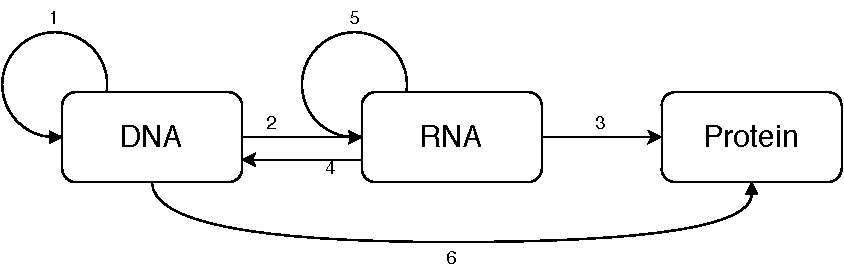
\includegraphics[width=1\linewidth]{figure/01-introduction/central-dogma} 

}

\caption{The central dogma of molecular biology. The dogma stipulates that sequence changes (that is the addition, removal or mutation of elements) can only occur in the direction of the arrows. 1. DNA replication 2. Transcription 3. Translation 4. Reverse transcription 5. RNA replication 6. Direct DNA-protein translation.}\label{fig:central-dogma}
\end{figure}
The importance of these molecular alterations to phenotypic change is exemplified in the developmental stages of human life. Humans start as a single cell and after roughly nine months are transformed into a multicellular organism with trillions of cells, including hundreds of unique cell types. As these cells arise from a single progenitor, they must contain identical genetic sequences (bar somatic mutations which occur at a low rate -- recently estimated to be roughly one mutation per cell division (14)). The process by which the body is able to create such diversely functioning cells and tissues, must come from regulation of how the genetic sequence is read and from the regulation of its products.

For reasons which I will describe in more detail later, DNA methylation is now being used widely by epidemiologists to try and understand how molecular changes, that do not involve direct sequence alterations, might result in variation amongst observable phenotypes. In order to understand how DNA methylation might influence observable phenotypes, one must first understand the role it plays within cells.

\hypertarget{dnam-as-part-of-regulation}{%
\section{DNA methylation as part of the regulatory machinery}\label{dnam-as-part-of-regulation}}

DNA methylation is correlated with gene expression levels and has been hypothesised to contribute to gene regulation (15--18). This is the main mechanism by which it is thought DNA methylation influences variability in phenotypes. However, DNA methylation is just one of many epigenetic marks that are involved in gene regulation (\textbf{Figure \ref{fig:epigenetic-marks}}). In this section I describe epigenetics and evidence gathered about the function of different epigenetic marks.


\begin{figure}

{\centering 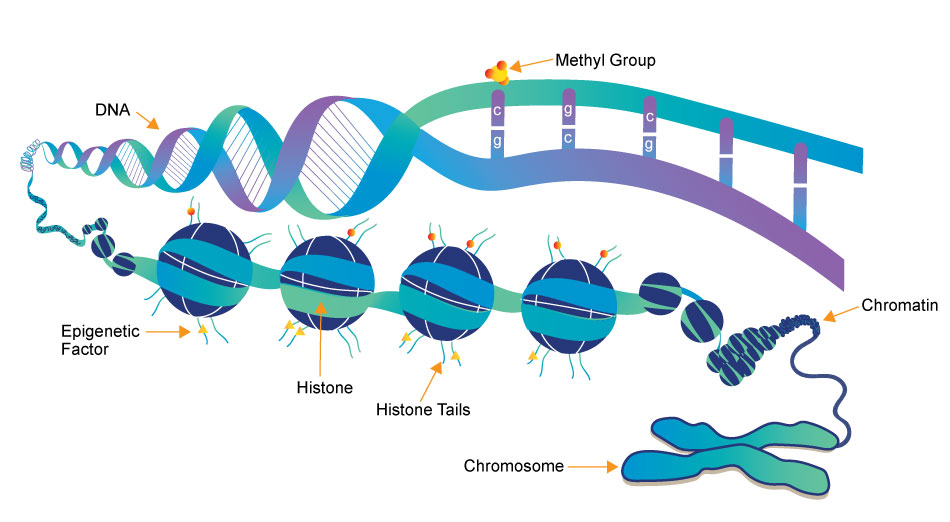
\includegraphics[width=1\linewidth]{figure/01-introduction/epigenetic-marks} 

}

\caption{Graphic of epigenetic marks taken from (19).}\label{fig:epigenetic-marks}
\end{figure}
\hypertarget{defining-epigenetics}{%
\subsection{Defining epigenetics}\label{defining-epigenetics}}

The definition of epigenetics is much debated (20). In the 1940s the `epigenetic landscape' was introduced by Waddington to describe how genes influence cell fates (21). Since then the term ``epigenetics'' has been used in many forms, so to avoid confusion, throughout the rest of the thesis, I will define epigenetics as: ``the study of mitotically (and potentially meiotically) heritable alterations in gene expression that are not caused by changes in DNA sequence'' (13). In an extension to this, epigenetic marks therefore refer to chemical changes to the genome and genome-bound proteins that are mitotically heritable (i.e.~changes that remain after cell division) and may influence gene expression without changing the DNA sequence.

\hypertarget{histone-modifications}{%
\subsection{Histone modifications}\label{histone-modifications}}

Histones are DNA-bound proteins that when modified can influence chromatin state and transcription factor interactions with the DNA (22). These proteins are contained in nucleosomes, which consist of four histone proteins, each of which is present twice in the nucleosome. Post-translational modifications can occur to any of the histone monomers and these have been associated with both positive and negative changes in gene expression (22--24). Histone modifications are numerous and complex in nature. To briefly describe the complexity, there are at least nine types of histone modification that can occur (25), each of the histone monomers can be modified across many different sites (23--25), and for any one site multiple of the same modification can occur (23,24). It is the combination of modifications across all histones that plays a role in gene expression regulation (23,24). Furthermore, histone modifications are subject to rapid change upon environmental stimulus to help induce or repress gene expression (22). The complexity of histone modifications, and the practical difficulties in collecting or assaying samples to assess these epigenetic marks, remains a barrier to their wide-spread measurement for use in population-based analyses (1). They may become far more prominent in the future as our understanding and ability to measure the modifications in a meaningful way increases.

\hypertarget{dna-methylation}{%
\subsection{DNA methylation}\label{dna-methylation}}

DNA methylation is the addition of a methyl group to DNA, which primarily occurs at the 5' cytosine of a CpG site. Little is known about the role of non-CpG site DNA methylation in humans and current EWAS tend to only measure CpG methylation. Two papers initially suggested that the function of this epigenetic mark was to repress gene expression (26,27). Since then, association with various important intracellular processes such as X-inactivation, genomic imprinting and suppression of transposon action have been elucidated (27--29). This genomic modification is also conserved amongst a wide variety of species, including various bacteria, plants, fungi, and mammals (18,30--32). Interestingly, one of the hypothesised functions of DNA methylation -- protection against `parasitic genomic sequences' -- is common to both human cells and bacterial cells (18,30). However, the relationship with gene expression may not be the same in prokaryotic organisms (30). Despite the abundance of research conducted in the area in the last 50 years, the role DNA methylation plays in regulating gene expression within human cells is not fully understood and research is still ongoing.

One thing research has revealed is that the location of DNA methylation is important to its relationship with gene expression. CpG sites are not randomly distributed throughout the genome but are often found in clusters (18) and it is thought that methylation and de-methylation of CpG sites in groups, is what drives their association with regulatory function (18). Clusters known as `CpG islands' are found at the majority of protein coding genes and constitute small areas of the genome that are enriched for CpG sites (18,33). The location of these islands as well as other CpG sites relative to genes and other regulatory elements is also of importance. Several studies have shown that higher levels of DNA methylation at transcription start sites tends to be associated with a lower levels of gene expression (18,34,35), but gene body DNA methylation is positively correlated with expression (\textbf{Figure \ref{fig:dnam-functions}}) (36,37). This suggests that regulation of DNA methylation in clusters at specific sites relative to genes is important in determining observed relationships with gene expression. Supporting this, there are clear biological processes that regulate DNA methylation at nearby sites together, for example, CpGs at transcription factor binding sites can be de-methylated as a group when the transcription factor binds (38). Further, nearby sites are often correlated (39,40). However, there is no evidence to suggest that neighbouring sites do indeed act in tandem or whether it is likely one site from the group is driving regulatory function. This is something I explore in \textbf{Chapter \ref{h2ewas-chapter}}.

These strong associations between DNA methylation and gene expression do not necessarily mean that the addition or removal of methyl groups will actively impact gene expression. Elucidating the causal nature of the association between DNA methylation and gene expression has been fraught with difficulties and has often provided conflicting results. One study showed an enzyme that catalyzes the addition of methyl groups to the DNA, DNA methyltransferase 3A, is required in haematopoeitic stem cells for them to differentiate, suggesting gene expression changes required for differentiation were not possible without addition of methyl groups to the DNA (41). However, studies have provided evidence that DNA methylation is unlikely to initiate the `silencing' of gene expression and may occur at transcription start sites of genes after they've already been repressed (42,43). To further complicate things, if DNA methylation does influence gene expression, the mechanism of action is unclear and may depend on the gene being examined. One study showed the presence of DNA methylation at the binding sites of the transcription factor, \emph{MYC}, was inversely associated with its binding (44), but another study suggested the presence of DNA methylation didn't have the same impact on the binding of the transcription factor, \emph{SP1} (45). Although the body of work presented in this thesis does not aim to explore if and how DNA methylation influences gene expression, it is important to note the relationship between the two isn't clear when thinking of the implications of DNA methylation-trait associations (46). This will be discussed further in the following sections.


\begin{figure}

{\centering 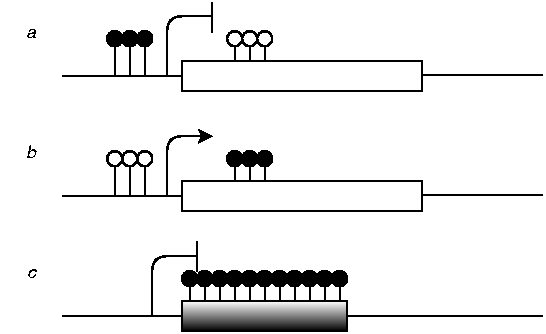
\includegraphics[width=1\linewidth]{figure/01-introduction/dnam-gene-expression} 

}

\caption{Simplified diagrams of the associations between DNA methylation and gene regulation. In \emph{a}, CpG sites are methylated at the promoter region, but not in the gene body, which is associated with lack of gene expression. In \emph{b}, the opposite is occurring.}\label{fig:dnam-functions}
\end{figure}
\hypertarget{dnam-phs}{%
\section{Population-based studies of DNA methylation associations}\label{dnam-phs}}

The importance of DNA methylation in disease has already been established in rare developmental disorders caused by aberrant imprinting patterns (47,48), but the relationship between DNA methylation and complex traits is unclear and is the focus of this thesis. In this section I discuss the study of complex traits, the appeal of studying DNA methylation for public health, introduce the most common study design to assess DNA methylation-trait associations, EWAS, and overview some successes and complications of the work.

\hypertarget{studying-complex-trait-associations}{%
\subsection{Studying complex trait associations}\label{studying-complex-trait-associations}}

Using DNA methylation in population-based studies, comprises studying its association with complex traits, which are phenotypes that are caused by a myriad of factors. The phenotypic value of any complex trait can be partitioned into its corresponding genetic (\(G\)) and environmental effects (\(E\)) like so
\begin{equation}
    z = G + E
    \label{eq:phenotypic-values}
\end{equation}
Both the environmental and genotypic values can further be partitioned into various effects (49). It's important to remember that DNA methylation itself is a complex trait and thus methylation of DNA at a given CpG site, is the result of a variety of genetic and environmental factors (18). However, unless explicitly stated, when discussing complex traits, I will be referring to human health and socio-economic outcomes rather than molecular phenotypes such as DNA methylation and gene expression.

Phenotypic values for any complex trait will vary across the population as each individual has a unique genomic sequence (except monozygotic twins) and is exposed to a variety of different environments, both external and internal.

Studying the associations between complex traits and other measures across the population can help deduce the aetiology of that trait, but phenotypic values may also covary with measures that have no implication for that traits aetiology. Identifying these covariations can still be useful for phenotype prediction.

It should be noted that different fields of study may have different views on the importance of certain measures. As discussed, there is evidence that DNA methylation may be inconsequential to gene expression changes (42,43), making it an unattractive measure to study when interested in the aetiology of cellular phenotypes in molecular biology. However, for epidemiological studies, understanding how DNA methylation covaries with complex traits could help provide useful predictors and further could yet yield insights into the underlying biology of complex traits. This will be explained in more detail in the coming sections.

\hypertarget{appeal-of-dnam}{%
\subsection{The potential value of DNA methylation measures to epidemiologists}\label{appeal-of-dnam}}

Epigenetic modifications are of potential interest to those studying any phenotype. Arguably, epigenetics could be required at some level for all phenotypic changes and, if causal, could be the difference between individuals who develop disease and those who do not (50). Further, epigenetic marks are modifiable, which means theoretically it would be possible to prevent or treat disease by altering such epigenetic patterns of individuals (51). There are large practical issues with this, which are discussed in more detail in \textbf{Section \ref{problems-for-ewas}}. However, even if targeting epigenetic marks is not easy, as long as it is possible to observe them, they could be used as diagnostic biomarkers and predictors (1,50,52,53). Thus, the ability to measure, and the research in to understanding epigenetic mechanisms, could have broad consequences for public health.

A major difference between DNA methylation and other epigenetic marks, is that DNA methylation is more stable. Enzymes do exist that can actively de-methylate the DNA, for example the ten-eleven translocation (TET) enzymes, but cell division or excision of the nucleotide is required for full de-methylation of a DNA molecule (54,55). Biologically, this suggests DNA methylation might be involved in long-term repression of gene expression, which is thought to be the case for X-inactivation (56), and practically it makes studying the epigenetic mark easier because stability ensures the marks are more resistant to changes after collection of samples. Also, even though it isn't clear that DNA methylation precedes gene expression regulation, the regulatory processes that govern whether genes are transcribed are linked. There are known examples of how DNA methylation tends to associate with other epigenetic marks, including positive correlation with the histone modification H3K9me3 (18) and histone deacetylation (18,57). This means measuring DNA methylation may capture regulatory information, even if addition or removal of methyl groups to the DNA would have little impact on gene expression. Recently, it has been shown that epigenetic marks can be used to predict each other with high accuracy (58), adding weight to the argument DNA methylation measurements capture far more than just DNA methylation itself.

\hypertarget{ewas}{%
\subsection{Epigenome-wide association studies}\label{ewas}}

When considering designing a study to assess whether one trait associates with another, one should have \emph{a priori} hypotheses or evidence that suggest studying the association would be of relevance to scientific understanding and public health. For studying the association between DNA methylation and complex traits, there is an abundance of evidence suggesting this could yield results of relevance. I've already explained why this may be: no phenotypic change is possible without some molecular change, DNA methylation is a relatively easy molecular measurement to make and it is known to highly correlate with an important component of cellular regulation -- gene expression. Further, DNA methylation has the potential to improve upon the prediction of complex traits beyond what can be done with current epidemiological and clinical measures.

EWAS are the most common study design for assessing the association between DNA methylation and a complex trait. They typically involve measuring hundreds of thousands of DNA methylation sites across the genome in a case-control or cohort setting and using linear models to assess the association between DNA methylation and the trait of interest.

Ideally, in every sample used in an EWAS, DNA methylation would be measured across all sites in the genome. Unfortunately, this is not currently possible and sequencing technologies that offer something similar are often very expensive. There are three alternatives available to DNA methylation studies. Firstly, one could sequence a small portion of the genome if this section is of particular interest, however this candidate gene approach is unlikely to be profitable unless the genes targeted already have good evidence for epigenetic variation with the trait of interest. As complex traits are polygenic (49) and we have incomplete knowledge of their underlying biology, a hypothesis-free approach, that samples from as much of the genome as possible, is preferable. Secondly, measuring DNA methylation on repeat sequences of the genome, such as long interspersed nuclear elements (LINEs) and short interspersed nuclear elements (SINEs), can provide estimates for global DNA methylation changes (59). These measurements indicate if a trait is related to large perturbations of DNA methylation across the genome, but give little mechanistic insight into what effects these changes may be having, as methylation at functional genes is not measured. Thirdly, one could employ an array approach that covers DNA methylation genome-wide at selected sites. This last approach is the most common for population-based studies as it enables measurement of DNA methylation at hundreds of thousands of sites at a relatively cheap price per sample (60). Without capabilities to measure methylation at every site in the genome, one must decide which sites are worth measuring. Current commonly used array technologies include the Illumina Infinium HumanMethylation450 (HM450) Beadchip and the Illumina Infinium HumanMethylationEPIC (HMEPIC) Beadchip, which measure DNA methylation at over 450,000 sites and over 800,000 sites respectively. They cover roughly 1.5-4\% of CpG sites in the genome (61). In order to capture what was thought to be the most relevant DNA methylation sites in relation to complex traits, the probes were chosen to map to 99\% of RefSeq genes (62). One reason for which this might have been done, is to help improve interpretation of EWAS findings. Identifying methylation changes at a specific gene suggests investigating the relationship of that gene and the complex trait further may yield interesting results, whereas interpreting complex trait associations with DNA methylation at a site in a relatively uncharacterized region of the genome would be more difficult for obvious reasons.

To measure DNA methylation, these array technologies, as well as sequencing techniques, often begin with bisulphite conversion of the DNA (63). This converts any un-methylated cytosine base to uracil and leaves methylated cytosines unchanged (64). The DNA samples can then be distributed amongst the array and the probes on the array will bind cytosines present at the regions their sequence corresponds to to (64). If a probe binds its target cytosine, then it will fluoresce, and this can fluorescence can be quantified to give `beta values'. Beta values range between zero and one, with zero corresponding to no methylation across all DNA samples at the target cytosine and one corresponding to methylation across all DNA samples at the target cytosine. DNA methylation is by nature a binary measurement, but mixtures of DNA samples (i.e.~multiple cells) mean that a continuous variable is generated unless single cell procedures are adopted.

This study design has been widely adopted over the past ten years and the relationship between a plethora of traits, from smoking to anthropometric measures to childhood adversities, and DNA methylation has now been studied (65--68). There are also large consortia that are pooling samples to gain power for these studies, for example the Pregnancy and Childhood Epigenetics (PACE) consortium (69). A few traits have been identified as being associated with large variations in DNA methylation, one of which is smoking, where strong associations across thousands of sites have been identified and many replicated in EWAS of smoking (65). It has been revealed that the association at some sites is driven by smoking causing changes in DNA methylation and over time these DNA methylation changes may be (mostly) reversible by giving up smoking (70). Also, DNA methylation can be used to predict smoking status, and one study has provided evidence that DNA methylation of a single locus can predict smoking status with high accuracy (71). Another measure shown to relate to large variation in DNA methylation across the genome is age. Similarly to smoking, DNA methylation makes a highly accurate predictor for age and is thought to be able to establish whether rate of `biological' aging is different from chronological aging (72--74). These studies have shown that large perturbations in the DNA methylome can be related to complex traits and highlight the potential for EWAS to identify accurate predictors for these traits.

\hypertarget{problems-for-ewas}{%
\subsection{Problems for EWAS}\label{problems-for-ewas}}

Despite the promise of understanding the underlying biological processes related to traits, studying the relationship between DNA methylation and complex traits provides many practical difficulties that often make the results of EWAS hard to interpret (1).

\hypertarget{confounding}{%
\subsubsection{Confounding}\label{confounding}}

One issue that plagues all observational epidemiology, including EWAS, is confounding. This is where the traits of interest share a common cause, which can generate effects and bias effect estimates, hindering correct interpretation of the association between traits. Complex traits are strongly correlated with each other, often in clusters, which can lead to large amounts of measured and unmeasured confounding being present in EWAS. Of course, in order to produce therapies to prevent or treat disease by altering DNA methylation or other parts of the epigenome, causality must be established. Therefore, problems of confounding must be overcome in EWAS to use these results to start developing methods of targeting DNA methylation changes, this is discussed more in \textbf{Section \ref{establishing-causality}}.

\hypertarget{cell-type-heterogeneity}{%
\subsubsection{Cell type heterogeneity}\label{cell-type-heterogeneity}}

As discussed, epigenetic factors guide differentiation of a single pluripotent cell to hundreds of cell types in human development. As these cell types can have large differences in morphology and function, it is clear that epigenetic marks, including DNA methylation, will vary between cell types (75,76). This poses two distinct problems for EWAS. Firstly, when collecting samples to measure DNA methylation, unless cells are purified, then a pool of cell types will be present in the samples, each with their own distinct DNA methylation patterns. This can lead to issues of confounding by cell type. For example, in a case control study, cases may be more likely to have increased numbers of CD4+ Th2 immune cells and these cells may on average have a higher level of DNA methylation at site X. In this scenario if one were to take blood cells, measure DNA methylation, and assess the association between DNA methylation and the trait of interest, one might find an association between DNA methylation at site X and the trait, but this may just be function of the increased number of CD4+ Th2 cells present in cases and site X may have no causal relationship with the trait itself. There have been efforts to try and account for cell type heterogeneity in EWAS (75,77,78), but to completely prevent its confounding effects, cells should be collected from a homogenous tissue or purified. In addition to, generating false positives, this confounding could mask true effects found within specific cell types. The second problem arising from cell-type specific patterns of DNA methylation is the uncertainty that the cell type being studied is one in which DNA methylation covaries with the trait of interest. Non-invasive cells to collect, such as blood, skin, and saliva, are common amongst epidemiological studies, but it is unclear whether EWAS in these studies are relevant to a large proportion of complex traits. This is studied, with regards to blood, in \textbf{Chapter \ref{h2ewas-chapter}}. Studies have actually shown high levels of correlation between DNA methylation across cell types at many CpGs (79), but it is unknown whether the correlated sites are important to trait variation. Further, this correlation may complicate interpretation of EWAS findings with regards to translational potential. Some organs, such as the brain, are difficult to target with therapies so even if a promising epigenetic target is identified, it may be almost impossible to translate this into something clinically useful.

\hypertarget{measuring-dna-methylation}{%
\subsubsection{Measuring DNA methylation}\label{measuring-dna-methylation}}

DNA methylation arrays face certain technical issues. Some probes map to SNPs, which can lead to incorrect detection of DNA methylation, others map to multiple sites across the genome (i.e.~are non-specific) and others may cross-hybridise. Batch effects can also substantially bias results in EWAS (2). Considerable effort has been made to characterise the arrays to identifiy potentially faulty probes (80,81) and methods developed (some originally for use in RNA-based studies) to help correct for batch effects (82--84). In \textbf{Chapter \ref{properties-of-ewas}} I explore the extent to which batch effects tend to be removed in current EWAS and whether EWAS results are enriched for potentially faulty probes not removed by study authors.

\hypertarget{complexity-of-regulatory-mechanisms}{%
\subsubsection{Complexity of regulatory mechanisms}\label{complexity-of-regulatory-mechanisms}}

EWAS identify single sites in the genome for which DNA methylation variation is associated with a trait of interest. As discussed, DNA methylation at a single site will likely be correlated with DNA methylation at neighbouring sites and other nearby epigenetic marks. This makes inferring mechanism of action very difficult. Differentially methylated region (DMR) analysis is often employed, which aims to determine if multiple neighbouring sites share an association with the trait of interest with the same direction of effect (40,76). These give evidence as to whether the sites covary similarly with the trait of interest, but do not provide evidence that the sites are acting independently or not. There are ways to circumvent the issues of biological complexity, but without additional gene expression data these often involve assuming the genes immediately adjacent to DNA methylation changes are of importance to the trait. However, no systematic evaluation of whether this assumption holds true for the majority of cases has been conducted.

\hypertarget{treatments}{%
\subsubsection{Treatments}\label{treatments}}

Currently there are therapies used in the clinic that target enzymes responsible for epigenetic alterations, for example DNA methyltransferase inhibitors and histone deacetylase inhibitors (85,86). They are primarily used to treat cancers, but as with many cancer treatments, are highly toxic. These therapies impact the epigenome globally and do not target any specific regions of the genome. This makes them highly undesirable for most diseases and as of yet there are no epigenetic therapies targeting specific regions of the genome. Methods, such as adapting CRISPR-cas9 enzymes, are being used in laboratories to alter DNA methylation at specific sites (87), and some have even achieved \emph{in vivo} targeted epigenetic modulation in mice (88). However, it is unclear whether these techniques can be scaled up for clinical use in humans and how long it may take to overcome the various complications.

In summary, there is great potential for EWAS to identify sites in the genome that could be targeted for treatment, but there are several challenges still to overcome. A great importance should be placed on using the data available to inform future designs of EWAS to maximise the potential of these studies.

\hypertarget{genetics-in-ewas}{%
\section{Using methods from genetics to help inform future EWAS}\label{genetics-in-ewas}}

In order to remedy some of the problems EWAS face and to help understand whether the ``experiment'' of measuring DNA methylation across many epidemiological cohorts and studies has been successful, we can borrow ideas and methods developed in genetics and genetic epidemiology.

Genetics is concerned with ascertaining the connection between traits and genetic variation. Germline genetic variants, the units of measurement for genome-wide association studies (GWAS), are fixed from conception and the association between these variants and complex traits tends to be unconfounded (89,90). Therefore, the properties of these variants and DNA methylation are different and one would expect the genetic and epigenetic architectures of complex traits to differ. However, genetic epidemiologists have had to overcome problems to help interpret GWAS, which are also pertinent to EWAS. These include understanding how much trait variation is captured by all the variants used in the study and how to infer function from genetic variation. Further, cataloging genetic associations has proven an invaluable resource for the research community (91) and these variants can be used as tools to augment the understanding of DNA methylation-trait associations. In this section I briefly describe some examples of these efforts and explain how they might be adapted to help inform future EWAS.

\hypertarget{gwas-catalog}{%
\subsection{Catalogues of genome-wide associations}\label{gwas-catalog}}

Cataloging genome-wide associations has a broad range of applications for researchers, from replication of GWAS, to identifying overlapping GWAS signals between traits, to pooling the data to try and understand the genetic architecture of complex traits as a whole. There are multiple databases now available to the genetic epidemiologist community that have catalogued these associations. These include manually curated databases of publicly available GWAS data, The GWAS Catalog, (91) and the IEU Open GWAS Project (92). A corollary database for EWAS is likely to also provide value for epigenetic epidemiologists. At the very least it would provide an easy tool to assess whether results replicate. Catalogues such as EWASdb (93) and the EWAS Atlas (94) are currently available but fall short of some key researcher requirements including ease of use and access to full summary statistics. The development of a new database, The EWAS Catalog, is the focus of \textbf{Chapter \ref{ewas-catalog}}.

\hypertarget{heritability}{%
\subsection{Total variance captured by all sites measured genome-wide}\label{heritability}}

In addition to cataloguing the information gained, efforts also need to be made in understanding the epigenetic architecture of complex traits to enable interpretation of these data.

As discussed, the phenotypic value of any trait can be partitioned into genetic effects and environmental effects. Thus, the variation of phenotypic values are the function of the genetic variance (\(\sigma^2_{G}\)) and environmental variance (\(\sigma^2_{E}\)),
\begin{equation}
    \sigma^2_{z} = \sigma^2_{G} + \sigma^2_{E}
    \label{eq:phenotypic-variance}
\end{equation}
The environmental effects could be split into an infinite number of different factors, most of which would negligibly influence the phenotypic variance. Knowing the extent to which each factor contributes to phenotypic variation is important for two reasons. Firstly, if a factor substantially influenced phenotypic variation then by modifying that factor one could modify the phenotypic values across a population. Secondly, one can identify which factors may best predict phenotypic values within a population. Currently, it is unknown how much variation in complex traits is attributable to DNA methylation changes. As discussed, assessing whether DNA methylation effects complex traits is difficult, but understanding whether they covary can still help quantify its total predictive capacity. Further, understanding how DNA methylation, as measured in contemporary EWAS, covaries with complex traits can help give insight on the validity of current study designs.

Many EWAS have been conducted and few have identified strong associations that capture substantial complex trait variation. Tissue types used and sites measured may partially explain this. It is a possibility that DNA methylation might not covary with many complex traits, or it could be that the associations between DNA methylation at individual sites are numerous, but the associations at each site are too small to detect with current sample sizes.

By combining information across all sites measured, one could quantify the total variation captured by DNA methylation for a complex trait of interest and so could properly assess the utility of association studies using the tissue types and sites measured.

Methods have already been developed to assess the total contribution of genetic variants measured in GWAS to complex trait variation (95,96) and in \textbf{Chapter \ref{h2ewas-chapter}}, I repurpose these methods developed to estimate the proportion of phenotypic variance correlated with DNA methylation across a range of phenotypes.

\hypertarget{inferring-biology-from-signals}{%
\subsection{Inferring biology from signals}\label{inferring-biology-from-signals}}

As discussed, the complexity of cellular processes makes it difficult to infer what consequences a change in methylation at a specific site may have. Similarly, for the majority of SNPs identified in GWAS, the functional change that relates to an association between genetic variation at that site and the trait of interest is unclear. Complex traits themselves are the result of a large number of complicated biological pathways that are determined by potentially thousands of gene products. It is often assumed that the signal from GWAS highlight genomic regions of importance to the trait and thus as a step to investigate the nature of the signal, sites identified are mapped to nearby genes. These genes can then be mapped to pathways and gene set enrichment analysis performed to assess whether the genes identified are present in any particular pathways more than expected by chance. This method has been adopted by epigenetic epidemiologists for use to examine EWAS signal (97). Given the DNA methylation probes on contemporary arrays were chosen specifically based on their proximity to protein coding genes, this gene mapping technique may actually be more valid for CpG sites.

Establishing causality from DNA methylation signal is difficult (See \textbf{Sections \ref{dnam-phs} \ref{establishing-causality}}). Thus, when applying gene set enrichment analyses to identify prominent pathways in EWAS signals, the pathways identified may be downstream consequences of one or many confounders rather than of aetiological relevance to the trait of interest. Further, the EWAS signals, and therefore pathways they might influence, may be a consequence of trait variation. This is important to remember when interpreting the results of such an analysis, but it doesn't render the results useless. There is a huge body of work that characterises gene action and relationships of this gene action with various traits. By mapping EWAS signals to genes and pathways, a path between the trait (or a confounder) and changes in DNA methylation might become clearer. One example of this comes with EWAS of smoking, that have consistently identified DNA methylation at the \emph{AHRR} gene (65,98--101). This gene is known to play a role in handling toxic substances found in tobacco smoke (102,103). Thus, large changes in DNA methylation related to this gene points towards epigenetic changes at that locus influencing the cellular response to smoking. This shows, that despite difficulties in interpreting EWAS findings and subsequent pathway analysis, EWAS can actually add to the pool of information about underlying trait biology when used in conjuncture with other evidence.

Understanding both the causes and consequences of complex traits are pertinent to intervening on health outcomes. As EWAS has the potential to identify both, it could identify important facets of trait biology missed by GWAS studies; however, it is unclear as to whether the analogous gene set enrichment design adopted by EWAS is currently adding to the information discovered by GWAS. In \textbf{Chapter \ref{ewas-gwas-comp-chapter}} I compare overlap of GWAS and EWAS signals in this context and discuss the use of both study designs in elucidating underlying trait biology.

\hypertarget{establishing-causality}{%
\subsection{Establishing causality}\label{establishing-causality}}

\hypertarget{mendelian-randomization}{%
\subsubsection{Mendelian randomization}\label{mendelian-randomization}}

As discussed, population-based studies of DNA methylation suffer from the same limitations as any observational epidemiology study, namely confounding and reverse causation. One method that aims to mitigate confounding is Mendelian randomization (MR) (89,90,104), which uses genetic variants as proxies for the exposure of interest in an instrumental variable framework (illustrated in \textbf{Figure \ref{fig:mr-diagram}}). Using genetic variants as instruments has the advantage that the direction of effect will always be from instrument to exposure and not vice versa, making interpretation of the studies simpler. Furthermore, unlike environmental phenotypes, that tend to be highly correlated and clustered into groups, genetic variants associated with a trait tend to be unconfounded (89,90). In the absence of assortative mating, genetic variants should be distributed randomly across the population, so in effect those grouped by genotype should exhibit differences in exposure, but confounding factors should not differ between genotype groups (90). Assortative mating has been reliably shown to occur with some traits such as social behaviours and anthropometric measures (105--107). Assortment tends to occur on visible social factors and so intentional assortment based on DNA methylation profiles is very unlikely. However, DNA methylation may associate with factors that are assorted on, for example alcohol consumption (108,109), which may lead to unintentional assortment on DNA methylation profiles. The impact this may have on MR studies using DNA methylation has not been explored, and this analysis is beyond the scope of this thesis but is something that should be noted when assessing the reliability of such MR studies.

\hypertarget{availability-of-data-for-mr}{%
\subsubsection{Availability of data for MR}\label{availability-of-data-for-mr}}

Another advantage of MR is the data it uses. Thousands of GWAS have been conducted giving researchers ample instruments for a wide variety of traits and many of these instruments are easily accessible through databases such as the GWAS Catalog (91) and IEU Open GWAS Project (92). Furthermore, it isn't necessary to use individual-level data to conduct MR studies; summary statistics from GWAS are all that is needed to provide data in a two-sample MR framework (110,111). This is especially valuable to conducting MR studies using DNA methylation data as DNA methylation is not widely measured across cohorts and case-control studies. Thus, without a method to combine summary data from both GWAS of DNA methylation and GWAS of other complex traits, well-powered MR studies would not be possible to assess the potential effect of DNA methylation on complex traits (and \emph{vice versa}).

\hypertarget{assumptions-of-mr}{%
\subsubsection{Assumptions of MR}\label{assumptions-of-mr}}

In order for MR analyses to be valid, they must satisfy three instrumental variable assumptions, these are illustrated in \textbf{Figure \ref{fig:mr-diagram}}. Testing assumption one, the instruments associate with the exposure of interest, is simple, but the other two assumptions cannot technically be proven to be true. Horizontal pleiotropy, where genetic variants associate with more variables than just the exposure of interest, can lead to violations in assumptions two and three. Ideally, MR would be performed in the context where the genetic effect on the exposure had been characterised such that the mechanism of action was understood clearly. This would help give evidence against assumptions two and three being broken. Unfortunately, this is rarely possible. However, a plethora of methods have now been developed to test for pleiotropic effects, given the exposure of interest has multiple independent genetic variants reliably associated with it.


\begin{figure}

{\centering 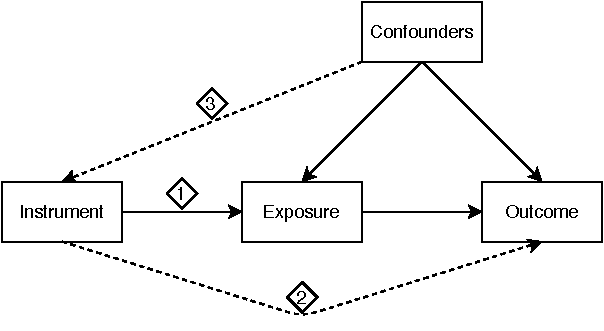
\includegraphics[width=1\linewidth]{figure/01-introduction/mr-diagram} 

}

\caption{Mendelian randomization. Mendelian randomization can be used to test the causal nature of exposure-outcome relationships provided the assumptions are met. Assumption 1. There is an association between the instrument and the exposure. Assumption 2. There are no associations between the instrument and outcome, except through the exposure. Assumption 3. The instrument is not associated with any factors that confound the exposure-outcome relationship.}\label{fig:mr-diagram}
\end{figure}
\hypertarget{applying-mr-in-a-dna-methylation-context}{%
\subsubsection{Applying MR in a DNA methylation context}\label{applying-mr-in-a-dna-methylation-context}}

MR can be applied to studies of DNA methylation by using methylation quantitative trait loci (mQTL), genetic variants associated with changes in DNA methylation levels, as proxies for DNA methylation variation (50,112,113). As mentioned previously, using a two-sample MR framework is especially useful to help increase power for these studies (50). For each DNA methylation site few independent mQTLs have been identified (3), which prevents the use of various tests to examine whether the instruments are likely to be pleiotropic. Further, without reliable associations between SNPs and DNA methylation at some sights, MR cannot be conducted. Both cis-mQTLs (mQTLs within 1Mb of the DNA methylation site) and trans-mQTLs (mQTLs over 1Mb away from the DNA methylation site) have been identified in GWAS of DNA methylation variation. As genetic architecture of DNA methylation changes is also not well understood, the mechanism of action for each mQTL can only be speculated at present. Cis-mQTLs are thought to be less likely to be pleiotropic than trans-mQTLs as the mechanism of action seems more likely to be related to the binding of regulatory machinery that may influence DNA methylation levels (112,114). For example, a genetic variant may decrease the affinity of a transcription factor for that region and so the transcription factor will bind less frequently and/or for a shorter period, this would lead to increased methylation at that site (115). On the contrary, the mechanism of trans-mQTL action, especially those on separate chromosomes to the DNA methylation site of interest, is more likely to be pleiotropic (114), for example a trans-mQTL could influence gene expression of a transcription factor that binds many sites and alters their DNA methylation (116), this would make the trans-mQTL associate with multiple DNA methylation sites. Therefore, if one limits mQTLs to those in cis, this gives greater confidence that horizontal pleiotropy isn't biasing results.

Due to the complexity of cellular regulatory mechanisms (\textbf{Section \ref{dnam-as-part-of-regulation}}), it may be impossible to identify the exact cause of changes in complex traits, even with replicated MR results that give strong evidence of an effect of DNA methylation on a complex trait.

As mentioned, DNA methylation varies both temporally and across cell types. If the instruments used to represent DNA methylation are viewed as influencing life-time differences in DNA methylation between individuals, then temporal variation can be ignored. However, cell type-specific effects are likely to occur for some mQTLs. One could imagine a scenario in which blood cells require a specific gene (gene A) to be expressed that is completely useless in adipose cells, which could mean all adipose cells have 100\% DNA methylation at the promoter region of gene A. Thus, any genetic variants that associate with DNA methylation variation in blood would not also associate with variation in adipose cells.

With all this in mind, it is important to maintain the idea that making strong conclusions of causality in the context of DNA methylation is difficult, but triangulating evidence from multiple sources could be key to understanding the role of DNA methylation in underlying trait biology (117).

Such evidence can come from different sources of statistical methodology that can be used to assess causality in observational studies (118--120). One that has been applied in EWAS includes taking advantage of temporal measurements (121). If DNA methylation is measured before the trait of interest, then chances of reverse causation are greatly diminished, although confounding may still be an issue. DNA methylation associations may also be tested across different, relevant tissue types and molecular biology can be used to augment epidemiological evidence. Tools exist to experimentally manipulate DNA methylation at specific regions of the genome in cultured cells or in model organisms (87,88). Using a negative control design, one could follow up any findings from an epidemiological study like an EWAS, in the laboratory by assessing if changes in the DNA methylation sites identified have any intracellular impact. This could be done for a variety of tissue types of interest.

To truly provide strong evidence that changes in DNA methylation is causally related to a trait, one must take a cross-disciplinary approach.

\hypertarget{overview-of-thesis-aims}{%
\section{Overview of thesis aims}\label{overview-of-thesis-aims}}

DNA methylation has great potential for use in an epidemiological sense and as samples with DNA methylation data continue to grow it is important to understand the limitations of EWAS and how to maximise it's potential. My thesis aims to address this by exploring what information has been gained from EWAS (\textbf{Chapters \ref{ewas-catalog} and \ref{properties-of-ewas}}), what information is still to gain from EWAS (\textbf{Chapter \ref{h2ewas-chapter}}), whether EWAS might add to our biological understanding of complex traits above GWAS (\textbf{Chapter \ref{ewas-gwas-comp-chapter}}) and by applying MR in a particular case, the potential for confounding in EWAS (\textbf{Chapter \ref{dnam-lung-cancer-mr}}). See the flowchart in \textbf{Figure \ref{fig:thesis-flowchart}} for a graphical depiction.

In \textbf{Chapter \ref{ewas-catalog}} a database of published EWAS is curated and made publicly available, which will be used in later chapters. The aim of \textbf{Chapter \ref{properties-of-ewas}} is to analyse the results present in this database jointly to allow the discovery of commonalities across methylome-trait associations and provide a platform to explore what is driving these commonalities. Further, the chapter explores the extent to which published results are reliable by assessing replication rate and whether sites measured by unreliable probes are prominent.

After exploring the information already gained from EWAS, \textbf{Chapter \ref{h2ewas-chapter}} investigates the information still to gain from EWAS. The aim of the chapter is to apply methods developed to assess SNP-heritability to estimate the proportion of complex trait variation that is associated with sites commonly measured in EWAS.

\textbf{Chapter \ref{ewas-gwas-comp-chapter}} will then aim to assess whether the discoveries of EWAS may provide extra biological insight for traits of interest on top of those from GWAS. Tests will be applied to assess whether there is more overlap between the sites, genes or pathways identified by some large EWAS (N \textgreater{} 4500) and their corresponding GWAS than expected by chance.

Finally, \textbf{Chapter \ref{dnam-lung-cancer-mr}} will apply MR to explore the causal nature of associations between DNA methylation and lung cancer. This application case-study will compare and contrast findings to conventional EWAS estimates to give an example of the potential residual confounding that can be present in EWAS.


\begin{figure}

{\centering 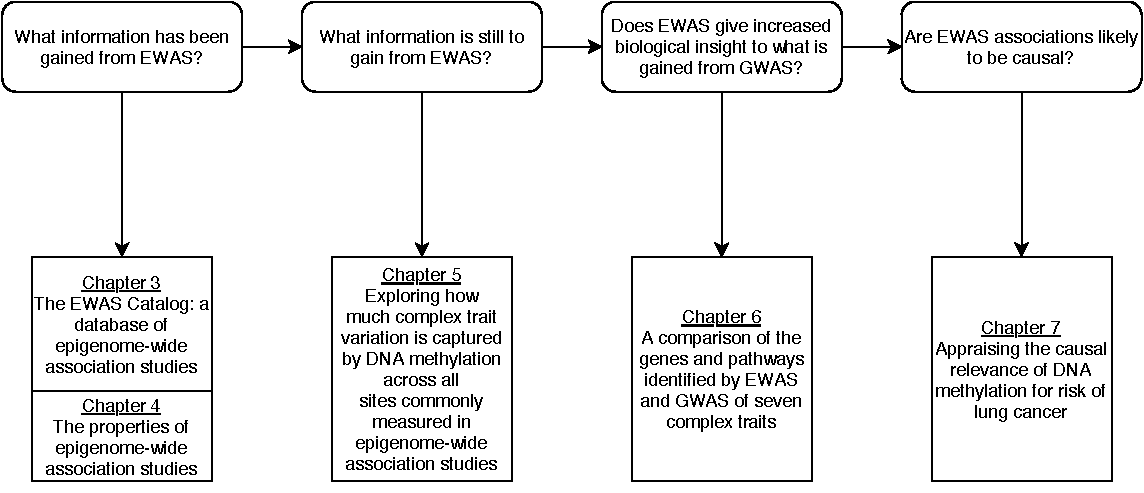
\includegraphics[width=1\linewidth]{figure/01-introduction/thesis-flowchart} 

}

\caption{Flowchart showing questions being asked in the thesis and the corresponding chapters attempting to help answer them.}\label{fig:thesis-flowchart}
\end{figure}
\hypertarget{methods}{%
\chapter{Methods}\label{methods}}

\hypertarget{ewas-catalog}{%
\chapter{The EWAS Catalog: a database of epigenome-wide association studies}\label{ewas-catalog}}

\hypertarget{abstract-03}{%
\section{Abstract}\label{abstract-03}}

In recent years, the increase in availability of DNA methylation measures in population-based cohorts and case-control studies has resulted in a dramatic increase in the number of EWAS being performed and published. To make this rich source of molecular data more accessible, a manually curated database has been made containing CpG-trait associations (at P \textless{} 1x10\textsuperscript{-4}) from published EWAS, each assaying over 100,000 CpGs in at least 100 individuals. The database currently contains these associations from 178 published EWAS as well as full summary statistics for over 180 million association tests of 427 EWAS in the Avon Longitudinal Study of Parents and Children (ALSPAC) and the Gene Expression Omnibus (GEO). It is accompanied by a web-based tool and R package that allow these associations to be easily queried. This database provides a platform for analyses in Chapter 4 and 6. Further, it will give other researchers the opportunity to quickly and easily query EWAS associations to gain insight into the molecular underpinnings of disease as well as the impact of traits and exposures on the DNA methylome. The EWAS Catalog is available at: \url{http://www.ewascatalog.org}.

\hypertarget{introduction-03}{%
\section{Introduction}\label{introduction-03}}

Epigenome-wide association studies (EWAS) aim to assess the associations between phenotypes of interest and DNA methylation across the genome (50,63,122). These associations may then be used for disease diagnosis or prediction (50,63,122). Also, unlike genetic variants, changes in DNA methylation are responsive to the environment and so may be targeted for treatment. EWAS of smoking (65), body mass index (BMI) (67) and aging (72) have shown that various exposures are related to large perturbations in DNA methylation across the genome. Furthermore, a paper recently estimated that over 60\% of the total proportion of BMI variation was captured by DNA methylation at about 150 CpG sites (123). In recent years, there has been a dramatic increase in the number of EWAS being performed and published due to technological advancements making it possible to measure DNA methylation at hundreds of thousands of CpG sites cheaply and effectively. Giving researchers easy access to EWAS outputs will help them gain insight into the molecular underpinnings of disease as well as the impact of traits and exposures on the DNA methylome. Furthermore, current collections of summary statistics have already proven useful to various fields, for example the GWAS Catalog (91) has been cited over 2000 times in papers contributing to new methods and exploring the genetic architecture of a plethora of traits.

At the time of making the database, to our knowledge, there were no databases that had collected well-curated EWAS on all traits (not just diseases) in an online database accessible to researchers. During production one database fulfilled those metrics: EWAS Atlas (94). Other databases are available but are limited to certain diseases (e.g.~MethHC (124)). The EWAS Atlas provides a simple-to-use website with annotated CpG sites and information on traits. Ideally a database of EWAS results will provide summary statistics, including betas, standard errors and p-values where provided from publications, in an easily accessible manner, this enables researchers to explore various aspects of the published data without having to retrieve the published article. For example, researchers might compare effect estimates between studies in the database or check to see if their results are replicated in another published study. At the time of writing, the EWAS atlas platform did not enable users to download effect estimates and standard errors. Another caveat is that there is currently only published data on the platform, not full summary statistics from EWAS.

The EWAS Catalog aims to improve upon current databases to 1) allow easy and programmatic access to summary statistics for downstream analyses by researchers and 2) provide full summary statistics from a range of EWAS conducted in multiple cohorts. To this end we have produced The EWAS Catalog, a manually curated database of currently published EWAS, 387 EWAS performed in the Avon Longitudinal Study of Parents and Children (ALSPAC) (125,126) and 40 EWAS performed from data from the Gene Expression Omnibus (GEO) database. The process and data inclusion are summarised in \textbf{Figure \ref{fig:catalog-project-workflow}}.


\begin{figure}

{\centering 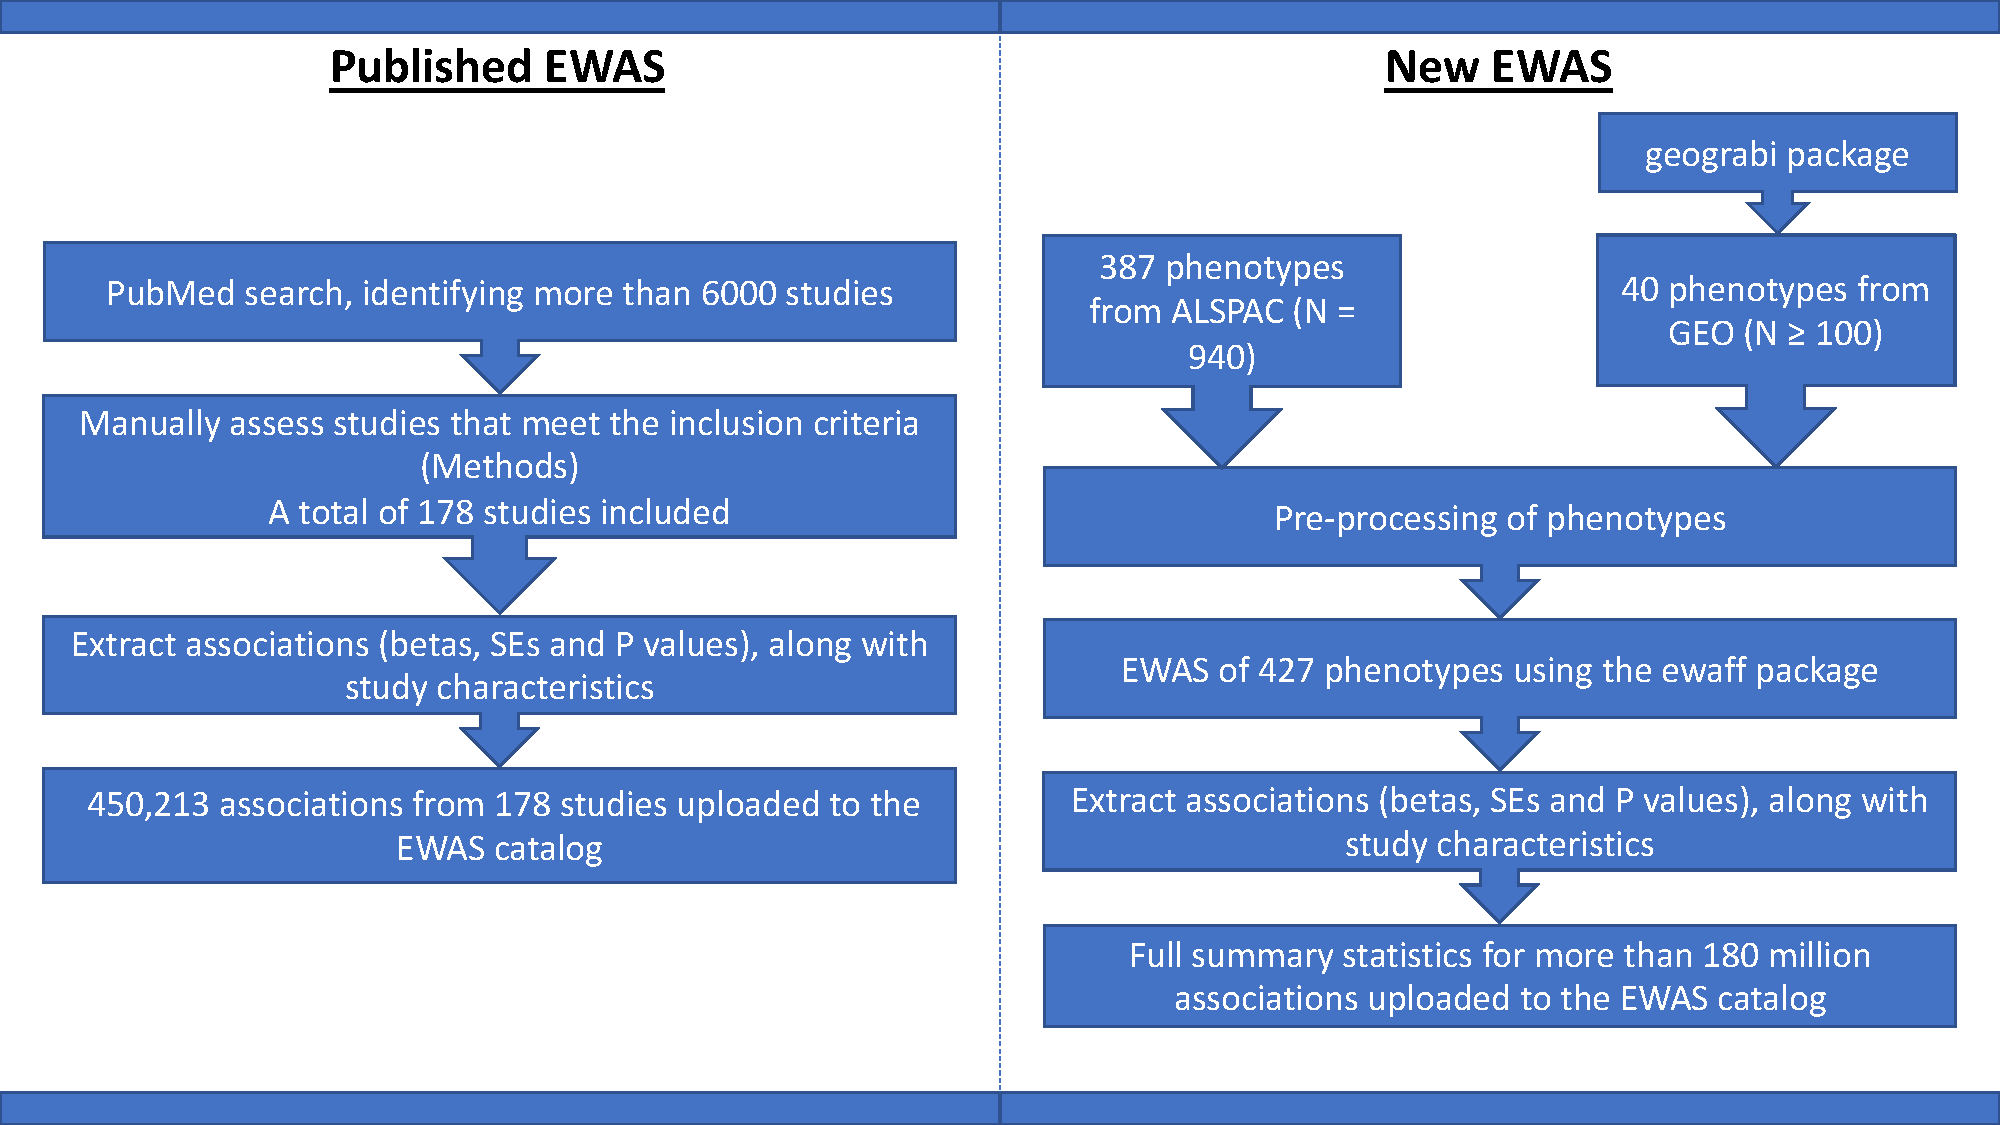
\includegraphics[width=1\linewidth]{figure/03-ewas_catalog/project_flowchart} 

}

\caption{\textbf{Project flowchart.} On the left is a brief description of how the CpG-phenotype associations were assembled from published works and on the right is a brief description of the EWAS performed using individual level data.}\label{fig:catalog-project-workflow}
\end{figure}
I am not responsible for all the work presented in this chapter. Dr James Staley built the original website. Dr Matthew Suderman has been key in development, and maintenance of the website. Dr Paul Yousefi extracted data from GEO. All three also provided (and continue to provide) expert knowledge to adapt the database to optimise user experience. There was also a team to help gather and input the data. I helped develop and maintain the website, gather and input the data, ran all the EWAS using data from the ALSPAC cohort and the GEO database. The team, led by myself, is continuing to develop and maintain the database. Full acknowledgements to the team can be found on the website: \url{http://www.ewascatalog.org/about/}.

\hypertarget{methods-03}{%
\section{Methods}\label{methods-03}}

\hypertarget{implementation}{%
\subsection{Implementation}\label{implementation}}

The EWAS Catalog web app was built using the Django Python package (\url{https://djangoproject.com}). The data is stored in a combination of MySQL databases and fast random access files (64) and can be queried via the web app or the R package (www.github.com/ewascatalog/ewascatalog-r/).

\hypertarget{overview-of-publication-data-extraction}{%
\subsection{Overview of publication data extraction}\label{overview-of-publication-data-extraction}}

To identify publications, periodic literature searches are performed in PubMed using the search terms: ``epigenome-wide'' OR ``epigenome wide'' OR ``EWAS'' OR ``genome-wide AND methylation'' OR ``genome wide AND methylation''.

Our criteria for inclusion of a study into The EWAS Catalog are as follows:
\begin{enumerate}
\def\labelenumi{\arabic{enumi}.}
\tightlist
\item
  The EWAS performed must contain over 100 humans
\item
  The analysis must contain over 100,000 CpG sites
\item
  The DNA methylation data must be genome-wide
\item
  The study must include previously unpublished EWAS summary statistics
\end{enumerate}
CpG-phenotype associations are extracted from studies at P \textless{} 1x10\textsuperscript{-4}. All these criteria along with the variables extracted are documented on the website (www.ewascatalog.org/documentation). Experimental factor ontology (EFO) terms were mapped to traits to unify representation of these traits. These EFO terms were manually entered after looking up the trait in the European Bioinformatics Institute database (www.ebi.ac.uk/efo).

Based on these criteria, from 2020-09-08, The EWAS Catalog contained 450213 associations from 605 studies.

\hypertarget{overview-of-geo-data-extraction}{%
\subsection{Overview of GEO data extraction}\label{overview-of-geo-data-extraction}}

To recruit additional datasets suitable for new EWAS analysis, the geograbi R package (\url{https://github.com/yousefi138/geograbi}) was used to both query GEO for experiments matching The EWAS Catalog inclusion criteria (described above) and extract relevant DNA methylation and phenotype information. The query was performed by Dr Paul Yousefi on 20 March 2019 and identified 148 such experiments with 32,845 samples where DNA methylation and phenotype information could be successfully extracted. From these, the aim was to repeat the analyses performed in the publications linked by PubMed IDs to each GEO record. Thus, I looked up the corresponding full texts for each dataset and identified the main variables of interest. Of the 148 putative GEO studies, only 34 (23\%) contained sufficient information to replicate the original analysis.

\hypertarget{ewas-methods-03}{%
\subsection{EWAS methods}\label{ewas-methods-03}}

\hypertarget{alspac-03}{%
\subsubsection{Avon Longitudinal Study of Parents and Children (ALSPAC)}\label{alspac-03}}

EWAS were conducted for 387 continuous and binary traits in peripheral blood DNA methylation of ALSPAC mothers in middle age (N = 940), generated as part of the Accessible Resource for Integrated Epigenomics Studies (ARIES) project (127).

ALSPAC recruited pregnant women in the Bristol and Avon area, United Kingdom, with an expected delivery date between April 1991 and December 1992 (\url{http://www.bris.ac.uk/alspac/}). Over 14,000 pregnancies have been followed up (both children and parents) throughout the life-course. Full details of the cohort have been published previously (125,126). The EWAS performed for the EWAS catalog were done so using phenotypic and DNA methylation data from the mothers (N = 940).
All continuous and binary phenotypes were extracted from the same timepoint that blood was drawn for DNA methylation assays.

Ethical approval for ALSPAC was obtained from the ALSPAC Ethics and Law Committee and from the UK National Health Service Local Research Ethics Committees. Written informed consent was obtained from both the parent/guardian and, after the age of 16, children provided written assent. The study website contains details of all the data that is available through a fully searchable data dictionary (\url{http://www.bristol.ac.uk/alspac/researchers/access/}).

Study data were collected and managed using REDCap electronic data capture tools hosted at ALSPAC (128,129). REDCap (Research Electronic Data Capture) is a secure, web-based software platform designed to support data capture for research studies, providing 1) an intuitive interface for validated data capture; 2) audit trails for tracking data manipulation and export procedures; 3) automated export procedures for seamless data downloads to common statistical packages; and 4) procedures for data integration and interoperability with external sources.

Ancestry principal components were generated within ALSPAC mothers using PLINK (v1.9). Before analysis, genetic data went through quality control and were imputed as follows.

Mothers were genotyped using the Illumina human660W-quad genome-wide single nucleotide polymorphism (SNP) genotyping platform (Illumina Inc., San Diego, CA, USA) at the Centre National de Génotypage (CNG; Paris, France). SNPs were removed if they displayed more than 5\% missingness or a Hardy-Weinberg equilibrium P value of less than 1.0e-06. Additionally, SNPs with a minor allele frequency of less than 1\% were removed. Samples were excluded if they displayed more than 5\% missingness, had indeterminate X chromosome heterozygosity or extreme autosomal heterozygosity. Samples showing evidence of population stratification were identified by multidimensional scaling of genome-wide identity by state pairwise distances using the four HapMap populations as a reference, and then excluded. Cryptic relatedness was assessed using a IBD estimate of more than 0.125 which is expected to correspond to roughly 12.5\% alleles shared IBD or a relatedness at the first cousin level. Related subjects that passed all other quality control thresholds were retained during subsequent phasing and imputation.

Imputation of mother's genotype data in ALSPAC was done with ALSPAC children's data. So, genotypes in common between the sample of mothers and sample of children were combined. SNPs with genotype missingness above 1\% due to poor quality were removed along with subjects due to potential ID mismatches. We estimated haplotypes using ShapeIT (v2.r644) which utilises relatedness during phasing. We obtained a phased version of the 1000 genomes reference panel (Phase 1, Version 3) from the Impute2 reference data repository (phased using ShapeIt v2.r644, haplotype release date Dec 2013). Imputation of the target data was performed using Impute V2.2.2 against the reference panel (all polymorphic SNPs excluding singletons), using all 2186 reference haplotypes (including non-Europeans).

After quality control and imputation, independent SNPs (r2 \textless{} 0.01) were used to calculate the top 10 ancestry principal components.

For all traits, linear regression models were fitted with DNA methylation at each site as the outcome and the phenotype as the exposure. DNA methylation was coded as beta values between 0 and 1. For a particular site, a beta value of 0 represents no methylation being detected in all cells measured and a value of 1 represents all cells being methylated at that site. Covariates included age, the top 10 ancestry principal components, and 20 surrogate variables.

\hypertarget{transforming-phenotypic-data}{%
\subsubsection{Transforming phenotypic data}\label{transforming-phenotypic-data}}

Values of continuous phenotypes were defined as outliers and set to missing, then all phenotypes with 100 or more non-missing values were kept for further analysis. To ensure all phenotypes were approximately normal, each of their distributions were examined and then transformed. If a variable was deemed right-skewed, it was log-transformed then its distribution was re-assessed by eye. Square-roots and cube-roots were used to try and approximate normality if log-transformation did not work. If a variable was deemed left-skewed, it was squared, and the distribution re-assessed by eye.

\hypertarget{ewas-statistical-models}{%
\subsubsection{EWAS statistical models}\label{ewas-statistical-models}}

For all traits, linear regression models were fitted with DNA methylation as the outcome and the phenotype as the exposure as for the ARIES data. Twenty surrogate variables were included as covariates. Other covariates were considered, but surrogate variables only were used for two reasons: 1) to help automate the process and 2) because covariates used in the original EWAS were not included with many of the GEO datasets.

Statistical analyses were conducted in R (Version 3.3.3). The smartsva package (130) was used to create surrogate variables and the ewaff R package (\url{https://github.com/perishky/ewaff}) was used to conduct the EWAS, all p-values are two-sided.

\hypertarget{results-03}{%
\section{Results}\label{results-03}}

\hypertarget{database-interface-and-use}{%
\subsection{Database interface and use}\label{database-interface-and-use}}

There are two ways to access this large, curated database: through the main website www.ewascatalog.org or by using the R package ``ewascatalog''. The website provides a simple user interface, which resembles that of the GWAS catalog (91), whereby there is a single search bar to explore the database and links to tabs that contain documentation on the contents and how to cite its use (Figure 1). Users may enter a CpG, gene, genome position or trait into the search bar and it will rapidly return detail for relevant EWAS associations, including CpG, trait, sample size, publication and association (effect and P value) (Figure 1). This information along with additional information such as ancestry, outcome, exposure units, and tissue analysed are available for download as a tab-separated value (tsv) text file. Unlike other EWAS databases, we provide the option of downloading summary results for both the user's search and for the entire database.
\begin{figure}

{\centering 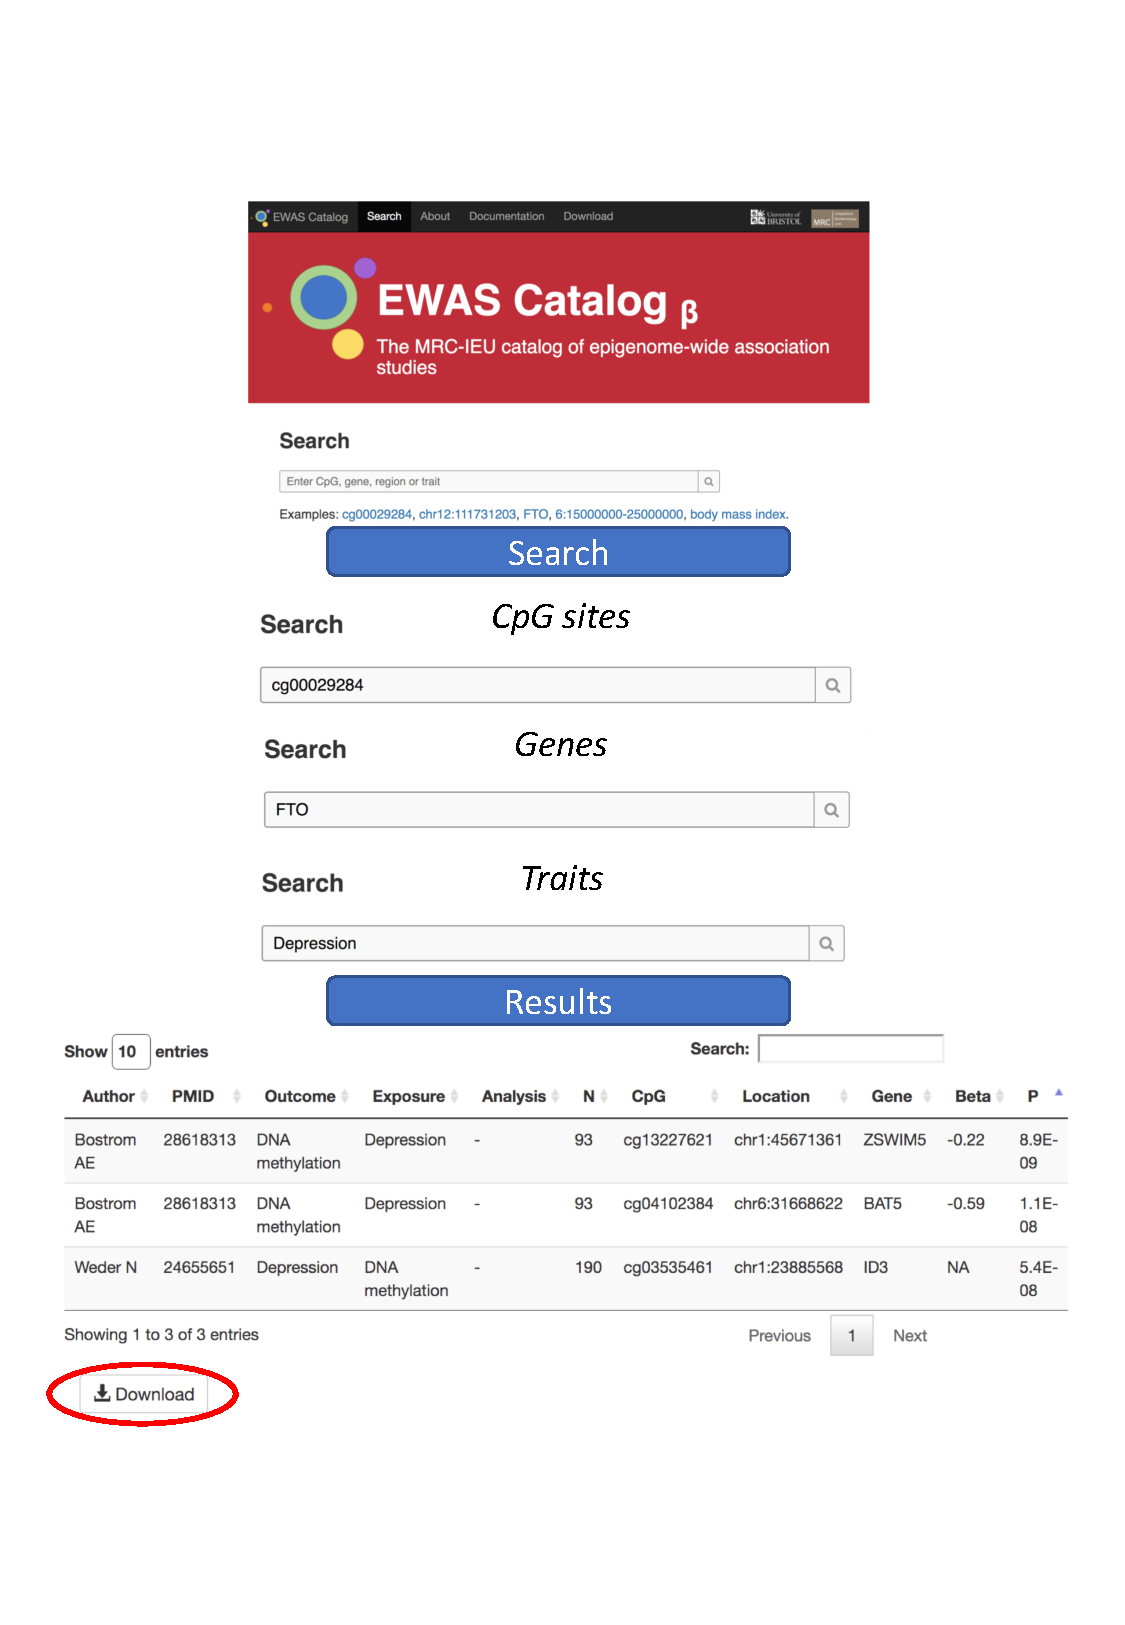
\includegraphics[width=1\linewidth]{figure/03-ewas_catalog/using_the_catalog} 

}

\caption{Using the EWAS catalog. 
At the top of the figures is the home page URL, ewascatalog.org. 
Below that are examples of three types of searches possible: 
1. CpG sites, 2. genes and 3. traits. 
Finally, the results are displayed after searching the catalog for “Depression”. 
Circled in red is the download button, this button enables the user to download the results of their search as a tab-separated value file. 
This file will contain the information shown on the website as well as additional analysis information.}\label{fig:catalog-use}
\end{figure}
The R package, along with installation instructions and examples are available at \url{https://github.com/ewascatalog/ewascatalog-r/}. Once installed, the database can be queried directly in R using the ``ewascatalog()'' function similar to the website: simply supply the function with a CpG site, gene, genome position or trait and the function returns the same output as is downloadable from the website.

\hypertarget{discussion-03}{%
\section{Discussion}\label{discussion-03}}

In this chapter, a database of previously published EWAS and the full summary statistics of 427 newly performed EWAS within ALSPAC and GEO has been established. This is freely available for all researchers to use and provides a platform to explore what information has been gained from EWAS as well as a platform that can be used to pool all existing data to gain new insights into both the EWAS study itself and how DNA methylation associates with traits. Despite the fact The EWAS Atlas has similar aims to The EWAS Catalog, the latter provides full summary statistics, extra information and a user-friendly platform to enable more downstream analyses.

The EWAS catalog team will continue to collate and upload newly published EWAS and further increase the number of full summary statistics on the website by performing additional EWAS on available datasets and by inviting EWAS authors to provide full summary statistics. Currently work is ongoing to include additional functionality to allow users to easily and systematically compare their EWAS findings to EWAS in the database. With this full summary data, it is possible to make greater strides into discovering the epigenetic architecture of traits.

Therefore, despite the fact no extra information about EWAS was presented in this chapter, a platform has been made that enables us to explore 1) what information has been gained from EWAS and 2) what could explain EWAS associations. This will be explored in the next chapter.

\hypertarget{properties-of-ewas}{%
\chapter{Properties of epigenome-wide association studies}\label{properties-of-ewas}}

\hypertarget{abstract-04}{%
\section{Abstract}\label{abstract-04}}

Understanding the nature of EWAS associations is imperative for biological inference from these studies. This understanding may also impact future study design. Of the data in the EWAS Catalog, 9.9\% of reported associations are from CpGs measured by unreliable probes and 20.8737864\% of studies did not account for both batch effects and cellular composition. Suggesting, some associations may be false positives. However, characteristics of DNA methylation also likely partly explain some EWAS associations - heritability and variability of DNA methylation explained 0.084\% of the variance of effect EWAS effect sizes. This study also identifies associations at sites common to multiple traits. cg06500161 \emph{ABCG1} associated with 71 traits, which were all traits relating to weight, metabolites or type-2-diabetes. This highlights the potential to use the data collected for the EWAS Catalog in \textbf{Chapter \ref{ewas-catalog}} to generate new hypotheses and connect DNA methylation changes to the broad range of potential phenotypic changes.

\hypertarget{introduction-04}{%
\section{Introduction}\label{introduction-04}}

Learning from successes and mistakes helps drive forward development. Hundreds of epigenome-wide association studies (EWAS) have been conducted in the last 10-15 years, yet no cross-EWAS studies, comparing results across a large group of EWAS results has been performed. By exploring the patterns of association across a large group of EWAS, one can discover potential explanations for the results found, that may shed light on failings in the literature as well as shared epigenetic architectures across traits.

Since the inception of EWAS, it has become clear that batch effects and cellular heterogeneity can generate false positives and bias effect sizes (2,76,79). However, there are examples of replication amongst EWAS results, (100,131--136) and further, use of triangulation can be used to bolster evidence that changes in DNA methylation estimated are unlikely due to bias. By way of an example, changes in DNA methylation at \emph{AHRR} have been replicated across multiple smoking EWAS (65,100,101,137) and as functional reaseach has implicated this gene in handling toxic substances found in tobacco smoke (138), it seems unlikely these findings are chance occurances.

The characteristics of the DNA methylome may also explain some EWAS findings. Heritability varies across DNA methylation sites (139,140), and so if genetic effects are driving associations, either through confounding or with DNA methylation as a mediator, one would expect heritable sites to be commonly identified in EWAS. Variance is also heterogenous across sites (141). Technical effects are more likely to influence DNA methylation variation at sites for which measured variation is low. Thus, some studies have advocated removing these sites to prevent reporting generating false positives and to reduce the multiple testing burden (142,143). However, it is unclear how variance in DNA methylation relates to the magnitude of effect estimates. Experimental studies have shown DNA methylation changes at different locations of the genome correlate with different regulatory functions. For example, an increase in DNA methylation at transcriptional start sites is correlated with a decrease in gene expression (18,34,35), but an increase in DNA methylation within a gene body shows the opposite association (36,37). Thus, genomic location of DNA methylation sites is likely to influence their likelihood of association with a trait.

Understanding underlying reasons that drive EWAS results is essential for future study design. This may come in the form of proper consideration of potential biasing factors, or by selecting certain DNA methylation sites based on their specific characteristics. Further, understanding the characteristics of DNA methylation-trait associations can inform the design of future technologies aimed at measuring DNA methylation for EWAS.

Also, by examining the commonalities of EWAS results, one has the potential to uncover links between traits that have not previously been made or to identify new potential mediating factors between traits.

In this study we first describe the data present in the EWAS Catalog before exploring various explanations for the findings.

\newpage

\hypertarget{methods-04}{%
\section{Methods}\label{methods-04}}

\hypertarget{epigenome-wide-association-studies-data}{%
\subsection{Epigenome-wide association studies data}\label{epigenome-wide-association-studies-data}}

All the data for the analysis were extracted from The EWAS Catalog (\textbf{Chapter \ref{ewas-catalog}}). This includes 178 published studies, 387 EWAS from the ARIES subsection of ALSPAC (\textbf{Section \ref{alspac-03}}) (125--127) and 40 EWAS performed using data from the gene expression omnibus (GEO) resource. See \textbf{Chapter \ref{ewas-catalog}} for more details.

\hypertarget{description-of-data}{%
\subsection*{Description of catalog data}\label{description-of-data}}
\addcontentsline{toc}{subsection}{Description of catalog data}

Associations between DNA methylation and traits, unless otherwise stated, were extracted at P \textless{} 1x10\textsuperscript{-7}. Each of the CpGs in the Catalog are annotated to genes, using data from the meffil R package .

T-statistics (\(t\)) were calculated using P-values, sample sizes (\(n\)) and the qt() function in R. \(r^2\) values were calculated from t-statistics as follows
\begin{equation}
    r^2 = \frac{t^2} {t^2 + n - 1}
    \label{eq:r-squared}
\end{equation}
We identified traits for which r\textsuperscript{2} values might be inflated. For each EWAS the estimated r\textsuperscript{2} values were summed and these values were transformed to approximate a normal distribution. Then a z-test was performed to assess which sum of r\textsuperscript{2} values were greater than the mean sum of r\textsuperscript{2} values. From the z-test, those with a FDR-corrected P-value of less than 0.05 were labelled as having inflated r\textsuperscript{2} values.

\hypertarget{identifying-faulty-probes}{%
\subsection{Identifying faulty probes}\label{identifying-faulty-probes}}

By far the most common method to measure DNA methylation across the studies in The EWAS Catalog is using the Illumina Infinium HumanMethylation450 Beadchip. Since its development, the array has been extensively characterised (2,76,79,80) and it was found that not all probes map just to the CpG they were designed to bind to. Some probes map to SNPs, others are non-specific and some are prone to cross-hybridisation. We assigned probes to be `potentially faulty' if they were characterised as such by Zhou et al.~(80).

\hypertarget{replication}{%
\subsection{Replication}\label{replication}}

An association was deemed to be replicated at P \textless{} 1x10\textsuperscript{-4}. We assessed replicability of EWAS within the database in two separate ways. Firstly, replication within studies is recorded in the EWAS Catalog, thus we simply performed a lookup for any studies that performed a replication or meta-analysed discovery and replication datasets. Secondly, we performed a lookup of results for any traits for which multiple EWAS had been conducted.

The Catalog also contains results from studies that have uploaded their data to GEO as well as results from the re-analysis of that data performed by The EWAS Catalog team. These re-analyses adjusted for 20 surrogate variables only as many studies did not provide a complete set of covariates to GEO. We performed a lookup of results found in the original EWAS in the re-analysed data.

\hypertarget{selecting-data-to-assess-dna-methylation-characteristics}{%
\subsection{Selecting data to assess DNA methylation characteristics}\label{selecting-data-to-assess-dna-methylation-characteristics}}

We decided to only use studies and results thought to be more ``robust'' when assessing how characteristics of DNA methylation might impact EWAS results. To this end, we removed all potentially faulty probes and probes that mapped to sex chromomsomes, excluded studies with likely inflated r\textsuperscript{2} values, and removed studies for which re-analysis of the data replicated less than 10\% of the findings.

\hypertarget{dna-methylation-characteristics}{%
\subsection{DNA methylation characteristics}\label{dna-methylation-characteristics}}

The association between heritability, variability and average level of DNA methylation at each CpG site and EWAS effect size was assessed. To allow this across traits, we standardised beta coefficients, \(\beta_{standard}\), like so,
\begin{equation}
    \beta_{standard} = \frac{\beta\sigma(x)} {\sigma(y)}
    \label{eq:standardised-beta-coeffs}
\end{equation}
As individual data were not available to us, the variance in DNA methylation sites was approximated by the variance in DNA methylation at sites as supplied by the Genetics of DNA Methylation Consortium (GoDMC) (144) and the trait variance was estimated by rearranging the equation \eqref{eq:r-squared-from-beta} depending on whether DNA methylation was the independent (\(x\)) or dependent (\(y\)) variable in the model.
\begin{equation}
    r^2 = \frac{\beta^2\sigma^2(x)} {\sigma^2(y)}
    \label{eq:r-squared-from-beta}
\end{equation}
GoDMC (144) also provided the mean levels of DNA methylation at each site. Heritability of DNA methylation at each site has been previously estimated by McRae et al.~2014 (139) and Van Dongen et al.~2016 (145), these values were kindly made publically available by the authors of those studies and were used in this study.

Associations between each characteristic and effect size were assessed using linear regression, fitting the standardised effect size as the dependent variable and the characteristic as the independent variable. The standardised effect sizes were rank normalised to ensure normality and remove the impact of outliers.

\hypertarget{enrichment-tests}{%
\subsection{Enrichment tests}\label{enrichment-tests}}

It was assessed whether the sites identified by EWAS that were present in the catalog were enriched in any genomic region etc. This analysis was performed using LOLA\ldots{}

\hypertarget{code-availability-04}{%
\subsection{Code availability}\label{code-availability-04}}

Code used to run the analyses is available here: \url{https://github.com/thomasbattram/something}

All analyses were completed using R (version 3.6.2).

\newpage

\hypertarget{results-04}{%
\section{Results}\label{results-04}}

\hypertarget{catalog-description}{%
\subsection*{Description of the catalog}\label{catalog-description}}
\addcontentsline{toc}{subsection}{Description of the catalog}

Before assessing what might be underlying various EWAS results, we present a brief summary of the data in the EWAS Catalog (\textbf{Table \ref{tab:study-data-tab}}). \linebreak
\begin{table}[!h]

\caption{\label{tab:study-data-tab}Description of data present in the EWAS Catalog}
\centering
\resizebox{\linewidth}{!}{
\begin{tabular}[t]{ll}
\toprule
study-trait & value\\
\midrule
\rowcolor{gray!6}  Number of EWAS & 614\\
Number of traits & 556\\
\rowcolor{gray!6}  Number of samples & 389527\\
Median sample size (range) & 536 (93 - 13474)\\
\rowcolor{gray!6}  Number of associations & 155976\\
\addlinespace
Number of CpGs identified & 129670\\
\rowcolor{gray!6}  Number of genes identified & 19305\\
Sex (\%) & Both (38.6), Females (52.0), Males (2.1)\\
\rowcolor{gray!6}  Ethnicities & EUR (75.3), Unclear (12.5), AFR (4.6), Other (3.6), ADM (1.6), EAS (1.4), SAS (1.0)\\
Age (\%) & Adults (72.5), Geriatrics (11.2), Children (4.9), Infants (4.4)\\
\addlinespace
\rowcolor{gray!6}  Number of tissue types & 42\\
Most common tissues (\%) & whole blood (84.14), cord blood (4.34), cd4+ t-cells (2.60), placenta (1.24), saliva (0.99)\\
\bottomrule
\end{tabular}}
\end{table}
\linebreak

It may be that certain regulatory mechanisms are more important to phenotypic differences between individuals. By analysing datasets such as the EWAS Catalog, it might be possible to identify which regions may be more important and further, it could be used to identify novel mediating factors between traits.

The number of traits each CpG associated with was fairly even across chromosomes (\textbf{Figure \ref{fig:traits-manhattan}}). There were five CpGs that associated with more than ten traits, cg01940273 \emph{-}, cg05575921 \emph{AHRR}, cg00574958 \emph{CPT1A}, cg17901584 \emph{DHCR24}, cg06500161 \emph{ABCG1}. cg06500161 \emph{ABCG1} associated with more traits than any other site - 71 traits. These correspond mostly to metabolites, weight-related traits, and type two diabetes.


\begin{figure}

{\centering 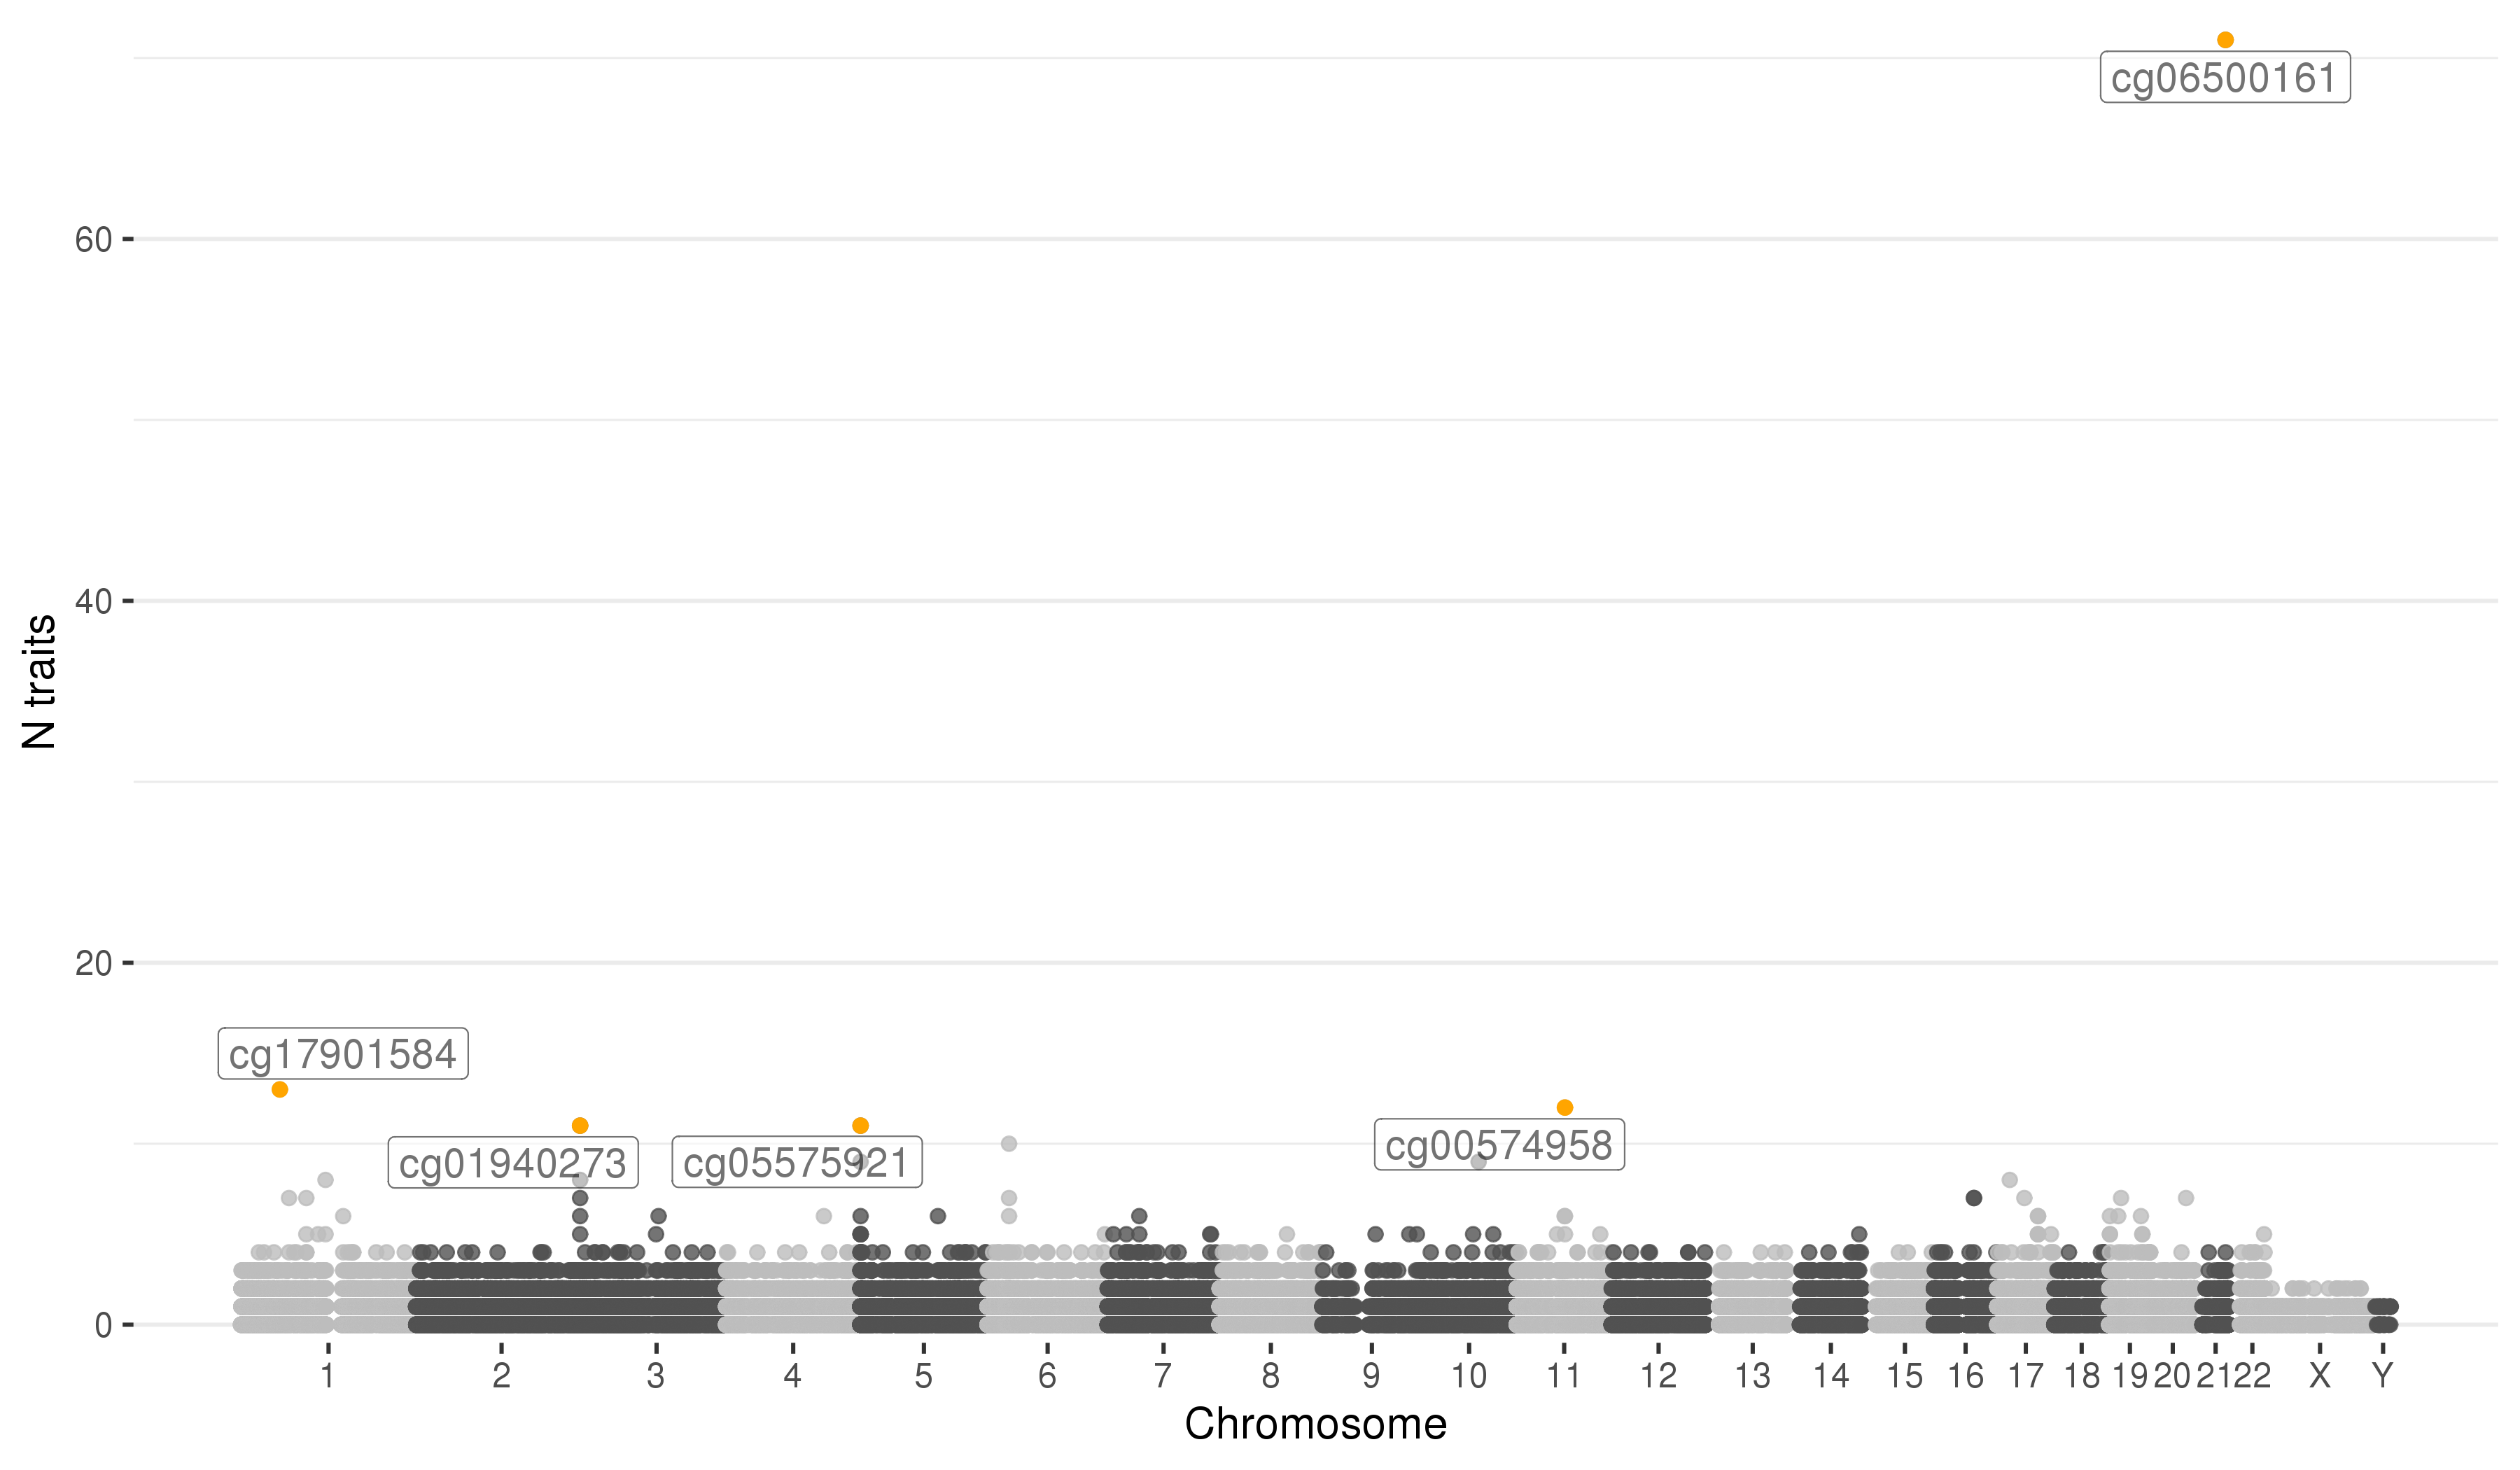
\includegraphics[width=1\linewidth]{figure/04-properties_of_ewas/traits_per_dmp_at_1e-07} 

}

\caption{\textbf{Number of unique traits associated with each DNA methylation at each CpG.} Sites associated with more than 10 unique traits are highlighted in orange and labelled.}\label{fig:traits-manhattan}
\end{figure}
Next we estimated the variance (see equation \eqref{eq:r-squared}) captured by each association to gauge the level of covariation between complex traits and DNA methylation.

The total trait variance correlated with DNA methylation (r\textsuperscript{2}) at each site varied from 0.0011 to 0.97 with a median of 0.093 (\textbf{Figure \ref{fig:rsq-distribution}}). The sum of r\textsuperscript{2} values ranged greatly from 0.0055 to 23,879 (\textbf{Figure \ref{fig:rsq-sum-distribution}}), with a median of 1.2. There was evidence that eight studies had a total sum of r\textsuperscript{2} values greater than the mean (FDR \textless{} 0.05) and r\textsuperscript{2} values from individual associations from these studies made up the majority of r\textsuperscript{2} values greater than 0.1 (\textbf{Figure \ref{fig:rsq-distribution}}). When excluding those studies from the results, the median r\textsuperscript{2} value at individual sites was 0.025.


\begin{figure}

{\centering 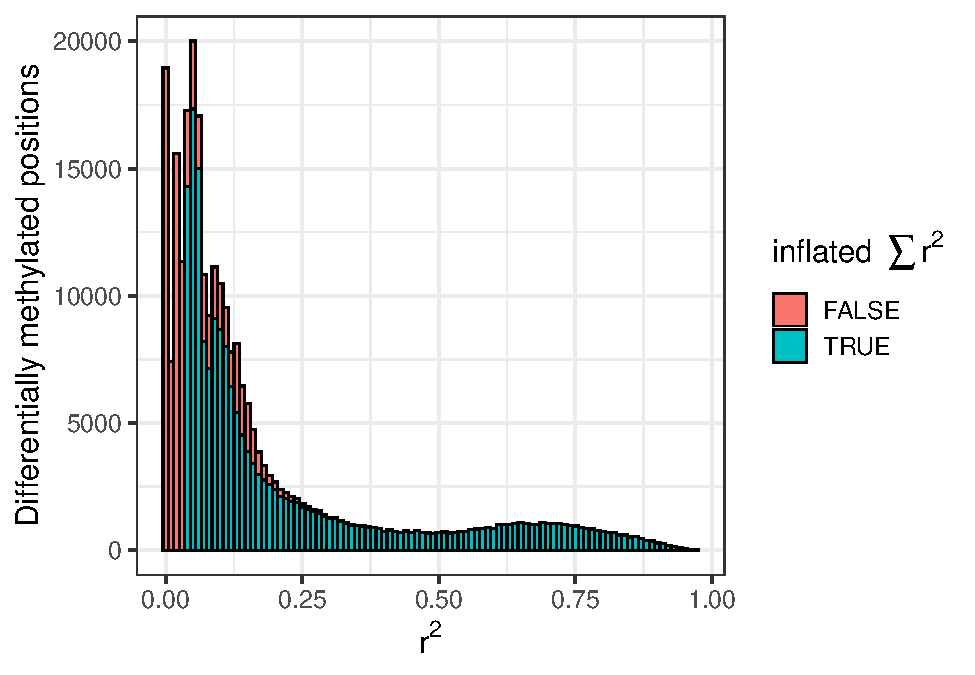
\includegraphics[width=1\linewidth]{thesis_files/figure-latex/rsq-distribution-1} 

}

\caption{\textbf{Distribution of r-squared values across all CpG sites in The EWAS Catalog}. Each EWAS can identify multiple differentially methylated positions, each of which will capture some variance of the trait of interest for that EWAS (r\textsuperscript{2}). \(\sum {r^2}\) is the sum of r\textsuperscript{2} values, the distribution of which is shown in \textbf{Figure \ref{fig:rsq-sum-distribution}}. Eight studies were identified for which there was strong evidence that the sum of r\textsuperscript{2} values were greater than the mean across all studies. All of the differentially methylated positions identified by those studies are highlighted in blue on the plot.}\label{fig:rsq-distribution}
\end{figure}

\begin{figure}

{\centering 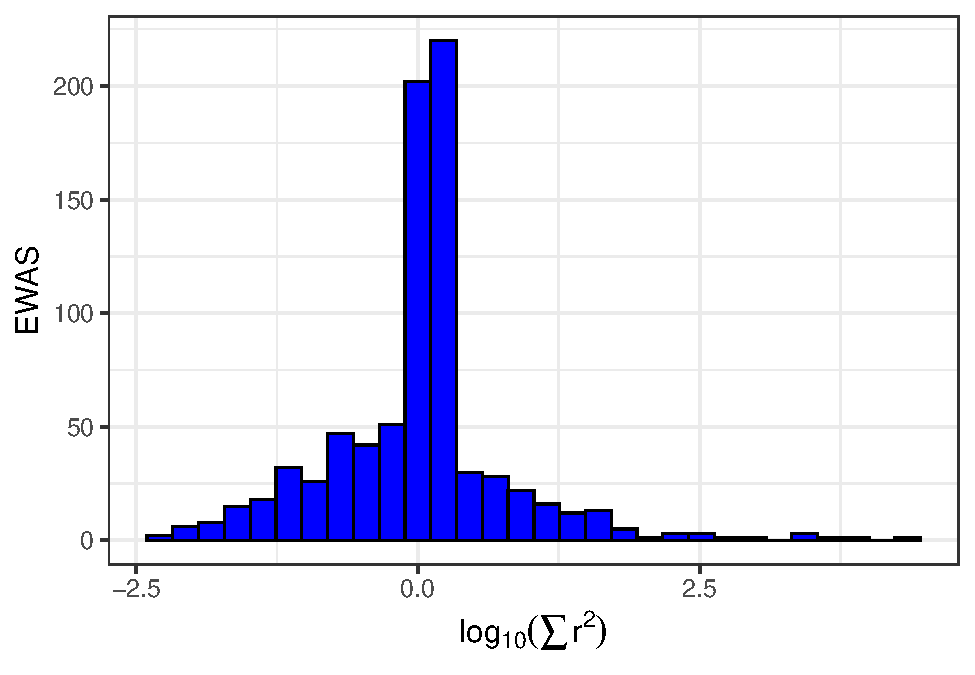
\includegraphics[width=1\linewidth]{thesis_files/figure-latex/rsq-sum-distribution-1} 

}

\caption{\textbf{Distribution of the sum of r\textsuperscript{2} values across each study in The EWAS Catalog.}}\label{fig:rsq-sum-distribution}
\end{figure}
These results suggest that some associations within the database are likely to be inflated, yet for most traits, variation at individual DNA methylation sites captures little trait variance. Summing the r\textsuperscript{2} values indicates a substantial proportion of trait variance can be captured by multiple DNA methylation sites for some traits, but this can only be estimated by jointly modelling the contribution of all sites to trait variance. This is explored in \textbf{Chapter \ref{h2ewas-chapter}}. Here, the sum of r\textsuperscript{2} values is used to indicate whether the results of a study are likely inflated and thus unlikely to be robust.

\hypertarget{robustness-of-results}{%
\subsection{Robustness of results}\label{robustness-of-results}}

Here we continue to explore the robustness of results to 1. identify potential improvements that could be made for future studies and 2. identify potentially erroneous associations to exclude from downstream analyses.

In at least one model, 579 studies adjusted for batch effects, 518 studies adjusted for cell composition, and 489 adjusted for both. Of all DMPs identifed, 9.3\% were measured by potentially faulty probes and an extra 0.64\% were present on sex chromosomes (\textbf{Figure \ref{fig:faulty-probes-plot}}).


\begin{figure}

{\centering 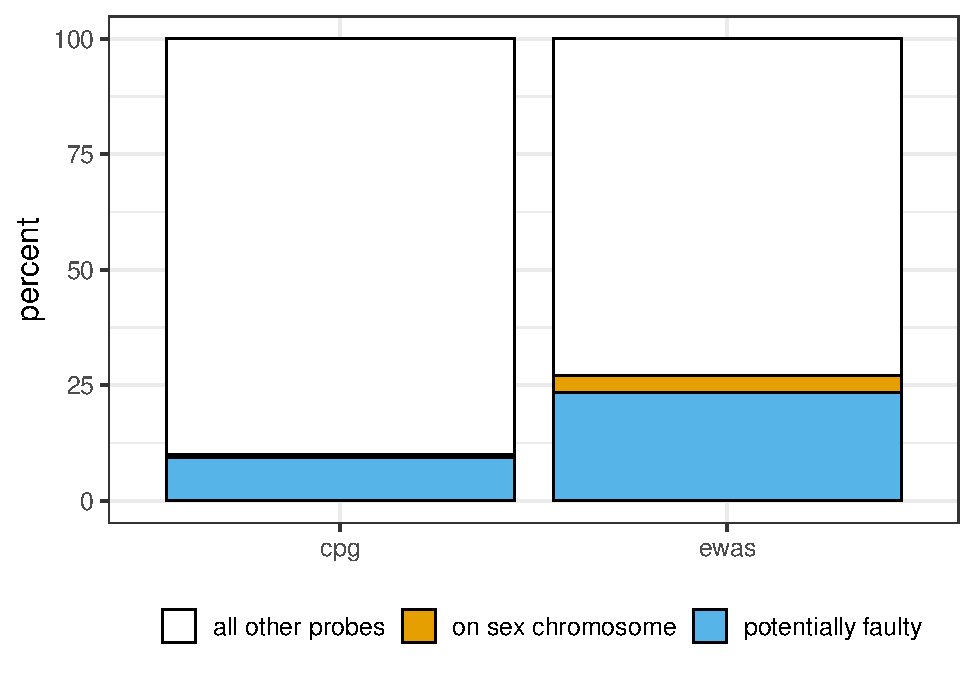
\includegraphics[width=1\linewidth]{thesis_files/figure-latex/faulty-probes-plot-1} 

}

\caption{\textbf{The percentage of differentially methylated positions that may have been identified by faulty probes and the percentage of EWAS that reported identifying at least one of these probes.} Some CpGs are both on a sex chromosome and were identified as faulty by Zhou et al.~They were labelled as `potentially faulty'.}\label{fig:faulty-probes-plot}
\end{figure}
There were 30 studies that performed a meta-analysis of discovery and replication samples. A further 48 studies performed a separate replication analysis. Together, this provides 1666 associations within the EWAS Catalog that have been replicated at P \textless{} 1x10\textsuperscript{-4}.

From the studies that put their data on GEO, we re-analysed the association between DNA methylation and the phenotype of interest from the original study, including 20 surrogate variables as covariates. Both the original study results and the results from the re-analysis of the phenotype of interest are in The EWAS Catalog database for 10 studies. Across the studies, between 0\% and 96.875\% of DMPs were replicated at P \textless{} 1x10\textsuperscript{-4} (\textbf{Table \ref{tab:geo-reanalysis-tab}}). \linebreak
\begin{table}[!h]

\caption{\label{tab:geo-reanalysis-tab}GEO re-analysis replication}
\centering
\resizebox{\linewidth}{!}{
\begin{tabular}[t]{llll}
\toprule
Trait & N-DMPs & N-replicated & Percent-replicated\\
\midrule
\rowcolor{gray!6}  Age at menarche & 1 & 0 & 0.00\\
Arsenic exposure & 11 & 0 & 0.00\\
\rowcolor{gray!6}  Arsenic exposure & 1 & 0 & 0.00\\
Fetal alcohol spectrum disorder & 19 & 1 & 5.26\\
\rowcolor{gray!6}  Inflammatory bowel disease & 14 & 13 & 92.86\\
\addlinespace
Nevus count & 1 & 0 & 0.00\\
\rowcolor{gray!6}  Psoriasis & 16 & 0 & 0.00\\
Rheumatoid arthritis & 47,875 & 116 & 0.24\\
\rowcolor{gray!6}  Smoking & 30 & 12 & 40.00\\
Smoking & 32 & 31 & 96.88\\
\bottomrule
\end{tabular}}
\end{table}
\linebreak

Using the Catalog data we further performed replication analyses. There were 62 studies that shared a common phenotype of interest. Replication rate, judged as the percentage of CpGs also present in any other study of the same trait with P value \textless{} 1x10\textsuperscript{-4}, varied from 0 to 100 between studies (\textbf{Table \ref{tab:replication-tab}}). \linebreak
\begin{table}

\caption{\label{tab:replication-tab}Replication rate}
\centering
\resizebox{\linewidth}{!}{
\begin{tabular}[t]{lllll}
\toprule
trait & n-cpgs & rep-cpgs & n-rep-studies & prop-rep\\
\midrule
\rowcolor{gray!6}  Smoking & 23 & 6 & 19 & 0.26087\\
Smoking & 15 & 1 & 19 & 0.06667\\
\rowcolor{gray!6}  Smoking & 17 & 14 & 19 & 0.82353\\
Rheumatoid arthritis & 51,476 & 8 & 1 & 0.00016\\
\rowcolor{gray!6}  Smoking & 972 & 766 & 19 & 0.78807\\
\addlinespace
Smoking & 25 & 5 & 19 & 0.20000\\
\rowcolor{gray!6}  Smoking & 29 & 25 & 19 & 0.86207\\
Smoking & 30 & 9 & 19 & 0.30000\\
\rowcolor{gray!6}  Birth weight & 15 & 0 & 4 & 0.00000\\
Body mass index & 3 & 3 & 8 & 1.00000\\
\addlinespace
\rowcolor{gray!6}  Depression & 4 & 0 & 2 & 0.00000\\
Smoking & 1 & 1 & 19 & 1.00000\\
\rowcolor{gray!6}  Maternal smoking during pregnancy & 185 & 7 & 1 & 0.03784\\
Schizophrenia & 1 & 0 & 2 & 0.00000\\
\rowcolor{gray!6}  Alzheimers disease Braak stage & 2 & 2 & 1 & 1.00000\\
\addlinespace
Alzheimers disease Braak stage & 100 & 2 & 1 & 0.02000\\
\rowcolor{gray!6}  Smoking & 37 & 35 & 19 & 0.94595\\
Maternal smoking in pregnancy & 25 & 10 & 2 & 0.40000\\
\rowcolor{gray!6}  Smoking & 53 & 48 & 19 & 0.90566\\
Birth weight & 1 & 0 & 4 & \vphantom{1} 0.00000\\
\addlinespace
\rowcolor{gray!6}  Maternal smoking in pregnancy & 22 & 19 & 2 & 0.86364\\
Smoking & 461 & 415 & 19 & 0.90022\\
\rowcolor{gray!6}  High-density lipoprotein cholesterol & 1 & 1 & 1 & 1.00000\\
Smoking & 3 & 3 & 19 & 1.00000\\
\rowcolor{gray!6}  Body mass index & 76 & 30 & 8 & 0.39474\\
\addlinespace
Type II diabetes & 7 & 1 & 2 & 0.14286\\
\rowcolor{gray!6}  Body mass index & 1 & 1 & 8 & 1.00000\\
Body mass index & 9 & 5 & 8 & 0.55556\\
\rowcolor{gray!6}  Smoking & 19 & 14 & 19 & 0.73684\\
Type II diabetes & 39 & 1 & 2 & 0.02564\\
\addlinespace
\rowcolor{gray!6}  Smoking & 6 & 6 & 19 & 1.00000\\
Birth weight & 1 & 0 & 4 & 0.00000\\
\rowcolor{gray!6}  Type II diabetes & 1 & 1 & 2 & 1.00000\\
Smoking & 316 & 201 & 19 & 0.63608\\
\rowcolor{gray!6}  Arsenic exposure & 200 & 1 & 1 & 0.00500\\
\addlinespace
Smoking & 66 & 66 & 19 & 1.00000\\
\rowcolor{gray!6}  Smoking & 748 & 544 & 19 & 0.72727\\
Maternal smoking in pregnancy & 2,187 & 24 & 2 & 0.01097\\
\rowcolor{gray!6}  Schizophrenia & 94 & 1 & 2 & 0.01064\\
Smoking & 100 & 3 & 19 & 0.03000\\
\addlinespace
\rowcolor{gray!6}  Maternal smoking during pregnancy & 25 & 7 & 1 & 0.28000\\
Body mass index & 3 & 1 & 8 & 0.33333\\
\rowcolor{gray!6}  Schizophrenia & 1,223 & 1 & 2 & 0.00082\\
Smoking & 9,159 & 1,458 & 19 & 0.15919\\
\rowcolor{gray!6}  C-reactive protein & 31 & 14 & 1 & 0.45161\\
\addlinespace
Body mass index & 20 & 8 & 8 & 0.40000\\
\rowcolor{gray!6}  C-reactive protein & 218 & 14 & 1 & 0.06422\\
Body mass index & 278 & 39 & 8 & 0.14029\\
\rowcolor{gray!6}  Birth weight & 6 & 0 & 4 & 0.00000\\
Body mass index & 2 & 2 & 8 & 1.00000\\
\addlinespace
\rowcolor{gray!6}  Serum high-density lipoprotein cholesterol & 19 & 4 & 1 & 0.21053\\
High-density lipoprotein cholesterol & 3 & 1 & 1 & 0.33333\\
\rowcolor{gray!6}  Serum high-density lipoprotein cholesterol & 110 & 4 & 1 & 0.03636\\
Birth weight & 8 & 0 & 4 & 0.00000\\
\rowcolor{gray!6}  Rheumatoid arthritis & 64 & 8 & 1 & 0.12500\\
\addlinespace
Depression & 5 & 0 & 2 & 0.00000\\
\rowcolor{gray!6}  Smoking & 525 & 424 & 19 & 0.80762\\
Arsenic exposure & 371 & 1 & 1 & 0.00270\\
\rowcolor{gray!6}  Depression & 39 & 0 & 2 & 0.00000\\
Alzheimer's disease & 656 & 3 & 1 & 0.00457\\
\addlinespace
\rowcolor{gray!6}  Alzheimer's disease & 350 & 3 & 1 & 0.00857\\
Body mass index & 71 & 8 & 8 & 0.11268\\
\bottomrule
\end{tabular}}
\end{table}
\linebreak

Before continuing to assess what CpG characteristics might, in part, explain some associations found in EWAS, we removed sites that were identified by a potentially faulty probes and were on either of the sex chromosomes. Further, we removed the eight studies that had an inflated sum of r\textsuperscript{2} values and studies for which fewer than 10\% of sites identified in the original analyses were identified in a re-analysis using the data provided via GEO. Overall, this left 789 EWAS and 77127 associations (at P \textless{} 1x10\textsuperscript{-4}).

\hypertarget{cpg-characteristics}{%
\subsection{CpG characteristics}\label{cpg-characteristics}}

Using the selected EWAS results, we investigated whether the characteristics of DNA methylation at CpG sites explained associations found in EWAS.

It has previously been suggested that sites at which DNA methylation variability is low should be removed (142,143). The rationale being if total variation is low then the ratio of variation due to technical effects to variation due to biological effects will be greater and thus any association with a complex trait is more likely to be due to technical artefacts. However, selection would dictate that phenotypes (including DNA methylation) that have a large effect would be selected for (if they had a positive impact on fitness) or against (if they had a negative impact on fitness) (146,147). Therefore, it would be expected that DNA methylation at sites that have large impacts on cellular function would end up stabilising over time, and so the largest effects may be missed by removing CpG sites with low variances.

There was strong evidence of an inverse association between variance at a CpG site and effect size (P = 1e-99, \textbf{Table \ref{tab:cpg-chars-tab}}), suggesting that removal of sites with little variation may reduce the chances of discovering changes in DNA methylation that have larger effects.

DNA methylation is a binary measurement, a CpG site can either be methylated or not. However, when measuring methylation across multiple DNA molecules, the proportion of those molecules methylated at a given site will be between 0 and 1. If DNA methylation at a given site is important for specific regulatory functions within a group of cells, one might expect that site to be methylated (or unmethylated) in the majority of the cells. Thus, changes in methylation away from an extreme, might have more of impact on cellular function.

There was strong evidence of an association between mean DNA methylation levels and negative effect sizes (P = 5.1e-86, \textbf{Table \ref{tab:cpg-chars-tab}}) and an inverse association between mean methylation levels and positive effect sizes (P = 1e-99, \textbf{Table \ref{tab:cpg-chars-tab}}).

DNA methylation changes are heritable (139,145), and DNA methylation could mediate the effects of genotype on complex traits or genotype might confound the association between DNA methylation and complex traits.

There was evidence that effect sizes tended to be greater in more heritable sites (P = 5.9e-05, \textbf{Table \ref{tab:cpg-chars-tab}}).

The combined variance in effect size estimates explained by DNA methylation variability and heritability was 0.084 (\textbf{Table \ref{tab:cpg-chars-tab}}). \linebreak
\begin{table}[!h]

\caption{\label{tab:cpg-chars-tab}Association between CpG chars and associations in EWAS}
\centering
\resizebox{\linewidth}{!}{
\begin{tabular}[t]{lllll}
\toprule
characteristic & beta & r2 & p & auc\\
\midrule
\rowcolor{gray!6}  avg-meth (beta>0) & -6.7e-01 & 0.08377 & 1.0e-99 & NA\\
avg-meth (beta<0) & 4.3e-01 & 0.09138 & 5.1e-86 & NA\\
\rowcolor{gray!6}  variance & -1.2e+03 & 0.01806 & 1.0e-99 & 0.62\\
h2 & 8.1e-02 & 0.00037 & 5.9e-05 & 0.78\\
\rowcolor{gray!6}  variance + h2 & NA & 0.08395 & NA & 0.78\\
\bottomrule
\end{tabular}}
\end{table}
\linebreak

The position of DNA methylation relative to genes is pertinent to its association with gene expression (\textbf{Section \ref{dna-methylation}}) (18,34--37).
\begin{itemize}
\tightlist
\item
  results for enrichment analyses here
\end{itemize}
\newpage

\hypertarget{discussion-04}{%
\section{Discussion}\label{discussion-04}}

Understanding the nature of EWAS associations is imperative for biological inference. Using data from the EWAS Catalog we show that many CpGs associate with multiple different unique traits and the magnitude of these associations are partly explained by the characteristics of DNA methylation levels. False positives may also explain a proportion of EWAS associations. Roughly 10\% of the differentially methylated positions identified were measured by potentially faulty probes and the median percentage of CpGs that could be replicated across studies was 24\%.

\hypertarget{identifying-mediators}{%
\subsection{Identifying mediators}\label{identifying-mediators}}

Identifying modifiable molecular traits that mediate the effect of complex traits on disease is something that motivates a substantial portion of molecular epidemiology research (50,112). Having a database of associations between DNA methylation and various traits and diseases may enable easy identification of potential mediators that warrant follow-up. Overall, DNA methylation at 126,673 CpGs are associated with multiple traits. The CpG that was identified in the most EWAS, cg06500161 \emph{ABCG1}, had evidence from multiple studies that methylation at that site associated with weight-related traits such as body mass index (67,148--150) and waist circumference (150), roughly 60 metabolites (134,135,151--153) and with type 2 diabetes (154). Some studies have explored these associations further, for example, two studies used Mendelian randomization (MR) to provide evidence that body mass index caused changes in methylation at this site (67,148). However, full characterisation and assessment of whether methylation at that site mediates the effect of adverse adiposity on any diseases has not been undertaken and could be followed-up.

\hypertarget{biased-results}{%
\subsection{Biased results}\label{biased-results}}

The potential biases in EWAS have been well documented (1) and were discussed at length in \textbf{Section \ref{problems-for-ewas}}. It is encouraging that the majority of studies include batch effects and cell composition in at least one of their models (79.1262136\%). However, there are still some studies including probes that have been characterised as faulty.

Differences in cell composition, sample ethnicity, covariates used and other differential biases between studies might explain the low replication rate. However, studies only tend to report associations below the conventional EWAS P-value threshold, P \textless{} 1e-7, so differences in study power could also be a major factor.

\hypertarget{understanding-cpg-characteristics}{%
\subsection{Understanding CpG charactersitcs}\label{understanding-cpg-characteristics}}

Characteristics of DNA methylation discovered in experimental studies, such as its association with gene expression, were used to select sites to measure DNA methylation (62). Further, studies have suggested selecting from those sites commonly measured, CpGs that have certain characteristics such as high variance (142,143).

Our results suggest removing CpG sites with low variances may make it more likely to remove sites with greater effects. Variance had a modest ability to predict whether or not a CpG site was likely to be identified in an EWAS, and it did not add to the predictive ability of heritability, despite explaining a higher proportion of variance in effect estimates. This may be explained by two things. Firstly, having a lower variance in the independent or dependent variable increases the standard error of the beta coefficient in a linear regression. Secondly, heritability will in part determine variance of DNA methylation.
\begin{itemize}
\tightlist
\item
  Enrichment stuff here
\end{itemize}
\hypertarget{limitations}{%
\subsection{Limitations}\label{limitations}}

Individual level data were not available and thus to calculate standardised betas, the variance of the trait had to be estimated from external measures of DNA methylation. If the GoDMC sample is not representative of the sample used for the study EWAS then these estimates may be substantially biased. Further, many studies do not report the effect estimates from their statistical analyses. If there is a marked difference in the studies that do not report effect sizes and those that do, then any associations between standardised effect estimates and DNA methylation site characteristics are likely to be biased.

\hypertarget{conclusion-04}{%
\section{Conclusion}\label{conclusion-04}}

This chapter demonstrates the potential for using large-scale EWAS databases to understand DNA methylation-trait associations. It was found that study design flaws can help explain some associations. However, it is noteworthy that the vast majority of studies have accounted for some potential biasing factors, for example 79.1262136\% of studies adjusted for batch effects and cell composition. Further, there was an invese association between DNA methylation variability and effect size, suggesting that studies that remove variable sites prior to analysis could be excluding important regions from the analysis. Finally, cg06500161 \emph{ABCG1} was identified as being associated with 71 traits that share known biological relationships. This highlights the potential to use The EWAS Catalog to identify molecular markers that might underlie the relationship between traits.

\hypertarget{h2ewas-chapter}{%
\chapter{Exploring the variance in complex traits captured by DNA methylation assays}\label{h2ewas-chapter}}

\hypertarget{abstract-05}{%
\section{Abstract}\label{abstract-05}}

Following several years of epigenome-wide association studies (EWAS), traits analysed to date tend to yield few associations. Reinforcing this observation, we conducted EWAS on 400 traits and only 16 of the traits yielded at least association at a conservative significance threshold. To begin investigating why EWAS yield is low, we formally estimated the proportion of phenotypic variation captured by 421,693 blood derived DNA methylation markers (h\textsuperscript{2}\textsubscript{EWAS}) across all 400 traits. We found that the mean h\textsuperscript{2}\textsubscript{EWAS} was zero, with evidence for regular cigarette smoking exhibiting the largest association with all markers (h\textsuperscript{2}\textsubscript{EWAS} = 0.42) and the only one surpassing a false discovery rate \textless{} 0.1. Though underpowered to determine the h\textsuperscript{2}\textsubscript{EWAS} value for any one trait, we found that h\textsuperscript{2}\textsubscript{EWAS} was predictive of the number of EWAS hits across the traits analysed (AUC=0.7). Modelling the contributions of the methylome on a per-site versus a per-region basis gave varied h\textsuperscript{2}\textsubscript{EWAS} estimates (r=0.47) but neither approach obtained substantially higher model fits across all traits. Our analysis indicates that most complex traits do not heavily associate with the markers commonly measured in EWAS within blood. However, it is likely DNA methylation does capture variation in some traits and h\textsuperscript{2}\textsubscript{EWAS} may be a reasonable way to prioritise these traits that are likely to yield associations in EWAS.

\hypertarget{introduction-05}{%
\section{Introduction}\label{introduction-05}}

Epigenome-wide association studies (EWAS) aim to assess the association between phenotypes of interest and DNA methylation across hundreds of thousands of CpG sites throughout the genome (1,63). Many recent EWAS yielded few sites across the genome with strong evidence for association and the proportion of total trait variance associated with these sites is small (1). There is a need to have a global view of the contribution of DNA methylation to complex traits in order to interpret these results.

There are multiple possible reasons for there being few EWAS signals. Firstly, DNA methylation varies between cells and tissues, thus any changes related to a trait may occur in any number of tissues. Currently, because of ease of access and cost, the most common tissue used for EWAS is blood, which may not capture changes in DNA methylation related to the trait of interest (1,63). Secondly, the commonly used technologies probe a small percentage of the total number of potentially methylated sites. In the absence of full knowledge of the correlation structure across methylation site variation, it is therefore difficult to fully understand coverage in current measures. Two more possibilities are that DNA methylation variation is actually not associated with the traits studied or that the associations are many but individually too small to detect with current sample sizes (Box 1).

Interpretation of the paucity of EWAS hits is difficult because there is no knowledge of the total contribution of methylation variation to the trait. However, analogous to the calculation of genetic heritability estimates, which have now been expanded to make inference across non-familial population-level data (SNP heritability), the total contribution of methylation markers to complex traits can potentially be estimated. This could give insight into the underlying patterns of association between DNA methylation markers and complex traits (See Box 2 for a simple explanation of SNP heritability (or h2SNP) and its application to DNA methylation).

SNP heritability estimates are sensitive to assumptions of the underlying genetic architecture and there are different ways in which to model the contribution of each SNP to the overall genetic component. The original model of calculating h2SNP introduced by Yang et al.~assumes that each variant has an effect that is independent of the regional linkage disequilibrium (LD) structure as each variant is unweighted (the blanket model), and this effectively assumes regions of high LD contribute more to phenotypic variance (95). Speed et al.~proposed a new model, which considered the LD between SNPs so that each region of high LD can effectively be counted as a singular effect (the grouping model) (96). Finding which models fit the data better helps ensure a more accurate estimation of the proportion of DNA methylation association with a trait, further contrasting these models could also be biologically informative.

Gene regions are methylated in a coordinated fashion, which is associated with changes in gene expression (18,155), with a tendency for promotor regions to be unmethylated and gene body regions to be methylated when gene expression is activated (18). This, amongst other complex patterns of gene regulation, induces a correlation structure within EWAS data, and it is not clear whether a single site is driving an association and neighbouring sites are consequentially correlated, or if the cumulative contributions of all neighbouring sites associate with the regulatory process. In EWAS, a common strategy is to collapse DNA methylation sites into groups based on proximity and if they share the same direction of association and potentially magnitude of association, this is often called differentially methylated region (DMR) analysis (156). This, however, does not explain whether the sites within groups are acting independently and cumulatively or as a set of distinct influences. \textbf{Figure \ref{fig:h2ewas-model-comp}} shows a representation of how the differences in models apply to DNA methylation data at a single small region using in one specific example. Of course, there are far more scenarios possible and furthermore, the models aren't restricted to a single small region in the genome. They apply to all sites, as do the DMR methods used in EWAS. Thus, by applying both methods to DNA methylation data across multiple phenotypes and comparing their utility we can gain insight into how DNA methylation operates across gene regions. Furthermore, it is important to find the model that best fits the data to help prevent biased estimates.

This study aims to estimate h\textsuperscript{2}\textsubscript{EWAS} values across a plethora of traits and assesses whether this estimate may be useful in identifying traits for which EWAS will likely yield successful identification of associated DNA methylation sites. To do this we perform hundreds of EWAS studies and evaluate if h\textsuperscript{2}\textsubscript{EWAS} estimates are predictive of the number of sites identified by the EWAS at various P value thresholds. We also compare the performance of different models underlying h\textsuperscript{2}\textsubscript{EWAS} estimates to infer likely methylation architecture of complex traits.
\begin{center}\rule{0.5\linewidth}{0.5pt}\end{center}

\textbf{Box 1}

The need for larger sample sizes in GWAS has been empirically demonstrated across a broad range of traits. For height and body mass index (BMI), the number of associations dramatically increased from 12 to 3290 and from one to 941, respectively after increasing sample sizes by \textasciitilde670,000 (157--159). This trend can be seen for many traits. Similar to early GWAS, many EWAS are discovering few sites strongly associated with complex traits. However, an example that suggests promise for increasing sample sizes for EWAS is seen with BMI, where an EWAS of 459 individuals identified just five sites, but increasing the sample size to over 5,000 led to identification of 278 sites (67,160). While we can continue to improve sample sizes in EWAS, there is a need to determine the upper limit of the information we can obtain from EWAS of complex traits like BMI. Furthermore, the BMI EWAS example may be unrepresentative of other traits, so having a corollary test for estimating h2SNP for DNA methylation would help us understand if we're capturing relevant information from the current arrays we are using in EWAS. Such information could inform future study designs in terms of growing sample sizes with the current assays available versus designing new assays.
\begin{center}\rule{0.5\linewidth}{0.5pt}\end{center}
\begin{center}\rule{0.5\linewidth}{0.5pt}\end{center}

\textbf{Box 2}

Methods used to estimate h2SNP use restricted maximum likelihood (REML) tests to estimate the proportion of variance attributable to these genetic variants. Essentially this assesses whether individuals that are genetically similar are more likely to be phenotypically similar. If those individuals that have a high genetic overlap tend to correlate strongly phenotypically compared to those that don't have high genetic overlap, then the phenotype of interest will have a high h2SNP. Unlike genetic variants, DNA methylation is responsive to the environment (1) and determining causal directionality between DNA methylation markers associated with traits is not trivial (50,161,162). Therefore, estimating the proportion of trait variation captured by DNA methylation variation (which will henceforth be denoted as h\textsuperscript{2}\textsubscript{EWAS}) using the same techniques will ascertain effects going in both directions as well as associations due to confounding. The combination of these mechanisms may increase power to detect trait-DNA methylation association, and could be the reason that so many DNA methylation markers are found in small EWAS compared to similarly sized GWAS (67).
\begin{center}\rule{0.5\linewidth}{0.5pt}\end{center}


\begin{figure}

{\centering 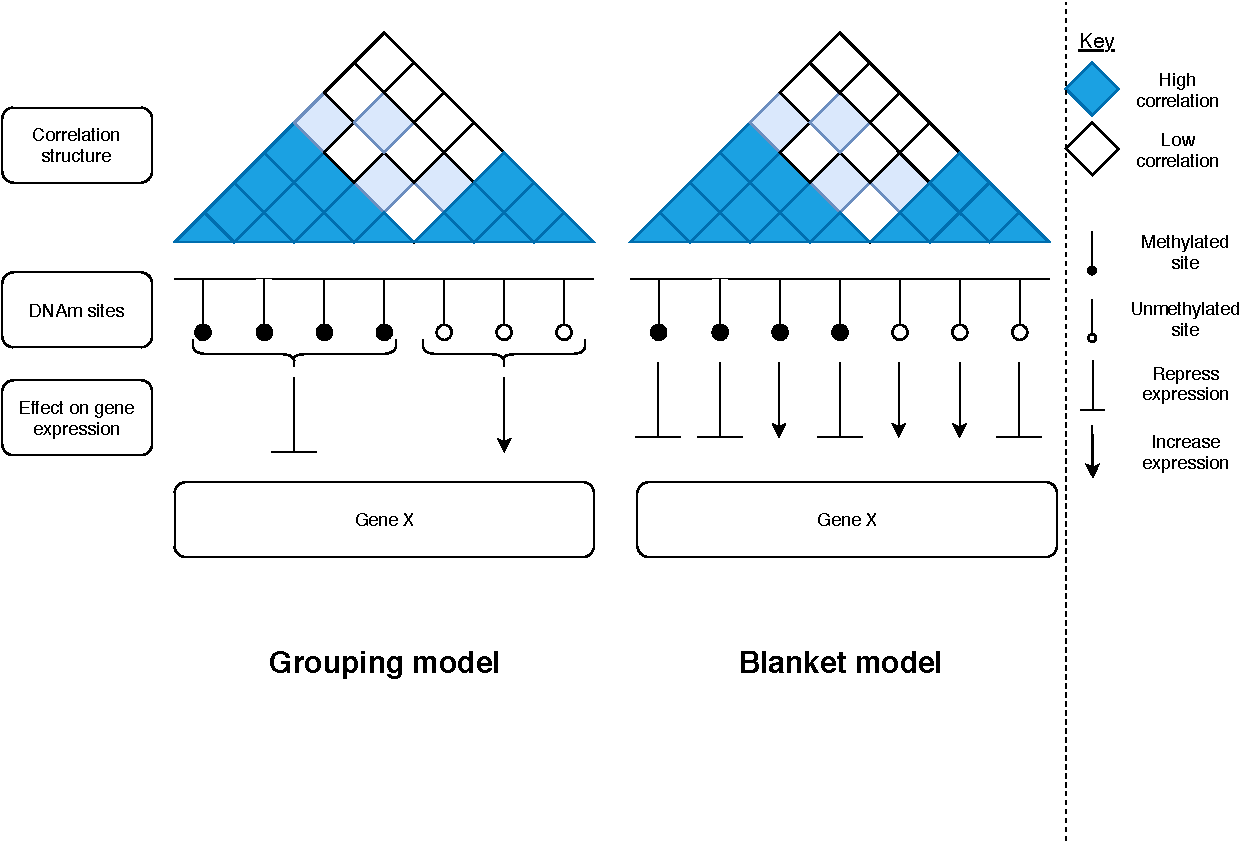
\includegraphics[width=1\linewidth]{figure/05-h2ewas/m2_model_comparison} 

}

\caption{Comparison of the grouping and blanket models in the context of the relationship between DNA methylation and gene expression. Both regions are exactly the same, the only difference is how each model assumes the methylation sites should be treated. The grouping model down-weights the contribution of correlated CpGs, effectively grouping them, and the blanket model assumes each CpG independently associates with a trait. As seen here, the grouping of correlated CpG sites may not be the correct thing to do as some of the sites may be acting independently of their correlated partners).}\label{fig:h2ewas-model-comp}
\end{figure}
\hypertarget{method-05}{%
\section{Method}\label{method-05}}

\hypertarget{study-samples-05}{%
\subsection{Study samples}\label{study-samples-05}}

\hypertarget{methods-alspac-05}{%
\subsubsection{Avon Longitudinal Study of Parents and Children (ALSPAC)}\label{methods-alspac-05}}

All data for the study came from the Avon Longitudinal Study of Parents and Children (ALSPAC) cohort. Pregnant women resident in Avon, UK with expected dates of delivery 1st April 1991 to 31st December 1992 were invited to take part in the study. The initial number of pregnancies enrolled is 14,541 (for these at least one questionnaire has been returned or a ``Children in Focus'' clinic had been attended by 19/07/1999). Of these initial pregnancies, there was a total of 14,676 foetuses, resulting in 14,062 live births and 13,988 children who were alive at 1 year of age. Full details of the cohort has been published previously (125,126). This study uses phenotypic and DNA methylation data from the mothers (N = 940).

Continuous and binary phenotypes measured in mothers were extracted from the cohort. A summary of the phenotypes is present in the Supplementary Material. Please note that the study website contains details of all the data that is available through a fully searchable data dictionary and variable search tool \url{http://www.bristol.ac.uk/alspac/researchers/our-data/}

Phenotype data were extracted using the `alspac' R package (github.com/explodecomputer/alspac) and went through various quality control steps, which are detailed in the Supplementary Material and summarized in Supplementary Figure 1.

All continuous traits were rank-normalised for further analyses. A Shapiro-Wilk test of normality was performed on these rank-normalised traits and for those with some evidence of non-normality (P \textless{} 0.05), we re-examined the distribution of those traits by eye to ensure it was approximately normal. It was found that any non-normality of phenotype distributions corresponded to an inflation of zero values. These traits were removed and overall there were 2408 traits left for analyses. These traits do not necessarily represent independent phenotypes and as such we wanted to prevent correlated traits skewing results. The absolute Pearson's correlation coefficient between each trait was subtracted from one (1 --{[}r{]}). Then traits were greedily selected where 1 --{[}r{]} \textless{} 0.4 with any other trait. This left 400 traits, which consisted of \textasciitilde30\% clinically measured variables (including roughly 50 metabolites and some anthropometric traits), \textasciitilde25\% health related questions (for example ``have you ever had asthma?''), \textasciitilde40\% behavioural and social traits (for example educational attainment variables, use of pesticide, and having pets), and \textasciitilde5\% of traits were related to the partner or child of the participant (for example the employment status of the partner). Phenotypes are presented in Supplementary table 1. Plots showing the correlation between all the phenotypes as well as with just the selected traits can be seen in Supplementary figure 2-3.

Ethical approval for ALSPAC was obtained from the ALSPAC Ethics and Law Committee and from the UK National Health Service Local Research Ethics Committees. Written informed consent was obtained from both the parent/guardian and, after the age of 16, children provided written assent. Consent for biological samples has been collected in accordance with the Human Tissue Act (2004). Informed consent for the use of data collected via questionnaires and clinics was obtained from participants following the recommendations of the ALSPAC Ethics and Law Committee at the time.

\hypertarget{dna-methylation-data-05}{%
\subsection{DNA methylation data}\label{dna-methylation-data-05}}

DNA methylation was measured using the Illumina Infinium HumanMethylation450 (HM450) BeadChip. Before use, the data went through quality control and were normalised separately to the phenotype data. Full details can be found in the Supplementary Material.

DNA methylation data generated from blood collected at a single clinic visit was used for each of the participants.

Probes were excluded if they were present on either of the sex chromosomes, a SNP/control probe, had a detection p value \textless{} 0.05 across over 10\% of samples or were identified as problematic by Zhou et al.~(80). This left 421,693 CpG sites for analyses.

Before analysis a linear regression model was fitted with beta values for methylation (which ranges from 0 (no cytosines methylated) to 1 (all cytosines methylated)) as the outcome against batch variables (plate ID in ALSPAC) modelled as a random effect to help remove the effects of batch in the subsequent analyses.

Cell proportions (CD8+ and CD4+ T cells, B cells, monocytes, natural killer cells, and granulocytes) were estimated using an algorithm proposed by Houseman et al.~(75).

\hypertarget{reml-analysis}{%
\subsection{REML analysis}\label{reml-analysis}}

Using LDAK (163) the relationship between the methylomes (as measured by the HM450 BeadChip) of 940 individuals was estimated by producing a DNA methylation relationship matrix (MRM). This matrix was used as input for the REML analysis to estimate the proportion of a trait's variation that was explained by DNA methylation (h\textsuperscript{2}\textsubscript{EWAS}). Age, the top 10 ancestry principal components, and derived cell proportions were added as covariates to the model.

When producing the MRM, probes were scaled by their observed variance and the weighting of each probe was based on the variance of DNA methylation at that site using the formula below:
\begin{equation}
    f_{j}(1-f_{j})^(\alpha/2)
    \label{eq:mrm-weights}
\end{equation}
where \(f_j(1-f_j)\) is the variance of methylation at CpG \(j\). The higher the alpha value the more weight is given to probes with greater variance; an alpha value of -1 gives equal weight to probes with low and high variance. The alpha value of -0.25 was chosen because previous analysis by Speed et al.~(163) suggested that this value was optimal for measuring h2SNP. Furthermore, it was hypothesised that probes with a greater variance would contribute more to trait variance. As the method was applied to DNA methylation data in this study, sensitivity analyses were conducted. MRMs were created specifying the alpha value at increasing increments of 0.25 from -2 to 0. The association between h\textsuperscript{2}\textsubscript{EWAS} and number of EWAS hits as well as the difference in h\textsuperscript{2}\textsubscript{EWAS} estimates for 10 randomly selected phenotypes was assessed for the varying alpha values.

The mean of the MRM diagonal should be 1 and the variance close to 0, as the diagonal values essentially represent the correlation between an individual's methylome with itself. Although values are expected to vary slightly from 1. For the MRMs it was identified that some diagonal elements were very high (\textgreater{} 2), which caused the diagonal to have a high variance (0.13). To assess whether these values could skew results, we conducted sensitivity analyses removing individuals, with varying diagonal value cutoffs.

Like h2SNP estimates, h\textsuperscript{2}\textsubscript{EWAS} estimates should range from zero to one. If a trait has a true h\textsuperscript{2}\textsubscript{EWAS} value of zero, there is no association between the methylome and that trait, and if h\textsuperscript{2}\textsubscript{EWAS} equals one then DNA methylation has the capacity to completely predict that trait. However, estimation of h\textsuperscript{2}\textsubscript{EWAS} can be fairly imprecise and without constraining the software it's possible to get estimates of h\textsuperscript{2}\textsubscript{EWAS} that are outside 0-1 due to large standard errors. These point estimates have to be erroneous by definition.

Even though the grouping model effectively groups sites together, it is actually likely to increase the number of parameters because without the weightings imposed by this model, the blanket model essentially ignores sites that are not neighbouring others. Therefore, larger standard errors are expected with the grouping model. The grouping model applies a sliding window approach, with windows of 100kb, to capture the correlation between neighbouring sites and weight sites according to the correlation structure of the region. When applying the grouping model, the number of sites that were weighted were 45,863 (out of 421,693) and the number of sites neighbouring any single CpG site ranged from 29 to 28,217.

\hypertarget{generating-genetic-principal-components}{%
\subsection{Generating genetic principal components}\label{generating-genetic-principal-components}}

Ancestry principal components were generated within ALSPAC mothers using PLINK (v1.9). Before analysis, genetic data went through quality control and were imputed, full details can be found in the Supplementary Material. After quality control and imputation, independent SNPs (r2 \textless{} 0.01) were used to calculate the top 10 ancestry principal components.

\hypertarget{methods-ewas-05}{%
\subsection{Epigenome-wide association studies}\label{methods-ewas-05}}

EWAS were conducted for 400 selected traits (see Study Samples section for selection process) within the ALSPAC cohort. For all traits, linear regression models were fitted with beta values of DNA methylation as the outcome and the phenotype as the exposure. Covariates included age, the top 10 ancestry principal components and cell proportions.

\hypertarget{methods-h2ewas-dmp}{%
\subsection{\texorpdfstring{Association between h\textsuperscript{2}\textsubscript{EWAS} and epigenome-wide association studies results}{Association between h2EWAS and epigenome-wide association studies results}}\label{methods-h2ewas-dmp}}

DMPs were extracted from the EWAS at P value thresholds ranging from 10-3 to 10-7. It was assessed whether h\textsuperscript{2}\textsubscript{EWAS} could predict that the number of identified DMPs in an EWAS was greater than number of DMPs expected to be identified at a given P threshold defined as the number of sites tested multiplied by the threshold. The traits were also ``pruned'' in the same way as described above, to prevent including overly correlated traits and biasing results. The sensitivity and specificity of this prediction was calculated and a receiver operating characteristic (ROC) curve was plotted. At p-value thresholds of 10-6.5 and 10-7 there were too few EWAS hits, so these were removed from the analysis.

The association between the number of DMPs identified at P \textless{} 1x10-5 and h\textsuperscript{2}\textsubscript{EWAS} values was assessed using a negative binomial hurdle model with the number of DMPs identified fitted as the outcome and h\textsuperscript{2}\textsubscript{EWAS} as the exposure. The negative binomial hurdle Poisson regression model results are twofold. The first of which assesses whether there is an association between the binary trait of whether a DMP was identified by EWAS and h\textsuperscript{2}\textsubscript{EWAS}. The second is a zero-truncated model, i.e.~the zero values are removed from the model and the association between number of DMPs and h\textsuperscript{2}\textsubscript{EWAS} is assessed.

The same method was applied to estimate the association between the number of SNPs identified in GWAS at P \textless{} 5x10-8 and h2SNP. SNPs associated with 485 traits in UK Biobank (see Supplementary Methods for sample information and phenotype selection) were extracted using the IEU Open GWAS Database (92). The h2SNP estimates were extracted from \url{http://www.nealelab.is/uk-biobank/}.

All analyses were conducted in R (version 3.3.3) or using the command line software LDAK (163), GCTA (164), and PLINK (165). For the EWAS analyses, the meffil R package was used (166). A one-sided P value was used to assess if the h\textsuperscript{2}\textsubscript{EWAS} for a trait was \textgreater{} 0, and two-sided P values were used for everything else.

\hypertarget{data-availability-05}{%
\subsection{Data availability}\label{data-availability-05}}

Code used to perform analyses can be found here: github.com/thomasbattram/ereml

The full EWAS summary statistics of each of the 400 EWAS are available via Zenodo here

\hypertarget{results-05}{%
\section{Results}\label{results-05}}

A flowchart showing our study design and giving a summary of the results is shown in \textbf{Figure \ref{fig:h2ewas-study-design}}.


\begin{figure}

{\centering 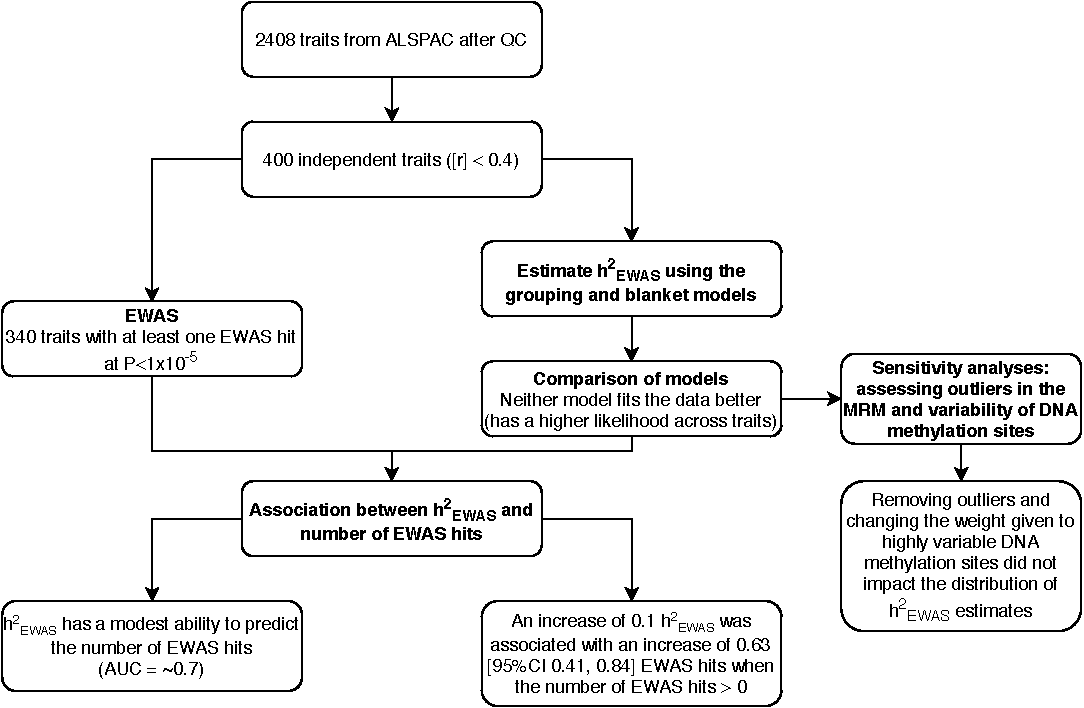
\includegraphics[width=1\linewidth]{figure/05-h2ewas/m2_workflow} 

}

\caption{Study design with a summary of the results. ALSPAC = Avon Longitudinal Study of Parents and Children, QC = quality control, EWAS = epigenome-wide association study, MRM = methylation relationship matrix, AUC = area under curve.}\label{fig:h2ewas-study-design}
\end{figure}
\hypertarget{estimating-h2ewas}{%
\subsection{Estimating the proportion of phenotypic variance associated with DNA methylation}\label{estimating-h2ewas}}

We used two models to estimate the total contribution of all DNA methylation sites to the variation (h\textsuperscript{2}\textsubscript{EWAS}) for each of 400 traits within 940 individuals. The mean for both models was zero with ranges of -0.4 to 0.4 and -0.5 to 0.4 for the blanket and grouping models respectively \textbf{Figure \ref{fig:h2ewas-estimates}}. The estimates were imprecise with the mean standard error was 0.03 and 0.05 for the blanket and grouping models respectively. The trait with the greatest evidence for h\textsuperscript{2}\textsubscript{EWAS} estimates being above zero was having smoked cigarettes regularly (FDR-corrected P = 0.06 and 0.10 for the blanket and grouping models respectively). The correlation between the h\textsuperscript{2}\textsubscript{EWAS} estimates of the two models was 0.47 and there was evidence that on average the estimates of the grouping model were higher (Paired t-test P = 1.8x10-5, \textbf{Figure \ref{fig:h2ewas-estimates}}), but the mean difference between estimates was only 0.018.

There was little evidence that either of the models fit the data better (had higher likelihoods) across the 400 traits tested (difference in median likelihoods = 0.19, Wilcoxon's paired ranked sum test P = 0.73). Further, the majority of h\textsuperscript{2}\textsubscript{EWAS} estimate differences between the traits were small.


\begin{figure}

{\centering 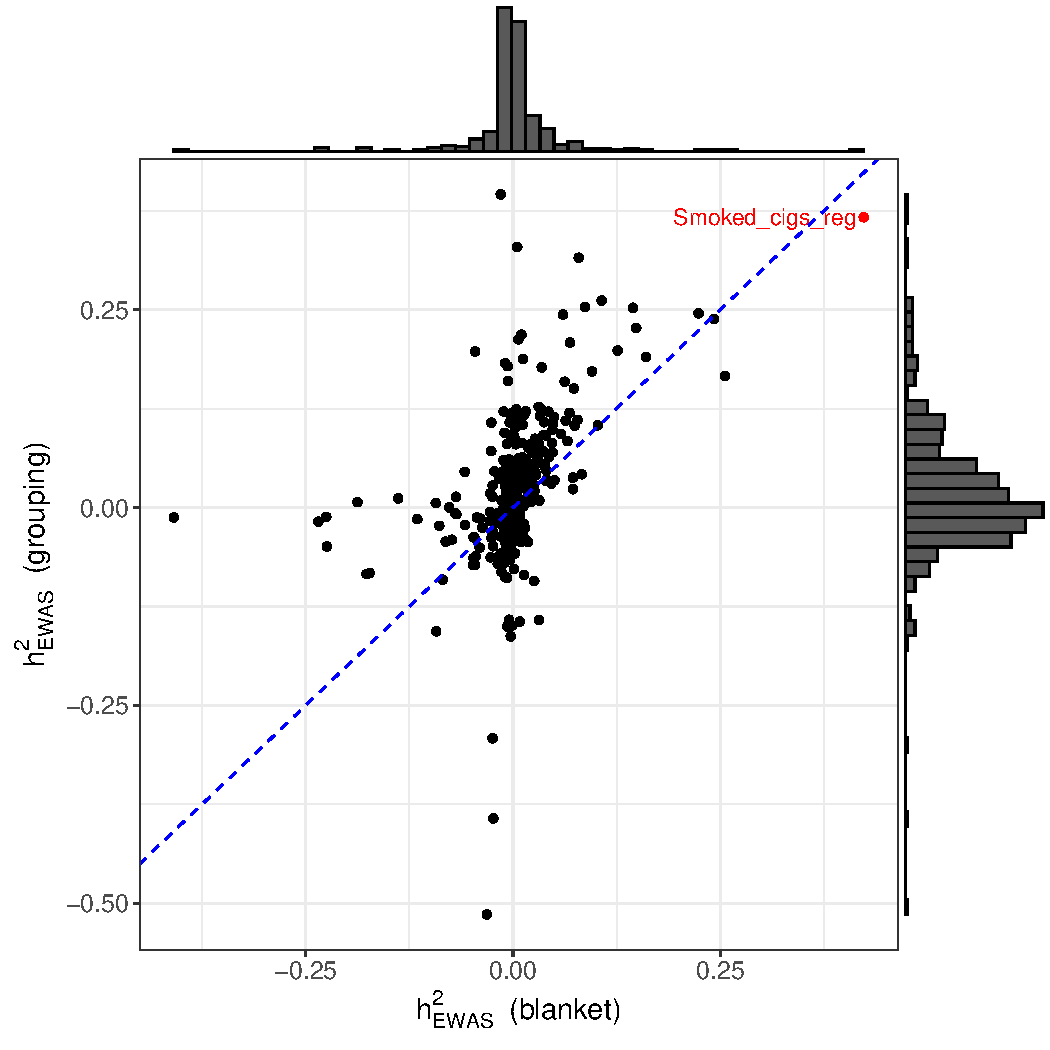
\includegraphics[width=1\linewidth]{figure/05-h2ewas/model_m2_comparison} 

}

\caption{A comparison of h\textsuperscript{2}\textsubscript{EWAS} estimates given by applying REML using the blanket and grouping models across 400 traits. The blue dashed line is at x=y. Values with h\textsuperscript{2}\textsubscript{EWAS} lower than 0 are due to imprecision in h\textsuperscript{2}\textsubscript{EWAS} estimates as the true estimate cannot be negative. Smoked\_cigs\_reg = smoked cigarettes regularly. The h\textsuperscript{2}\textsubscript{EWAS} of this phenotype has the greatest evidence for being above 0 for both the blanket and grouping model (Uncorrected P = 1.44x10-4 and P = 2.61x10-4, respectively).}\label{fig:h2ewas-estimates}
\end{figure}
\hypertarget{results-sensitivity-analyses-05}{%
\subsection{Sensitivity analyses when estimating the proportion of phenotypic variance associated with DNA methylation}\label{results-sensitivity-analyses-05}}

After examination of the MRMs required to produce the h\textsuperscript{2}\textsubscript{EWAS} estimates, we found that for both the blanket and grouping model we observed some unexpected values: 96 diagonal elements had values over 1.5 when using the blanket model, with the maximum value being 3.562. When assessing the impact of these potential outliers in the MRM to results we found that the median and range of h\textsuperscript{2}\textsubscript{EWAS} estimates varied little (Supplementary figure 4). The likelihood of the models tended to be greater as more outliers were removed (lower threshold for classing a diagonal element as an outlier), but it still didn't vary much (Supplementary figure 5).

The weight of predictors used to produce the MRMs was also examined. As more weight was given to sites where methylation variation was greater (increasing alpha value) the h\textsuperscript{2}\textsubscript{EWAS} estimates were slightly higher (Supplementary figure 6). However, the likelihood tended to remain the same, the median likelihood had a range of 2 across the alpha values (Supplementary figure 7).

Results of sensitivity analyses are summarised in Supplementary table 2 and 3.

\hypertarget{results-ewas-analyses-05}{%
\subsection{EWAS analyses}\label{results-ewas-analyses-05}}

In order to assess the association between h\textsuperscript{2}\textsubscript{EWAS} and EWAS results, we performed EWAS of 400 traits. No associations were found at the strict P value cutoff of P \textless{} 2.5x10-10 (conventional EWAS P-value threshold, 1x10-7, divided by the number of traits, 400). A total of 29 associations between traits and CpGs were identified at the conventional EWAS P value cutoff -- P \textless{} 1x10-7. Of the traits tested, 16 had at least one EWAS hit, with the maximum number of CpGs associated with a trait being 13 (smoked cigarettes regularly). As there were so few traits with any identified hits, we took forward results from the lenient P value threshold of P \textless{} 1x10-5, at which 340 traits had at least one EWAS hit. Supplementary table 4 shows each trait and the number of differentially methylated positions identified at varying p-value thresholds.

As the distributions of hit count data was heavily right skewed with an inflation at 0 and 1 (Supplementary figure 8), to test the association between h\textsuperscript{2}\textsubscript{EWAS} and number of DMPs we opted to test goodness of fit for variations of Poisson models. Of the 6 models tested, the negative binomial hurdle Poisson regression model fit the data best, full results can be found in Supplementary table 5. We found there was some evidence for an association between number of EWAS hits and h\textsuperscript{2}\textsubscript{EWAS} (\textbf{Figure \ref{fig:dmps-and-h2ewas}}). There was some evidence of association between the presence of DMPs and h\textsuperscript{2}\textsubscript{EWAS} (beta = 6.2, {[}95\%CI 2.5, 10{]}) as well as some evidence of an association between number of DMPs (when the number is above 0) and h\textsuperscript{2}\textsubscript{EWAS} (mean increase of 0.63, {[}95\%CI 0.41, 0.84{]} DMPs when h\textsuperscript{2}\textsubscript{EWAS} increases by 0.1). Applying the same method to GWAS data we found evidence that the presence of identified SNPs associated with h2SNP (beta = 21.9 {[}95\%CI 19.6, 24.1{]})and the association between number of SNPs identified (when the number is above 0) and h2SNP (mean increase of 1.5, {[}95\%CI 0.93, 2.5{]} SNPs when h2SNP increases by 0.1).


\begin{figure}

{\centering 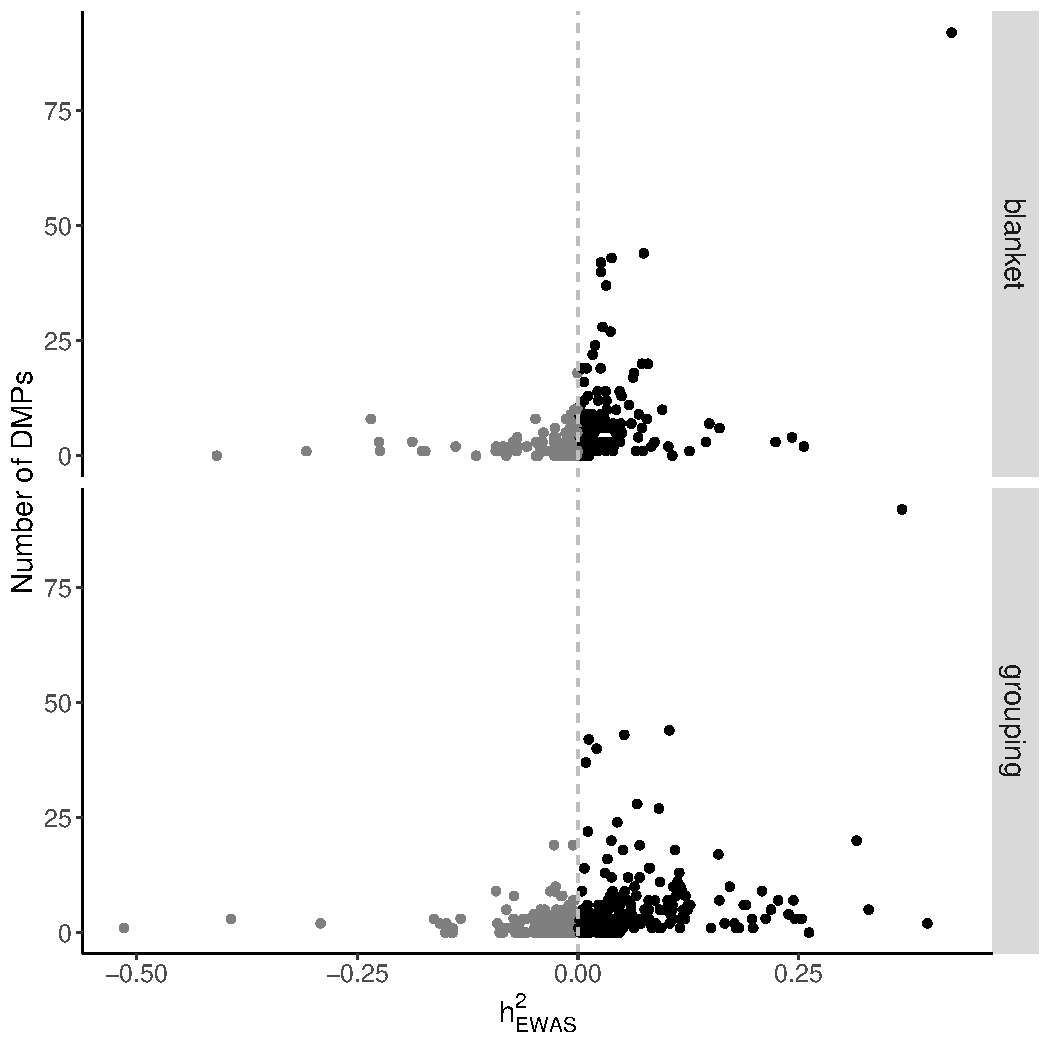
\includegraphics[width=1\linewidth]{figure/05-h2ewas/m2_hit_count_scatter_p5_test} 

}

\caption{Association between h\textsuperscript{2}\textsubscript{EWAS} and number of DMPs identified in EWAS. The correlation between DNA methylation and the variance of traits (h\textsuperscript{2}\textsubscript{EWAS}) was calculated using REML analysis using the blanket and grouping models. EWAS were conducted on all the same traits and the distribution of the number of DMPs identified at P \textless{} 1x10-5 and h\textsuperscript{2}\textsubscript{EWAS} are plotted above. Any traits where the h\textsuperscript{2}\textsubscript{EWAS} estimate is below 0 are coloured grey. The true h\textsuperscript{2}\textsubscript{EWAS} value of a trait cannot be negative, but sample sizes in this analysis are small so the estimates are imprecise.}\label{fig:dmps-and-h2ewas}
\end{figure}
The ability of h\textsuperscript{2}\textsubscript{EWAS} estimated by both models to predict whether the number of DMPs identified was greater than expected was assessed at varying P value thresholds. ROC curves were produced and the area under the curve (AUC) ranged from 0.65 and 0.67 at P \textless{} 1e-6 to 0.79 and 0.71 at P \textless{} 1e-3 for the blanket and grouping models respectively and the predictive ability remained fairly stable as the threshold increased (\textbf{Figure \ref{fig:h2ewas-dmp-roc-curve}}).


\begin{figure}

{\centering 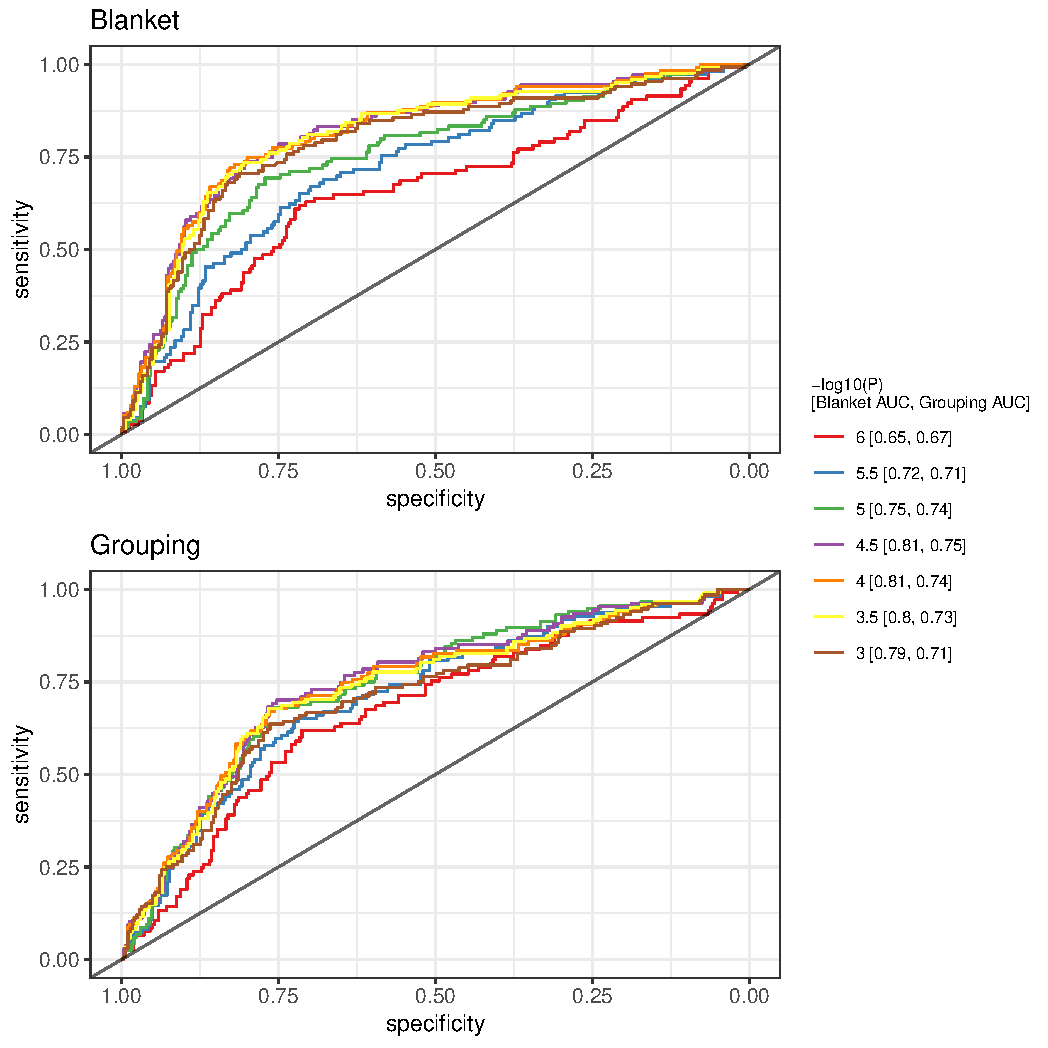
\includegraphics[width=1\linewidth]{figure/05-h2ewas/roc_plot} 

}

\caption{Association between h\textsuperscript{2}\textsubscript{EWAS} and number of DMPs identified in EWAS. The correlation between DNA methylation and the variance of traits (h\textsuperscript{2}\textsubscript{EWAS}) was calculated using REML analysis using the blanket and grouping models. EWAS were conducted on all the same traits and the distribution of the number of DMPs identified at P \textless{} 1x10-5 and h\textsuperscript{2}\textsubscript{EWAS} are plotted above. Any traits where the h\textsuperscript{2}\textsubscript{EWAS} estimate is below 0 are coloured grey. The true h\textsuperscript{2}\textsubscript{EWAS} value of a trait cannot be negative, but sample sizes in this analysis are small so the estimates are imprecise.}\label{fig:h2ewas-dmp-roc-curve}
\end{figure}
\hypertarget{discussion-05}{%
\section{Discussion}\label{discussion-05}}

The global contribution of DNA methylation to complex trait variance can inform researchers of how to design future studies that seek to discover new DNA methylation sites associated with their trait of interest. In this manuscript we apply methods designed to estimate the predictive capacity of variants across a SNP-chip (h2SNP), to DNA methylation data measured in blood with the HM450 BeadChip across 400 independent traits, giving a distribution of the contribution of all sites typically measured in EWAS to complex trait variance. Although sample size was too small to reliably estimate h\textsuperscript{2}\textsubscript{EWAS} for any one trait, the distribution of estimates suggest little complex trait variation is captured by DNA methylation at the sites measured and h\textsuperscript{2}\textsubscript{EWAS} may be a good measure to identify traits for which EWAS will yield associations.

\hypertarget{estimation-of-h2ewas}{%
\subsection{\texorpdfstring{Estimation of h\textsuperscript{2}\textsubscript{EWAS}}{Estimation of h2EWAS}}\label{estimation-of-h2ewas}}

The true h\textsuperscript{2}\textsubscript{EWAS} of a trait gives the total predictive capacity of DNA methylation for that trait, which is equivalent to the proportion of that trait's total variance that is associated with changes in DNA methylation. Knowing this information can help design future EWAS studies. A low value of h\textsuperscript{2}\textsubscript{EWAS} doesn't necessarily mean there is little correlation between DNA methylation and a trait, it could transpire that unmeasured sites contribute more to the association. It is important to remember that roughly 1.5\% of CpG sites are targeted by the HM450 BeadChip and DNA can be methylated elsewhere (not at cytosine bases). Therefore, whole genome bisulphite sequencing, or a similar technique, may show that the variance of complex traits captured by DNA methylation is far higher. Furthermore, even if h\textsuperscript{2}\textsubscript{EWAS} is low and the sites discovered already do not explain all of the h\textsuperscript{2}\textsubscript{EWAS} estimate, there may still be value in increasing sample size to identify more DMPs as well as increase the precision of h\textsuperscript{2}\textsubscript{EWAS} estimates. DMPs discovered may not be highly correlated with a trait, but this doesn't mean the potential biological information gained isn't valuable. For example, if a change in a the levels of protein X has a large effect on a trait and change in DNA methylation has a small effect on the levels of protein X, then the effect of that DNA methylation change on the trait will be small, but identifying that DMP could lead to discovering the importance of the protein. Another thing to consider is that DNA methylation is tissue and cell specific. This means, that h\textsuperscript{2}\textsubscript{EWAS} may vary a lot depending on what tissue the methylation is measured in.

The true underlying genetic architecture of complex traits is still unknown, and therefore it is difficult to know the appropriate model to choose when estimating the contribution of all measured SNPs to phenotypic variance amongst unrelated individuals and arguments for each model depending on this underlying genetic architecture are still being put forward (163), (167--169), thus the attempts made in this study to re-purpose genomic REML are likely to suffer the same flaws that are trying to be overcome in genetic data. With this in mind, in addition to the imprecise estimates of h\textsuperscript{2}\textsubscript{EWAS} presented here (due to the small sample sizes of available data), we believe that individual trait h\textsuperscript{2}\textsubscript{EWAS} values should be treated with caution. This doesn't exclude the possibility that estimating h\textsuperscript{2}\textsubscript{EWAS} may be useful and other methods are already being developed to measure the association between DNA methylation at all sites and complex traits (123).

\hypertarget{future-ewas-05}{%
\subsection{Future EWAS}\label{future-ewas-05}}

Heritability estimates from family-based studies gave an a priori justification for the pursuit of gene mapping endeavours that eventually gave rise to GWAS, as they demonstrated variation in complex traits had a substantial genetic component. However, the evidence DNA methylation contributed to trait variation was not ascertained before EWAS were first conducted. To justify collecting more samples and continuing with EWAS research in the current vein, methods such as the one presented in this study should be used to show DNA methylation does substantially contribute to trait variance.

It has become clear from the GWAS era of genetics, that for complex traits, such as coronary artery disease, many common genetic variants with small effects make up the genetic component of the trait (170,171). This suggests a large number of molecular pathways contribute to these traits. DNA methylation at CpGs is heritable (3,145), thus it would be expected that the DNA methylation architecture of a trait will somewhat reflect the genetic architecture of the trait, although this has not been empirically tested.

Despite uncertainty of h\textsuperscript{2}\textsubscript{EWAS} estimates for individual traits, we show h\textsuperscript{2}\textsubscript{EWAS} has a modest ability to predict whether the number of EWAS hits will be greater than expected by chance at a given P value threshold. This predictive ability remained stable as the P value threshold for detection increased from P \textless{} 1x10-6 to P \textless{} 1x10-3. These results suggest that increasing sample sizes for traits which truly associate with DNA methylation should result in the discovery of more DMPs. Furthermore, these results support a model for which small changes in methylation at many CpGs across the genome are related to complex traits.

\hypertarget{contribution-of-individual-cpg-sites}{%
\subsection{Contributions of individual CpG sites}\label{contribution-of-individual-cpg-sites}}

The original model for measuring h2SNP assumed all genetic variants contributed the same effect on a trait (95), Speed et al.~offered an alternative model assuming a different underlying genetic architecture, whereby genetic variants in regions of high LD contributed less to the variance of a trait than more independent variants. Both groups have shown that the performance of the models depend on the alignment of the trait's architecture with the models' underlying assumptions. Previous literature has suggested that it is the methylation across groups of CpGs that may affect how other molecules interact with DNA and influence cellular functions such as gene expression (18). Furthermore, CpGs are not randomly distributed throughout the genome -- many exist in close proximity within ``islands'' or other regions, suggesting that grouping of the CpGs may have functionality. However, the most common method used in EWAS is to treat CpG sites as independent. Here, the models proposed by Speed et al.~(the grouping model) and Yang et al.~(the blanket model), when estimating h\textsuperscript{2}\textsubscript{EWAS} were tested across 400 traits. The model fit the data better (had a higher likelihood) 207 times for the blanket model and 193 times for the grouping model. Thus for almost half the traits treating DNA methylation sites as independent seems to be preferable and even though there is correlation between CpG sites, which allows them to be grouped, it might be that in some groups of correlated sites, individual sites within the group contribute separately to trait variance.

It's important to note that the grouping method takes into account correlation between CpGs within 100Kb of each other. Differential methylation at CpG sites may be correlated for a variety of biological reasons, for example, CpGs lying within a transcription factor binding site will be regulated together, but also, they will be correlated with CpGs that lie in other binding sites for that same transcription factor and these may be many megabases away. This is relevant to the relationship between DNA methylation and complex traits because transcription factor regulation might be the link between complex traits and DNA methylation. Even though grouping CpG sites might yet be the best way to model the relationship between DNA methylation and complex traits, the optimum way to group sites is unknown and will likely change depending on the trait of interest.

\hypertarget{limitations-05}{%
\subsection{Limitations}\label{limitations-05}}

The main limitation of the study is the small sample size (N = 940) to estimate the h\textsuperscript{2}\textsubscript{EWAS}. This meant the precision of our h\textsuperscript{2}\textsubscript{EWAS} estimates were very low and so our power to assess their ability to predict number of DMPs and find individual trait h\textsuperscript{2}\textsubscript{EWAS} values was low. To circumvent this problem, we assess trends across multiple traits and do not make strong conclusions for any one trait.

As mentioned previously the HM450 BeadChip captures a small percentage of the total DNA methylome and h\textsuperscript{2}\textsubscript{EWAS} estimates will likely vary upon assaying more DNA methylation sites. Furthermore, when measuring more sites, it might be that one of the models fits the data better. Nevertheless, the results of this study can still give evidence towards the hypothesis that differential methylation at many sites across the genome each contribute minimally to the overall association between the methylome and a complex trait.

Unlike germline genetic variants, there is intra-individual (between tissue and over time) DNA methylation variation (1,63). Thus, it is to be expected that the variation of h\textsuperscript{2}\textsubscript{EWAS} estimates across traits is partly a product of the tissue and timepoint of choice. However, within the tissue biologically pertinent to the complex trait of interest, the number of pathways that associate with variation in that trait is likely to remain high, for example there are many processes affecting, or affected by, cancer development (172). Thus, it would still be expected that differential methylation at many CpG sites each associate with a trait, but the effect sizes are small. The same can be said when estimating h\textsuperscript{2}\textsubscript{EWAS} at various timepoints.

Estimates of h\textsuperscript{2}\textsubscript{EWAS} will be a product of their environment and genetic makeup of the participants it's measured in. Therefore, the results here may vary by population and by sex. However, participants used in this study are considered to be representative of the larger ALSPAC cohort (173), which is itself considered to be representative of a large majority of women from the UK and potentially other high-income countries (125). This suggests the results will be generalisable to a large group of samples for which EWAS are conducted, but replication in these samples as well as in different populations would provide greater confidence in the generalisability of the results.

A wide range of complex traits was used in the analysis, but there are some notable absences. Rarer diseases and diseases that predominantly impact the elderly are not present in this study. The results presented here cannot be generalised to those traits.

The factors important for the correlation structure of DNA methylation data are less known than those for linkage disequilibrium structure of genetic variants. Therefore, when applying models, such as the grouping model here, that aim to account for correlation of neighbouring DNA methylation sites, we may be missing some of the important structure captured for example by trans-correlations (over 1Mb). A model that estimates h\textsuperscript{2}\textsubscript{EWAS} by incorporating all of the underlying correlation of DNA methylation data may therefore outperform both models tested here.

\hypertarget{conclusion-05}{%
\section{Conclusion}\label{conclusion-05}}

Overall, the number of traits with good evidence for h\textsuperscript{2}\textsubscript{EWAS} \textgreater{} 0 was low (only smoking behaviour met the threshold of FDR \textless{} 0.1) and mean h\textsuperscript{2}\textsubscript{EWAS} value across both models was roughly 0, suggesting that for many traits DNA methylation variation as measured on the HM450 BeadChip in blood is of little relevance. However, these estimates varied greatly and therefore DNA methylation measured in this way will likely have relevance for some traits, for example smoking cigarettes regularly. Further, these estimates were correlated with the number of DMPs identified, suggesting that for traits whose variance associates with DNA methylation then increasing sample size will yield an increase in the number of CpGs identified in EWAS. We also provide evidence that there is value in assessing individual CpG-trait associations as opposed to groups of correlated CpG sites within 100Kb. However, this does not preclude the possibility that a more complex model of CpG site correlation may provide a better fit.

\hypertarget{ewas-gwas-comp-chapter}{%
\chapter{EWAS-GWAS comparison}\label{ewas-gwas-comp-chapter}}

\hypertarget{dnam-lung-cancer-mr}{%
\chapter{Appraising the causal relevance of DNA methylation for risk of lung cancer}\label{dnam-lung-cancer-mr}}

\hypertarget{abstract-07}{%
\section{Abstract}\label{abstract-07}}

\hypertarget{abstract-background-07}{%
\subsection{Background}\label{abstract-background-07}}

DNA methylation changes in peripheral blood have recently been identified in relation to lung cancer risk. Some of these changes have been suggested to mediate part of the effect of smoking on lung cancer. However, limitations with conventional mediation analyses mean that the causal nature of these methylation changes has yet to be fully elucidated.

\hypertarget{abstract-methods-07}{%
\subsection{Methods}\label{abstract-methods-07}}

We first performed a meta-analysis of four epigenome-wide association studies (EWAS) of lung cancer (918 cases, 918 controls). Next, we conducted a two-sample Mendelian randomization analysis, using genetic instruments for methylation at CpG sites identified in the EWAS meta-analysis, and 29,863 cases and 55,586 controls from the TRICL-ILCCO lung cancer consortium, to appraise the possible causal role of methylation at these sites on lung cancer.

\hypertarget{abstract-results-07}{%
\subsection{Results}\label{abstract-results-07}}

16 CpG sites were identified from the EWAS meta-analysis (FDR \textless{} 0.05), 14 of which we could identify genetic instruments for. Mendelian randomization provided little evidence that DNA methylation in peripheral blood at the 14 CpG sites play a causal role in lung cancer development (FDR \textgreater{} 0.05), including for cg05575921-\emph{AHRR} where methylation is strongly associated with both smoke exposure and lung cancer risk.

\hypertarget{abstract-conclusions-07}{%
\subsection{Conclusions}\label{abstract-conclusions-07}}

The results contrast with previous observational and mediation analysis, which have made strong claims regarding the causal role of DNA methylation. Thus, previous suggestions of a mediating role of methylation at sites identified in peripheral blood, such as cg05575921-\emph{AHRR}, could be unfounded. However, this study does not preclude the possibility that differential DNA methylation at other sites is causally involved in lung cancer development, especially within lung tissue.

\hypertarget{introduction-07}{%
\section{Introduction}\label{introduction-07}}

Lung cancer is the most common cause of cancer-related death worldwide (174). Several DNA methylation changes have been recently identified in relation to lung cancer risk (121,175,176). Given the plasticity of epigenetic markers, any DNA methylation changes that are causally linked to lung cancer are potentially appealing targets for intervention (177,178). However, these epigenetic markers are sensitive to reverse causation, being affected by cancer processes (178), and are also prone to confounding, for example by socio-economic and lifestyle factors {[}(179); Elliott2014{]}.

One CpG site, cg05575921 within the aryl hydrocarbon receptor repressor (\emph{AHRR}) gene, has been consistently replicated in relation to both smoking (65) and lung cancer (101,121,175) and functional evidence suggests that this region could be causally involved in lung cancer (138). However, the observed association between methylation and lung cancer might simply reflect separate effects of smoking on lung cancer and DNA methylation, i.e.~the association may be a result of confounding (104), including residual confounding after adjustment for self-reported smoking behaviour (180,181). Furthermore, recent epigenome-wide association studies (EWAS) for lung cancer have revealed additional CpG sites which may be causally implicated in development of the disease (121,175).

Mendelian randomization (MR) uses genetic variants associated with modifiable factors as instruments to infer causality between the modifiable factor and outcome, overcoming most unmeasured or residual confounding and reverse causation (89,90). In order to infer causality, three core assumptions of MR should be met: 1) The instrument is associated with the exposure, 2) The instrument is not associated with any confounders, 3) The instrument is associated with the outcome only through the exposure. MR may be adapted to the setting of DNA methylation (112,173,182) with the use of single nucleotide polymorphisms (SNPs) that correlate with methylation of CpG sites, known as methylation quantitative trait loci (mQTLs) (3).

In this study, we performed a meta-analysis of four lung cancer EWAS (918 case-control pairs) from prospective cohort studies to identify CpG sites associated with lung cancer risk and applied MR to investigate whether the observed DNA methylation changes at these sites are causally linked to lung cancer.

In this chapter, Dr Rebecca Richmond performed analysis in the CCHS cohort (see section \protect\hyperlink{potential-causal-effect-of-ahrr-methylation-on-lung-cancer-risk-one-sample-mr}{Potential causal effect of \emph{AHRR} methylation on lung cancer risk: one sample MR} of the results) and contributed to writing the introduction and discussion. I completed all the analysis and wrote each section except the methods and results sections for which I did not complete the analysis.

\hypertarget{methods-07}{%
\section{Methods}\label{methods-07}}

\hypertarget{ewas-study-details}{%
\subsection{EWAS study details}\label{ewas-study-details}}

A meta-analysis of four lung cancer case-control EWAS was conducted to identify DNA methlyation sites associated with lung cancer. DNA methylation in each EWAS was assessed using the Illumina Infinium® HumanMethylation450 BeadChip. All EWAS are nested within prospective cohorts that measured DNA methylation in peripheral blood samples before diagnosis: EPIC-Italy (185 case-control pairs), Melbourne Collaborative Cohort Study (MCCS) (367 case-control pairs), Norwegian Women and Cancer (NOWAC) (132 case-control pairs) and the Northern Sweden Health and Disease Study (NSHDS) (234 case-control pairs). Study populations, laboratory methods, data pre-processing and quality control methods have been described in detail elsewhere (121) 3 and are outlined below.

At the various laboratory sites, samples were distributed into 96-well plates and processed in chips of 12 arrays (8 chips per plate) with case-control pairs arranged randomly on the same chip. Methylation data were pre-processed and normalized in each study, and probe filtering was performed as previously described (121), leaving 465,886 CpGs suitable for the analysis in EPIC-Italy, 485,330 CpGs in MCCS, 450,890 CpGs in NOWAC and 482,867 CpGs in NSHDS.

\hypertarget{european-prospective-investigation-into-cancer-and-nutrition-italy-epic-italy}{%
\subsubsection{European Prospective Investigation into Cancer and Nutrition-Italy (EPIC-Italy)}\label{european-prospective-investigation-into-cancer-and-nutrition-italy-epic-italy}}

EPIC-Italy includes 47,749 volunteers (32,579 women) aged 35--70 years at the time of recruitment (1992--1998). Anthropometric measurements and lifestyle variables including detailed information on smoking history were collected at recruitment through standardized questionnaires, together with a blood sample. Within EPIC-Italy we conducted a nested case-control study utilizing incident cases diagnosed within follow-up and healthy controls individually matched to cases by gender, date of birth (±5 years), date of inclusion in the study and study centre. Analysis was performed for 185 incident cases diagnosed within follow-up and matched controls. Laboratory procedures were carried out at the Human Genetics Foundation (Turin, Italy) and DNA extracted from buffy coats as previously described (121). All participants signed an informed consent form, and the ethical review boards of the International Agency for Research on Cancer and of each local participating centre approved the study protocol.

\hypertarget{melbourne-collaborative-cohort-study-mccs}{%
\subsubsection{Melbourne Collaborative Cohort Study (MCCS)}\label{melbourne-collaborative-cohort-study-mccs}}

The MCCS is a prospective cohort study of 41,514 volunteers (24,469 women) aged between 27 and 76 years at baseline (1990-1994). At baseline attendance, participants completed questionnaires that measured demographic characteristics and lifestyle factors. Height and weight were directly measured, and a blood sample was collected and stored. Incident cases of lung cancer were identified through linkage with the State and National Cancer Registries during follow-up up to the end of 2011. The MCCS sample included 367 cases and 367 matched controls selected from MCCS participants who were lung cancer free at the age of diagnosis of the matching case (density sampling). Matching variables included gender, date of blood collection (within 6 months), date of birth (within 1 year), country of birth (Australia and UK versus Southern Europe), type of biospecimen (lymphocyte, buffy coat and dried blood spot) and smoking status (never smokers; short-term former smokers: quitting smoking less than 10 years before blood draw; long-term former smokers: quitting smoking 10 years or more before blood draw; current light smokers: less than 15 cigarettes per day at blood draw; and current heavy smokers: 15 cigarettes or more at blood draw). For the MCCS, laboratory procedures were carried out at the Genetic Epidemiology Laboratory, the University of Melbourne according to manufacturers' protocols. DNA extraction from lymphocytes and buffy coats was performed as previously described (121). The Cancer Council Victoria's Human Research Ethics Committee approved the study protocol. Subjects gave written consent to participate and for the investigators to obtain access to their medical records.

\hypertarget{norwegian-women-and-cancer-nowac}{%
\subsubsection{Norwegian Women and Cancer (NOWAC)}\label{norwegian-women-and-cancer-nowac}}

The biobank of the NOWAC cohort was established in the years 2003-2006. Those who filled in an eight-page questionnaire and accepted the invitation to donate blood were sent blood drawing equipment together with a two-page epidemiological questionnaire. Around 50 000 women returned two tubes of blood to the Institute of Community Medicine at UiT The Arctic University of Norway and data linkage to the National Cancer Registry of Norway was performed. During follow-up to the end of 2011, 132 eligible cases of lung cancer were identified and were used for the EWAS. For each case, one control with an available blood sample was selected and matched on time since blood sampling and year of birth in order to control for effects of storage time and ageing. The cases and the controls were processed together for all laboratory procedures in order to reduce any batch effect. Laboratory procedures were carried out at the Human Genetics Foundation (Turin, Italy). DNA extraction from buffy coats was performed as previously described (121). All participants gave informed consent. The study was approved by the Regional Committee for Medical and Health Research Ethics in North Norway. Data storage and linkage was approved by the Norwegian Data Inspectorate.

\hypertarget{northern-sweden-health-and-disease-study-nshds}{%
\subsubsection{Northern Sweden Health and Disease Study (NSHDS)}\label{northern-sweden-health-and-disease-study-nshds}}

NSHDS is an ongoing prospective cohort and intervention study intended for health promotion of the population of Västerbotten County in northern Sweden. All residents were invited to participate by attending a health check-up at their local health care centre at 40, 50 and 60 years of age. At the health check-up, participants were asked to complete a self-administered questionnaire covering various factors such as education, smoking habits, physical activity and diet. In addition, height and weight were measured and participants were asked to donate a blood sample. Incident lung cancer cases were identified through linkage to the regional cancer registry. One control was chosen at random for each lung cancer case from appropriate risk sets consisting of all cohort members alive and free of cancer (except non-melanoma skin cancer) at the time of diagnosis of the index case. Matching criteria were the same as for the MCCS except there was no matching for type of biospecimens as DNA was extracted from whole blood for all samples. After quality control, a total of 234 incident lung cancer cases and 234 individually matched controls were available for this analysis. Laboratory procedures for NSHDS were carried out at two sites. DNA extraction from the buffy coat was conducted at Umeå University, Sweden, as previously described. Illumina Infinium HumanMethylation450 BeadChip analysis was conducted at the ALSPAC/IEU Laboratory at the University of Bristol. All study subjects provided written informed consent at time of the recruitment into the NSHDS.

\hypertarget{methods-ewas-meta-analysis}{%
\subsection{EWAS Meta-analysis}\label{methods-ewas-meta-analysis}}

To quantify the association between the methylation level at each CpG and the risk of lung cancer conditional logistic regression models were fitted for beta values of methylation (which ranges from 0 (no cytosines methylated) to 1 (all cytosines methylated)) on lung cancer status for the four studies. The cases and controls in each study were matched, details can be found above. Surrogate variables were computed in the four studies using the SVA R package (183) and the proportion of CD8+ and CD4+ T cells, B cells, monocytes, natural killer cells and granulocytes within whole blood were derived from DNA methylation (75). The following EWAS models were included in the meta-analysis: Model 1 -- unadjusted; Model 2 -- adjusted for 10 surrogate variables (SVs); Model 3 -- adjusted for 10 SVs and derived cell proportions. EWAS stratified by smoking status was also conducted (never (N=304), former (N=648) and current smoking (N=857)). For Model 1 and Model 2, the case-control studies not matched on smoking status (EPIC-Italy and NOWAC) were adjusted for smoking.

An inverse-variance weighted fixed effects meta-analysis was performed of the EWAS (918 case-control pairs) using the \href{http://csg.sph.umich.edu/abecasis/metal/}{METAL software}. Direction of effect, effect estimates and the I\textsuperscript{2} statistic were used to assess heterogeneity across the studies in addition to effect estimates across smoking strata (never, former and current). All sites identified at a false discovery rate (FDR) \textless{} 0.05 in Model 2 and 3 were also present in the sites identified in Model 1. The effect size differences between models for all sites identified in Model 1 were assessed by a Kruskal-Wallis test and a post-hoc Dunn's test. There was little evidence for a difference (P \textgreater{} 0.1), so to maximize inclusion into the MR analyses we took forward the sites identified in the unadjusted model (Model 1).

\hypertarget{methods-mendelian-randomization-07}{%
\subsection{Mendelian randomization}\label{methods-mendelian-randomization-07}}

Two-sample MR was used to establish potential causal effect of differential methylation on lung cancer risk (110,111).

\hypertarget{sample-1-accessible-resource-for-integrated-epigenomic-studies-aries}{%
\subsubsection{Sample 1: Accessible Resource for Integrated Epigenomic Studies (ARIES)}\label{sample-1-accessible-resource-for-integrated-epigenomic-studies-aries}}

In the first sample, mQTL-methylation effect estimates (\(\beta_{GP}\)) for each CpG site of interest were identified in an mQTL database from the Accessible Resource for Integrated Epigenomic Studies (ARIES) (\url{http://www.mqtldb.org}). Details on the methylation pre-processing, genotyping and quality control (QC) pipelines are outlined below.

\textbf{DNA methylation data}
Samples were drawn from the Avon Longitudinal Study of Parents and Children {[}(126); Fraser2013{]}. Blood from 1,018 mother--child pairs were selected for analysis as part of the Accessible Resource for Integrative Epigenomic Studies (ARIES, \url{http://www.ariesepigenomics.org.uk/}) (173). There are three timepoints in children and two in their mothers, the timepoints with mean ages (in brackets) in ARIES are as follows for children: birth, childhood (7.5), adolescence (17.1) and for mothers: during pregnancy (28.7), and at middle age (46.9). Following DNA extraction, samples were bisulphite converted using the Zymo EZ DNA Methylation\textsuperscript{TM} kit (Zymo, Irvine, CA, USA). Following conversion, genome-wide methylation was measured using the Illumina Infinium HumanMethylation450 (HM450) BeadChip. Methylation data were normalised in R with the watermelon package (184) using the Touleimat and Tost (185) algorithm to reduce the non-biological differences between probes. Methylation data in ARIES were rank-normalised to remove outliers, and then Matrix eQTL software (3) was used to perform preliminary association analysis of SNPs with all CpG sites in the Illumina Infinium HM450 array with the exception of those failing QC, and those reported to map to more than one location (n=19,834) or to contain a genetic variant at the CpG site (n=74,182) (81).

\textbf{Genetic data}
Children were genotyped using the Illumina HumanHap550 quad genome-wide SNP genotyping platform (Illumina Inc., San Diego, USA) by the Wellcome Trust Sanger Institute (WTSI, Cambridge, UK) and the Laboratory Corporation of America (LCA, Burlington, NC, USA). Individuals were excluded on the basis of incorrect gender assignment; abnormal heterozygosity (\textless0.320 or \textgreater0.345 for WTSI data; \textless0.310 or \textgreater0.330 for LCA data); high missingness (\textgreater3\%); cryptic relatedness (\textgreater10\% identity by descent) and non-European ancestry (detected by multidimensional scaling analysis). Following QC the final directly genotyped dataset contained 500,527 SNP loci.

Mothers were genotyped using the Illumina Human660W-quad genome-wide SNP genotyping platform (Illumina Inc., San Diego, USA) at the Centre National de Génotypage (CNG, Paris, France). Individuals were excluded based on non-European ancestry, missingness, relatedness, gender mismatches and heterozygosity. PLINK (v1.07) (186) was used to carry out quality control measures on an initial set of 10,015 subjects and 557,124 directly genotyped SNPs. Following QC the final directly genotyped dataset contained 526,688 SNP loci.

Imputation was performed to increase the SNP density for all genotyped mothers and children combined. Genotypes were phased together using ShapeIt, and then imputed against the 1000 genomes reference panel (phase 1 version 3, phased using ShapeIt version 2, December 2013, using all populations) using Impute (version 2.2.2). Genotypes were filtered to have Hardy-Weinberg equilibrium P \textgreater{} 5x10\textsuperscript{-7}, MAF \textgreater{} 1\% and imputation info score \textgreater{} 0.8. Best guess genotypes were used for subsequent analysis. The final imputed dataset used for the analyses presented here contained 8,074,398 loci.

Written informed consent has been obtained from all ALSPAC participants. Ethical approval for the study was obtained from the ALSPAC Ethics and Law Committee and Local Research Ethics Committees.
Please note that the study website contains details of all the data that is available through a fully searchable data dictionary: \url{http://www.bris.ac.uk/alspac/researchers/data-access/data-dictionary/}

\hypertarget{sample-2-transdisciplinary-research-in-cancer-of-the-lung-and-the-international-lung-cancer-consortium}{%
\subsection{Sample 2: Transdisciplinary Research in Cancer of the Lung and The International Lung Cancer Consortium}\label{sample-2-transdisciplinary-research-in-cancer-of-the-lung-and-the-international-lung-cancer-consortium}}

In the second sample, summary data was extracted from a GWAS meta-analysis of lung cancer risk conducted by the Transdisciplinary Research in Cancer of the Lung and The International Lung Cancer Consortium (TRICL-ILCCO) (29,863 cases, 55,586 controls) for individuals genotyped using the Illumina Infinium OncoArray-500K BeadChip (Illumina Inc.~San Diego, CA) and independent samples for which prior genotyping was performed (187). They were used to obtain mQTL-lung cancer estimates (\(\beta_{GD}\)).

For each independent mQTL (r\textsuperscript{2} \textless{} 0.01), we calculated the log odds ratio (OR) per SD unit increase in methylation by the formula \(\frac{\beta_{GD}} {\beta_{GP}}\) (Wald ratio). Standard errors were approximated by the delta method (188). Where multiple independent mQTLs were available for one CpG site, these were combined in a fixed effects meta-analysis after weighting each ratio estimate by the inverse variance of their associations with the outcome. Heterogeneity in Wald ratios across mQTLs was estimated using Cochran's Q test, which can be used to indicate horizontal pleiotropy (189). Differences between the observational and MR estimates were assessed using a Z-test for difference.

If there was evidence for an mQTL-CpG site association in ARIES in at least one time-point, it was assessed whether the mQTL replicated across time points in ARIES (FDR \textless{} 0.05, same direction of effect). Further, this association was re-analysed using linear regression of methylation on each genotyped SNP available in an independent cohort (NSHDS), using rvtests (190). The same NSHDS samples on which DNA methylation was measured were genotyped using the Illumina Infinium OncoArray-500k BeadChip (Illumina Inc.~San Diego, CA) and quality control parameters were applied under the recently published TRICL-ILCCO GWAS study on lung cancer (187). Genetic imputation was performed on these samples using the Haplotype Reference Consortium (HRC) Panel (release 1) (176) through the Michigan Imputation Server (191). Replicated mQTLs were included where possible to reduce the effect of winner's curse using effect estimates from ARIES. We assessed the instrument strength of the mQTLs by investigating the variance explained in methylation by each mQTL (r\textsuperscript{2}) as well as the F-statistic in ARIES \textbf{Table \ref{tab:instrument-strength}}. The power to detect the observational effect estimates in the two-sample MR analysis was assessed a priori, based on an alpha of 0.05, sample size of 29,863 cases and 55,586 controls (from TRICL-ILCCO) and calculated variance explained (r\textsuperscript{2}).
\begin{longtable}[t]{llllllll}
\caption{\label{tab:instrument-strength}Instrument strength in ARIES}\\
\toprule
SNP & CpG & Beta & SE & P & N & F & R2\\
\midrule
rs1048691 & cg23387569 & 0.35 & 0.053 & 3.9e-11 & 834 & 45 & 0.05\\
rs1939110 & cg11660018 & -0.40 & 0.048 & 2.6e-16 & 834 & 70 & 0.08\\
rs13087163 & cg01901332 & -0.19 & 0.035 & 5.8e-08 & 834 & 30 & 0.03\\
rs7927381 & cg01901332 & 0.38 & 0.069 & 3.9e-08 & 834 & 31 & 0.04\\
rs878481 & cg05951221 & -0.32 & 0.042 & 5.9e-14 & 834 & 58 & 0.07\\
\addlinespace
rs1048691 & cg16823042 & 0.32 & 0.053 & 2.8e-09 & 834 & 36 & 0.04\\
rs734568 & cg03636183 & 0.28 & 0.043 & 6.7e-11 & 834 & 44 & 0.05\\
rs72967500 & cg23771366 & -0.63 & 0.062 & 1.3e-22 & 834 & 102 & 0.11\\
rs3748971 & cg21566642 & -0.50 & 0.080 & 5.3e-10 & 834 & 39 & 0.05\\
rs9643220 & cg25305703 & 0.34 & 0.049 & 7.1e-12 & 834 & 48 & 0.05\\
\addlinespace
rs77433148 & cg08709672 & -0.80 & 0.137 & 6.3e-09 & 834 & 34 & 0.04\\
rs17518433 & cg09935388 & -0.33 & 0.046 & 1.8e-12 & 834 & 51 & 0.06\\
rs463924 & cg26963277 & -0.39 & 0.045 & 6.8e-18 & 834 & 78 & 0.09\\
rs56080708 & cg27241845 & 0.72 & 0.070 & 2.4e-23 & 834 & 105 & 0.11\\
rs11744553 & cg05575921 & 0.22 & 0.040 & 7.2e-08 & 834 & 30 & 0.03\\
\addlinespace
rs11746538 & cg05575921 & -0.37 & 0.058 & 3.0e-10 & 834 & 41 & 0.05\\
\bottomrule
\multicolumn{8}{l}{SE = standard error, P = P value, N = sample size, F = F statistic}\\
\end{longtable}
MR analyses were also performed to investigate the impact of methylation on lung cancer subtypes in TRICL-ILCCO: adenocarcinoma (11,245 cases, 54,619 controls), small cell carcinoma (2791 cases, 20,580 controls), and squamous cell carcinoma (7704 cases, 54,763 controls). We also assessed the association in never smokers (2303 cases, 6995 controls) and ever smokers (23,848 cases, 16,605 controls) (187) 25. Differences between the smoking subgroups were assessed using a Z-test for difference.

We next investigated the extent to which the mQTLs at cancer-related CpGs were associated with four smoking behaviour traits which could confound the methylation-lung cancer association: number of cigarettes per day, smoking cessation rate, smoking initiation and age of smoking initiation using GWAS data from the Tobacco and Genetics (TAG) consortium (N=74,053) (192) 29.

\hypertarget{methods-supplementary-analyses-07}{%
\subsection{Supplementary analyses}\label{methods-supplementary-analyses-07}}

\hypertarget{assessing-the-potential-causal-effect-of-ahrr-methylation-one-sample-mr}{%
\subsubsection{\texorpdfstring{Assessing the potential causal effect of \emph{AHRR} methylation: one sample MR}{Assessing the potential causal effect of AHRR methylation: one sample MR}}\label{assessing-the-potential-causal-effect-of-ahrr-methylation-one-sample-mr}}

Given previous findings implicating methylation at \emph{AHRR} in relation to lung cancer (121,175) 2, 3, we performed a one-sample MR analysis (193) 30 of \emph{AHRR} methylation on lung cancer incidence using individual-level data from the Copenhagen City Heart Study (CCHS) (357 incident cases, 8401 remaining free of lung cancer). Copenhagen City Heart Study is a prospective study of the general population (194). Copenhagen residents were invited to complete a questionnaire and undergo a physical examination and are followed through a unique person identifier in the Danish health registries. All participants gave written informed consent, and a Danish ethics committee approved the study (KF100.2039/91).

\textbf{Phenotypic data}
Participants were asked whether they smoked at the day of attendance or previously. If they answered affirmative to either of these questions, they were asked about their current and former smoking behaviour, including age of smoking initiation, age of smoking cessation, and number of daily consumed cigarettes, cheroots, cigars, and weekly grams of pipe tobacco. Based on these answers, participants were categorized as never, former, and current smokers. In addition, participants reported on alcohol consumption, occupational exposure to dust and/or welding fumes, exposure to passive smoking, education, and familial cases of lung cancer. The answers were reviewed together with an examiner at the day of attendance. Body mass index was calculated as measured weight in kilograms divided by measured height (in meters) squared.

\textbf{Methylation data}
At the physical examination, blood samples were drawn for DNA from which \emph{AHRR} methylation extent was measured (101). The \emph{AHRR} cg05575921 methylation extent was measured in duplicate samples of bisulphite treated DNA from peripheral blood from 9,234 individuals. We used a Taqman assay developed in our own laboratory, and included standard curves, as well as internal controls in each 384-well plate. Coefficients of variation at the methylation level of 71\% varied from 5.0 to 6.7\%. Laboratory technicians were blinded to smoking and disease status of the individuals. Results were validated with pyrosequencing on a subset of samples.

\textbf{Genetic data}
Genotypes from the iCOGs array (195) and prospective data on lung cancer incidence were also available for these participants. Of the 9234 individuals, genotype data from iCOGS on 8778 were available. In short, DNA isolated from leukocytes was genotyped with a custom Illumina iSelect genotyping array, designed to test genetic variants related to breast, ovary and prostate cancer, comprising roughly 211,000 SNPs after rigorous quality control (195).

\textbf{Lung cancer data}
For lung cancer (ICD7, codes 1624 or 4624 until 1977, and ICD10, code C34 from 1978 and onwards), the date of first diagnosis was taken from the national Danish Cancer Registry from 1943 to December 2012.

\textbf{Identification of mQTLs for CCHS one-sample MR}
mQTLs located within 1Mb of cg05575921 \emph{AHRR} were identified in ARIES (FDR\textless0.05). Of those mQTLs which replicated within the CCHS, we performed an LD pruning step using a less stringent r\textsuperscript{2} threshold of 0.2 and generated an unweighted allele score, calculated by coding and then summing the alleles to reflect the average number of methylation-increasing alleles carried by an individual. Associations between the allele score and several potential confounding factors (sex, alcohol consumption, smoking status, occupational exposure to dust and/or welding fumes, passive smoking) were investigated. Then MR analyses were performed using two-stage Cox regression, with adjustment for age and sex, and further stratified by smoking status.

\hypertarget{tumour-and-adjacent-normal-methylation-patterns}{%
\subsubsection{Tumour and adjacent normal methylation patterns}\label{tumour-and-adjacent-normal-methylation-patterns}}

DNA methylation data from lung cancer tissue and matched normal adjacent tissue (N=40 squamous cell carcinoma and N=29 adenocarcinoma), profiled as part of The Cancer Genome Atlas (TCGA), were used to assess tissue-specific DNA methylation changes across sites identified in the meta-analysis of EWAS, as outlined previously (136) 31.

\hypertarget{mqtl-association-with-gene-expression}{%
\subsubsection{mQTL association with gene expression}\label{mqtl-association-with-gene-expression}}

For the genes annotated to CpG sites identified in the lung cancer EWAS, we examined gene expression in whole blood and lung tissue using data from the gene-tissue expression (GTEx) consortium (196) 32.

Analyses were conducted in Stata (version 14) and R (version 3.2.2). For the two-sample MR analysis we used the MR-Base R package TwoSampleMR (197) 33. An adjusted P value that limited the FDR was calculated using the Benjamini-Hochberg method (198) 34. All statistical tests were two-sided.

\hypertarget{results-07}{%
\section{Results}\label{results-07}}

A flowchart representing our study design along with a summary of our results at each step is displayed in Figure 1.

(Figure 1 here)

\hypertarget{results-ewas-meta-analysis}{%
\subsection{EWAS meta-analysis}\label{results-ewas-meta-analysis}}

The basic meta-analysis adjusted for study-specific covariates identified 16 CpG sites which were hypomethylated in relation to lung cancer (FDR\textless0.05, Model 1, Figure 2). Adjusting for 10 surrogate variables (Model 2) and derived cell counts (Model 3) gave similar results (Table 1). The direction of effect at the 16 sites did not vary between studies (median I2=38.6) (Supplementary Table 2), but there was evidence for heterogeneity of effect estimates at some sites when stratifying individuals by smoking status (Table 1).

(Figure 2 here)

(Table 1 here)

\hypertarget{results-mendelian-randomization-07}{%
\subsection{Mendelian randomization}\label{results-mendelian-randomization-07}}

We identified 15 independent mQTLs (r2\textless0.01) associated with methylation at 14 of 16 CpGs. Ten mQTLs replicated at FDR\textless0.05 in NSHDS (Supplementary Table 3). MR power analyses indicated \textgreater99\% power to detect ORs for lung cancer of the same magnitude as those in the meta-analysis of EWAS.

There was little evidence for an effect of methylation at these 14 sites on lung cancer (FDR\textgreater0.05, Supplementary Table 4). For nine of 14 CpG sites the point estimates from the MR analysis were in the same direction as in the EWAS, but of a much smaller magnitude (Z-test for difference, P\textless0.001) (Figure 3).

For 9 of out the 16 mQTL-CpG associations, there was strong replication across time points (Supplementary Table 5) and 10 out of 16 mQTL-CpG associations replicated at FDR\textless0.05 in an independent adult cohort (NSHDS). Using mQTL effect estimates from NSHDS for the 10 CpG sites that replicated (FDR\textless0.05), findings were consistent with limited evidence for a causal effect of peripheral blood-derived DNA methylation on lung cancer (Supplementary Figure 1).

(Figure 3 here)

There was little evidence of different effect estimates between ever and never smokers at individual CpG sites (Supplementary Figure 2, Z-test for difference, P\textgreater0.5). There was some evidence for a possible effect of methylation at cg21566642-ALPPL2 and cg23771366-PRSS23 on squamous cell lung cancer (OR=0.85 {[}95\% confidence interval (CI)=0.75,0.97{]} and 0.91 {[}95\% CI=0.84,1.00{]} per SD {[}14.4\% and 5.8\%{]} increase, respectively) as well as methylation at cg23387569-AGAP2, cg16823042-AGAP2, and cg01901332-ARRB1 on lung adenocarcinoma (OR=0.86 {[}95\% CI=0.77,0.96{]}, 0.84 {[}95\% CI=0.74,0.95{]}, and 0.89 {[}95\% CI=0.80,1.00{]} per SD {[}9.47\%, 8.35\%, and 8.91\%{]} increase, respectively). However, none of the results withstood multiple testing correction (FDR\textless0.05) (Supplementary Figure 3). For those CpGs where multiple mQTLs were used as instruments (cg05575921-\emph{AHRR} and cg01901332-\emph{ARRB1}), there was limited evidence for heterogeneity in MR effect estimates (Q-test, P\textgreater0.05, Supplementary Table 6).

Single mQTLs for cg05575921-\emph{AHRR}, cg27241845-\emph{ALPPL2}, and cg26963277-\emph{KCNQ1} showed some evidence of association with smoking cessation (former vs.~current smokers), although these associations were not below the FDR\textless0.05 threshold (Supplementary Figure 4).

\hypertarget{potential-causal-effect-of-ahrr-methylation-on-lung-cancer-risk-one-sample-mr}{%
\subsubsection{\texorpdfstring{Potential causal effect of \emph{AHRR} methylation on lung cancer risk: one sample MR}{Potential causal effect of AHRR methylation on lung cancer risk: one sample MR}}\label{potential-causal-effect-of-ahrr-methylation-on-lung-cancer-risk-one-sample-mr}}

In the CCHS, a per (average methylation-increasing) allele change in a four-mQTL allele score was associated with a 0.73\% {[}95\% CI=0.56,0.90{]} increase in methylation (P\textless1 x 10-10) and explained 0.8\% of the variance in cg05575921-\emph{AHRR} methylation (F-statistic=74.2). Confounding factors were not strongly associated with the genotypes in this cohort (P\textgreater=0.11) (Supplementary Table 7). Results provided some evidence for an effect of cg05575921 methylation on total lung cancer risk (HR=0.30 {[}95\% CI=0.10,1.00{]} per SD (9.2\%) increase) (Supplementary Table 8). The effect estimate did not change substantively when stratified by smoking status (Supplementary Table 8).

Given contrasting findings with the main MR analysis, where cg05575921-\emph{AHRR} methylation was not causally implicated in lung cancer, and the lower power in the one-sample analysis to detect an effect of equivalent size to the observational results (power = 19\% at alpha = 0.05), we performed further two-sample MR based on the four mQTLs using data from both CCHS (sample one) and the TRICL-ILCCO consortium (sample two). Results showed no strong evidence for a causal effect of DNA methylation on total lung cancer risk (OR=1.00 {[}95\% CI=0.83,1.10{]} per SD increase) (Supplementary Figure 5). There was also limited evidence for an effect of cg05575921-\emph{AHRR} methylation when stratified by cancer subtype and smoking status (Supplementary Figure 5) and no strong evidence for heterogeneity of the mQTL effects (Supplementary Table 9). Conclusions were consistent when MR-Egger (27) was applied (Supplementary Figure 5) and when accounting for correlation structure between the mQTLs (Supplementary Table 9).

\hypertarget{tumour-and-adjacent-normal-lung-tissue-methylation-patterns}{%
\subsection{Tumour and adjacent normal lung tissue methylation patterns}\label{tumour-and-adjacent-normal-lung-tissue-methylation-patterns}}

For cg05575921-\emph{AHRR}, there was no strong evidence for differential methylation between adenocarcinoma tissue and adjacent healthy tissue (P=0.963), and weak evidence for hypermethylation in squamous cell carcinoma tissue (P=0.035) (Figure 4, Supplementary Table 10). For the other CpG sites there was evidence for a difference in DNA methylation between tumour and healthy adjacent tissue at several sites in both adenocarcinoma and squamous cell carcinoma, with consistent differences for CpG sites in ALPPL2 (cg2156642, cg05951221 and cg01940273), as well as cg23771366-PRSS23, cg26963277-KCNQ1, cg09935388-GFI1, cg0101332-ARRB1, cg08709672-AVPR1B and cg25305703-CASC21. However, hypermethylation in tumour tissue was found for the majority of these sites, which is opposite to what was observed in the EWAS analysis.

(Figure 4 here)

\hypertarget{gene-expression-associated-with-mqtls-in-blood-and-lung-tissue}{%
\subsection{Gene expression associated with mQTLs in blood and lung tissue}\label{gene-expression-associated-with-mqtls-in-blood-and-lung-tissue}}

Of the 10 genes annotated to the 14 CpG sites, eight genes were expressed sufficiently to be detected in lung (AVPR1B and CASC21 were not) and seven in blood (AVPR1B, CASC21 and ALPPL2 were not). Of these, gene expression of ARRB1 could not be investigated as the mQTLs in that region were not present in the GTEx data. rs3748971 and rs878481, mQTLs for cg21566642 and cg05951221 respectively, were associated with increased expression of ALPPL2 (P=0.002 and P=0.0001). No other mQTLs were associated with expression of the annotated gene at a Bonferroni corrected P value threshold (P\textless0.05/19=0.0026) (Supplementary Table 11).

\hypertarget{discussion-07}{%
\section{Discussion}\label{discussion-07}}

In this study, we identified 16 CpG sites associated with lung cancer, of which 14 have been previously identified in relation to smoke exposure (65) 9 and six were highlighted in a previous study as being associated with lung cancer (121) 3. This previous study used the same data from the four cohorts investigated here, but in a discovery and replication, rather than meta-analysis framework. Overall, using MR we found limited evidence supporting a potential causal effect of methylation at the CpG sites identified in peripheral blood on lung cancer. These findings are in contrast to previous analyses suggesting that methylation at two CpG sites investigated (in \emph{AHRR} and \emph{F2RL3}) mediated \textgreater{} 30\% of the effect of smoking on lung cancer risk (175) 2. This previous study used methods which are sensitive to residual confounding and measurement error that may have biased results {[}(104); Hemani2017{]} 12, 35. These limitations are largely overcome using MR (104) 12. While there was some evidence for an effect of methylation at some of the other CpG sites on risk of subtypes of lung cancer, these effects were not robust to multiple testing correction and were not validated in the analysis of tumour and adjacent normal lung tissue methylation nor in gene expression analysis.

A major strength of the study was the use of two-sample MR to integrate an extensive epigenetic resource and summary data from a large lung cancer GWAS to appraise causality of observational associations with \textgreater99\% power. Evidence against the observational findings were also acquired through tissue-specific DNA methylation and gene expression analyses.

Limitations include potential ``winner's curse'' which may bias causal estimates in a two-sample MR analysis towards the null if the discovery sample for identifying genetic instruments is used as the first sample, as was done for our main MR analysis using data from ARIES (199) 36. However, findings were similar when using replicated mQTLs in NSHDS, indicating the potential impact of this bias was minimal (Supplementary Figure 1). Another limitation relates to the potential issue of consistency and validity of the instruments across the two samples. For a minority of the mQTL-CpG associations (4 out of 16), there was limited replication across time points and in particular, 6 mQTLs were not strongly associated with DNA methylation in adults. Further, our primary data used for the first sample in the two-sample MR was ARIES, which contains no male adults. If the mQTLs identified vary by sex and time, then this could bias our results. However, our replication cohort NSHDS contains adult males. Therefore, the 10 mQTLs that replicated in NSHDS are unlikely to be biased by the sex discordance. Also, we replicated the findings for cg05575921 \emph{AHRR} in CCHS, which contains both adult males and females, in a two-sample MR analysis, suggesting these results are also not influenced by sex discordance. Caution is therefore warranted when interpreting the null results for the two-sample MR estimates for the CpG sites for which mQTLs were not repliacted, which could be the result of weak-instrument bias.

The lack of independent mQTLs for each CpG site did not allow us to properly appraise horizontal pleiotropy in our MR analyses. Where possible we only included cis-acting mQTLs to minimise pleiotropy and investigated heterogeneity where there were multiple independent mQTLs. Three mQTLs were nominally associated with smoking phenotypes, but not to the extent that this would bias our MR results substantially. Some of the mQTLs used influence multiple CpGs in the same region, suggesting genomic control of methylation at a regional rather than single CpG level. This was untested, but methods to detect differentially methylated regions (DMRs) and identify genetic variants which proxy for them may be fruitful in probing the effect of methylation across gene regions.

A further limitation relates to the inconsistency in effect estimates between the one- and two-sample MR analysis to appraise the causal role of \emph{AHRR} methylation. While findings in CCHS were supportive of a causal effect of \emph{AHRR} methylation on lung cancer (HR=0.30 {[}95\% CI=0.10,1.00{]} per SD), in two-sample MR this site was not causally implicated (OR=1.00 {[}95\% CI=0.83,1.10{]} per SD increase). We verified that this was not due to differences in the genetic instruments used, nor due to issues of weak instrument bias. Given the CCHS one-sample MR had little power (19\% at alpha = 0.05) to detect a causal effect with a size equivalent to that of the observational analysis, we have more confidence in the results from the two-sample approach.

Peripheral blood may not be the ideal tissue to assess the association between DNA methylation and lung cancer. While a high degree of concordance in mQTLs has been observed across lung tissue, skin and peripheral blood DNA (200) 37, we were unable to directly evaluate this here. A possible explanation for a lack of causal effect at \emph{AHRR} is due to the limitation of tissue specificity as we found that the mQTLs used to instrument cg05575921 were not strongly related to expression of \emph{AHRR} in lung tissue. However, findings from MR analysis were corroborated by the lack of evidence for differential methylation at \emph{AHRR} between lung adenocarcinoma tissue and adjacent healthy tissue, and weak evidence for hypermethylation (opposite to the expected direction) in squamous cell lung cancer tissue. This result may be interesting in itself as smoking is hypothesized to influence squamous cell carcinoma more than adenocarcinoma. However, the result conflicts with that found in the MR analysis. Furthermore, another study investigating tumorous lung tissue (N=511) found only weak evidence for an association between smoking and cg05575921 \emph{AHRR} methylation, that did not survive multiple testing correction (P=0.02) (201) 38. However, our results do not fully exclude \emph{AHRR} from involvement in the disease process. \emph{AHRR} and \emph{AHR} form a regulatory feedback loop, which means that the actual effect of differential methylation or differential expression of \emph{AHR}/\emph{AHRR} on pathway activity is complex (130) 39. In addition, some of the CpG sites identified in the EWAS were found to be differentially methylated in the tumour and adjacent normal lung tissue comparison. While this could represent a false negative result of the MR analysis, it is of interest that differential methylation in the tissue comparison analysis was typically in the opposite direction to that observed in the EWAS. Furthermore, while this method can be used to minimize confounding, it does not fully eliminate the possibility of bias due to reverse causation (whereby cancer induces changes in DNA methylation) or intra-individual confounding e.g.~by gene expression. Therefore, it doesn't give conclusive evidence that DNA methylation changes at these sites are not relevant to the development of lung cancer.

While DNA methylation in peripheral blood may be predictive of lung cancer risk, according to the present analysis it is unlikely to play a causal role in lung carcinogenesis at the CpG sites investigated. Findings from this study issue caution over the use of traditional mediation analyses to implicate intermediate biomarkers (such as DNA methylation) in pathways linking an exposure with disease, given the potential for residual confounding in this context (104) 12. However, the findings of this study do not preclude the possibility that other DNA methylation changes are causally related to lung cancer (or other smoking-associated disease) (202) 40.

\hypertarget{conclusion}{%
\chapter*{Conclusion}\label{conclusion}}
\addcontentsline{toc}{chapter}{Conclusion}

If we don't want Conclusion to have a chapter number next to it, we can add the \texttt{\{-\}} attribute.

\textbf{More info}

And here's some other random info: the first paragraph after a chapter title or section head \emph{shouldn't be} indented, because indents are to tell the reader that you're starting a new paragraph. Since that's obvious after a chapter or section title, proper typesetting doesn't add an indent there.

\appendix

\hypertarget{the-first-appendix}{%
\chapter{The First Appendix}\label{the-first-appendix}}

This first appendix includes all of the R chunks of code that were hidden throughout the document (using the \texttt{include\ =\ FALSE} chunk tag) to help with readibility and/or setup.

\textbf{In the main Rmd file}

\textbf{In Chapter \ref{ref-labels}:}

\hypertarget{the-second-appendix-for-fun}{%
\chapter{The Second Appendix, for Fun}\label{the-second-appendix-for-fun}}

\backmatter

\hypertarget{references}{%
\chapter*{References}\label{references}}
\addcontentsline{toc}{chapter}{References}

\markboth{References}{References}

\noindent

\setlength{\parindent}{-0.20in}
\setlength{\leftskip}{0.20in}
\setlength{\parskip}{8pt}
\begin{center}\rule{0.5\linewidth}{0.5pt}\end{center}

\hypertarget{refs}{}
\begin{cslreferences}
\leavevmode\hypertarget{ref-Birney2016}{}%
1. Birney E, Smith GD, Greally JM. Epigenome-wide Association Studies and the Interpretation of Disease -Omics. \emph{PLOS Genetics} {[}electronic article{]}. 2016;12(6):e1006105. (\url{http://dx.plos.org/10.1371/journal.pgen.1006105})

\leavevmode\hypertarget{ref-Price2018}{}%
2. Price EM, Robinson WP. Adjusting for batch effects in DNA methylation microarray data, a lesson learned. \emph{Frontiers in Genetics}. 2018;

\leavevmode\hypertarget{ref-Gaunt2016}{}%
3. Gaunt TR, Shihab HA, Hemani G, et al. Systematic identification of genetic influences on methylation across the human life course. \emph{Genome Biology} {[}electronic article{]}. 2016;17(1):61. (\url{http://genomebiology.biomedcentral.com/articles/10.1186/s13059-016-0926-z})

\leavevmode\hypertarget{ref-Cobb2017}{}%
4. Cobb M. 60 years ago, Francis Crick changed the logic of biology. \emph{PLoS Biology}. 2017;

\leavevmode\hypertarget{ref-CRICK1958}{}%
5. CRICK FH. On protein synthesis. \emph{Symposia of the Society for Experimental Biology}. 1958;

\leavevmode\hypertarget{ref-Hafner2019}{}%
6. Hafner A, Bulyk ML, Jambhekar A, et al. The multiple mechanisms that regulate p53 activity and cell fate. 2019;

\leavevmode\hypertarget{ref-Corbett2018}{}%
7. Corbett AH. Post-transcriptional regulation of gene expression and human disease. 2018;

\leavevmode\hypertarget{ref-Wang2014}{}%
8. Wang YC, Peterson SE, Loring JF. Protein post-translational modifications and regulation of pluripotency in human stem cells. 2014;

\leavevmode\hypertarget{ref-Filipowicz2008}{}%
9. Filipowicz W, Bhattacharyya SN, Sonenberg N. Mechanisms of post-transcriptional regulation by microRNAs: Are the answers in sight? 2008;

\leavevmode\hypertarget{ref-Alberts2017}{}%
10. Alberts B, Johnson A, Lewis J, et al. Molecular Biology of the Cell. 2017.

\leavevmode\hypertarget{ref-Colby2011}{}%
11. Colby DW, Prusiner SB. Prions. \emph{Cold Spring Harbor Perspectives in Biology}. 2011;

\leavevmode\hypertarget{ref-Kornberg1999}{}%
12. Kornberg RD. Eukaryotic transcriptional control. 1999;

\leavevmode\hypertarget{ref-Gibney2010}{}%
13. Gibney ER, Nolan CM. Epigenetics and gene expression. 2010;

\leavevmode\hypertarget{ref-Milholland2017}{}%
14. Milholland B, Dong X, Zhang L, et al. Differences between germline and somatic mutation rates in humans and mice. \emph{Nature Communications}. 2017;

\leavevmode\hypertarget{ref-Suzuki2008}{}%
15. Suzuki MM, Bird A. DNA methylation landscapes: Provocative insights from epigenomics. 2008;

\leavevmode\hypertarget{ref-Siegfried1999}{}%
16. Siegfried Z, Eden S, Mendelsohn M, et al. DNA methylation represses transcription in vivo. \emph{Nature Genetics}. 1999;

\leavevmode\hypertarget{ref-Bird2002}{}%
17. Bird A. DNA methylation patterns and epigenetic memory. 2002;

\leavevmode\hypertarget{ref-Jones2012}{}%
18. Jones PA. Functions of DNA methylation: islands, start sites, gene bodies and beyond. \emph{Nature Reviews Genetics} {[}electronic article{]}. 2012;13(7):484--492. (\url{http://www.nature.com/articles/nrg3230})

\leavevmode\hypertarget{ref-epigenetic-marks-figure}{}%
19. Epigenetics: Fundamentals, History, and Examples \textbar{} What is Epigenetics? (\url{https://www.whatisepigenetics.com/fundamentals/}). (Accessed June 15, 2020)

\leavevmode\hypertarget{ref-Greally2018}{}%
20. Greally JM. A user's guide to the ambiguous word 'epigenetics'. 2018;

\leavevmode\hypertarget{ref-Stern2000}{}%
21. Stern CD. Conrad H. Waddington's contributions to avian and mammalian development, 1930-1940. \emph{International Journal of Developmental Biology}. 2000;

\leavevmode\hypertarget{ref-Bannister2011}{}%
22. Bannister AJ, Kouzarides T. Regulation of chromatin by histone modifications. 2011;

\leavevmode\hypertarget{ref-Berger2007}{}%
23. Berger SL. The complex language of chromatin regulation during transcription. 2007;

\leavevmode\hypertarget{ref-Jenuwein2001}{}%
24. Jenuwein T, Allis CD. Translating the histone code. 2001;

\leavevmode\hypertarget{ref-Kouzarides2007}{}%
25. Kouzarides T. Chromatin Modifications and Their Function. 2007;

\leavevmode\hypertarget{ref-Holliday1975}{}%
26. Holliday R, Pugh J. DNA modification mechanisms and gene activity during development. \emph{Science}. 1975;

\leavevmode\hypertarget{ref-Riggs1975}{}%
27. Riggs AD. X inactivation, differentiation, and DNA methylation. \emph{Cytogenetic and Genome Research}. 1975;

\leavevmode\hypertarget{ref-Bell2000}{}%
28. Bell AC, Felsenfeld G. Methylation of a CTCF-dependent boundary controls imprinted expression of the Igf2 gene. \emph{Nature}. 2000;

\leavevmode\hypertarget{ref-Yoder1997}{}%
29. Yoder JA, Walsh CP, Bestor TH. Cytosine methylation and the ecology of intragenomic parasites. 1997;

\leavevmode\hypertarget{ref-Casadesus2006}{}%
30. Casadesús J, Low D. Epigenetic Gene Regulation in the Bacterial World. \emph{Microbiology and Molecular Biology Reviews}. 2006;

\leavevmode\hypertarget{ref-Cokus2008}{}%
31. Cokus SJ, Feng S, Zhang X, et al. Shotgun bisulphite sequencing of the Arabidopsis genome reveals DNA methylation patterning. \emph{Nature}. 2008;

\leavevmode\hypertarget{ref-Rountree1997}{}%
32. Rountree MR, Selker EU. DNA methylation inhibits elongation but not initiation of transcription in Neurospora crassa. \emph{Genes and Development}. 1997;

\leavevmode\hypertarget{ref-Illingworth2009}{}%
33. Illingworth RS, Bird AP. CpG islands - 'A rough guide'. 2009;

\leavevmode\hypertarget{ref-Ando2019}{}%
34. Ando M, Saito Y, Xu G, et al. Chromatin dysregulation and DNA methylation at transcription start sites associated with transcriptional repression in cancers. \emph{Nature Communications}. 2019;

\leavevmode\hypertarget{ref-Deaton2011}{}%
35. Deaton AM, Bird A. CpG islands and the regulation of transcription. \emph{Genes and Development}. 2011;

\leavevmode\hypertarget{ref-Wolf1984}{}%
36. Wolf SF, Jolly DJ, Lunnen KD, et al. Methylation of the hypoxanthine phosphoribosyltransferase locus on the human X chromosome: Implications for X chromosome inactivation. \emph{Proceedings of the National Academy of Sciences of the United States of America}. 1984;

\leavevmode\hypertarget{ref-Hellman2007}{}%
37. Hellman A, Chess A. Gene body-specific methylation on the active X chromosome. \emph{Science}. 2007;

\leavevmode\hypertarget{ref-Zhu2016}{}%
38. Zhu H, Wang G, Qian J. Transcription factors as readers and effectors of DNA methylation. \emph{Nature Reviews Genetics}. 2016;

\leavevmode\hypertarget{ref-Jaffe2012}{}%
39. Jaffe AE, Murakami P, Lee H, et al. Bump hunting to identify differentially methylated regions in epigenetic epidemiology studies. \emph{International Journal of Epidemiology}. 2012;

\leavevmode\hypertarget{ref-Suderman2018}{}%
40. Suderman M, Staley JR, French R, et al. Dmrff: Identifying differentially methylated regions efficiently with power and control. \emph{bioRxiv}. 2018;

\leavevmode\hypertarget{ref-Challen2012}{}%
41. Challen GA, Sun D, Jeong M, et al. Dnmt3a is essential for hematopoietic stem cell differentiation. \emph{Nature Genetics}. 2012;

\leavevmode\hypertarget{ref-Lock1987}{}%
42. Lock LF, Takagi N, Martin GR. Methylation of the Hprt gene on the inactive X occurs after chromosome inactivation. \emph{Cell}. 1987;

\leavevmode\hypertarget{ref-Ohm2007}{}%
43. Ohm JE, McGarvey KM, Yu X, et al. A stem cell-like chromatin pattern may predispose tumor suppressor genes to DNA hypermethylation and heritable silencing. \emph{Nature Genetics}. 2007;

\leavevmode\hypertarget{ref-Prendergast1991}{}%
44. Prendergast GC, Ziff EB. Methylation-sensitive sequence-specific DNA binding by the c-Myc basic region. \emph{Science}. 1991;

\leavevmode\hypertarget{ref-Harrington1988}{}%
45. Harrington MA, Jones PA, Imagawa M, et al. Cytosine methylation does not affect binding of transcription factor Sp1. \emph{Proceedings of the National Academy of Sciences of the United States of America}. 1988;

\leavevmode\hypertarget{ref-Hemani2017}{}%
46. Hemani G, Tilling K, Davey Smith G. Orienting the causal relationship between imprecisely measured traits using GWAS summary data. \emph{PLoS Genetics}. 2017;

\leavevmode\hypertarget{ref-Wrzeska2004}{}%
47. Wrzeska M, Rejduch B. Genomic imprinting in mammals. 2004;

\leavevmode\hypertarget{ref-Nicholls2000}{}%
48. Nicholls RD. The impact of genomic imprinting for neurobehavioral and developmental disorders. 2000;

\leavevmode\hypertarget{ref-Lynch1998}{}%
49. Lynch M, Walsh B. Genetics and Analysis of Quantitative Traits. Sinauer; 1998.

\leavevmode\hypertarget{ref-Relton2010}{}%
50. Relton CL, Davey Smith G. Epigenetic Epidemiology of Common Complex Disease: Prospects for Prediction, Prevention, and Treatment. \emph{PLoS Medicine} {[}electronic article{]}. 2010;7(10):e1000356. (\url{http://dx.plos.org/10.1371/journal.pmed.1000356})

\leavevmode\hypertarget{ref-Weaver2004}{}%
51. Weaver ICG, Cervoni N, Champagne FA, et al. Epigenetic programming by maternal behavior. \emph{Nature Neuroscience}. 2004;

\leavevmode\hypertarget{ref-Koch2018}{}%
52. Koch A, Joosten SC, Feng Z, et al. Analysis of DNA methylation in cancer: Location revisited. 2018;

\leavevmode\hypertarget{ref-Hentze2019}{}%
53. Hentze J, Hødall C, Høgdall E. Methylation and ovarian cancer: Can DNA methylation be of diagnostic use? (Review). \emph{Molecular and Clinical Oncology}. 2019;

\leavevmode\hypertarget{ref-Cortellino2011}{}%
54. Cortellino S, Xu J, Sannai M, et al. Thymine DNA glycosylase is essential for active DNA demethylation by linked deamination-base excision repair. \emph{Cell}. 2011;

\leavevmode\hypertarget{ref-Kohli2013}{}%
55. Kohli RM, Zhang Y. TET enzymes, TDG and the dynamics of DNA demethylation. 2013;

\leavevmode\hypertarget{ref-Venolia1983}{}%
56. Venolia L, Gartler SM. Comparison of transformation efficiency of human active and inactive X-chromosomal DNA. 1983;

\leavevmode\hypertarget{ref-Wade2001}{}%
57. Wade PA, Wolffe AP. ReCoGnizing methylated DNA. 2001;

\leavevmode\hypertarget{ref-Ernst2015}{}%
58. Ernst J, Kellis M. Large-scale imputation of epigenomic datasets for systematic annotation of diverse human tissues. \emph{Nature Biotechnology}. 2015;

\leavevmode\hypertarget{ref-Yang2004}{}%
59. Yang AS. A simple method for estimating global DNA methylation using bisulfite PCR of repetitive DNA elements. \emph{Nucleic Acids Research}. 2004;

\leavevmode\hypertarget{ref-Dedeurwaerder2011}{}%
60. Dedeurwaerder S, Defrance M, Calonne E, et al. Evaluation of the Infinium Methylation 450K technology. \emph{Epigenomics}. 2011;

\leavevmode\hypertarget{ref-Lovkvist2016}{}%
61. Lövkvist C, Dodd IB, Sneppen K, et al. DNA methylation in human epigenomes depends on local topology of CpG sites. \emph{Nucleic Acids Research}. 2016;

\leavevmode\hypertarget{ref-Illumina2012}{}%
62. Illumina. Infinium HumanMethylation450 BeadChip The ideal solution for affordable, large sample--size genome-wide DNA methylation studies. 2012;4. (\url{https://emea.illumina.com/content/dam/illumina-marketing/documents/products/datasheets/datasheet\%7B/_\%7Dhumanmethylation450.pdf}). (Accessed August 5, 2020)

\leavevmode\hypertarget{ref-Rakyan2011}{}%
63. Rakyan VK, Down TA, Balding DJ, et al. Epigenome-wide association studies for common human diseases. \emph{Nature Reviews Genetics} {[}electronic article{]}. 2011;12(8):529--541. (\url{http://www.nature.com/articles/nrg3000})

\leavevmode\hypertarget{ref-Li2011}{}%
64. Li Y, Tollefsbol TO. DNA methylation detection: Bisulfite genomic sequencing analysis. \emph{Methods in Molecular Biology}. 2011;

\leavevmode\hypertarget{ref-Joehanes2016}{}%
65. Joehanes R, Just AC, Marioni RE, et al. Epigenetic Signatures of Cigarette Smoking. \emph{Circulation: Cardiovascular Genetics}. 2016;

\leavevmode\hypertarget{ref-Breitling2011}{}%
66. Breitling LP, Yang R, Korn B, et al. Tobacco-smoking-related differential DNA methylation: 27K discovery and replication. \emph{American Journal of Human Genetics}. 2011;

\leavevmode\hypertarget{ref-Wahl2017}{}%
67. Wahl S, Drong A, Lehne B, et al. Epigenome-wide association study of body mass index, and the adverse outcomes of adiposity. \emph{Nature} {[}electronic article{]}. 2017;541(7635):81--86. (\url{http://dx.doi.org/10.1038/nature20784})

\leavevmode\hypertarget{ref-Yang2013}{}%
68. Yang BZ, Zhang H, Ge W, et al. Child abuse and epigenetic mechanisms of disease risk. \emph{American Journal of Preventive Medicine}. 2013;

\leavevmode\hypertarget{ref-Felix2018}{}%
69. Felix JF, Joubert BR, Baccarelli AA, et al. Cohort profile: Pregnancy and childhood epigenetics (PACE) consortium. \emph{International Journal of Epidemiology}. 2018;

\leavevmode\hypertarget{ref-Philibert2016}{}%
70. Philibert R, Hollenbeck N, Andersen E, et al. Reversion of AHRR demethylation is a quantitative biomarker of smoking cessation. \emph{Frontiers in Psychiatry}. 2016;

\leavevmode\hypertarget{ref-Philibert2020}{}%
71. Philibert R, Dogan M, Beach SRH, et al. AHRR methylation predicts smoking status and smoking intensity in both saliva and blood DNA. \emph{American Journal of Medical Genetics, Part B: Neuropsychiatric Genetics}. 2020;

\leavevmode\hypertarget{ref-Horvath2013}{}%
72. Horvath S. DNA methylation age of human tissues and cell types. \emph{Genome Biology}. 2013;

\leavevmode\hypertarget{ref-Jones2015}{}%
73. Jones MJ, Goodman SJ, Kobor MS. DNA methylation and healthy human aging. 2015;

\leavevmode\hypertarget{ref-Horvath2018}{}%
74. Horvath S, Raj K. DNA methylation-based biomarkers and the epigenetic clock theory of ageing. 2018;

\leavevmode\hypertarget{ref-Houseman2012}{}%
75. Houseman EA, Accomando WP, Koestler DC, et al. DNA methylation arrays as surrogate measures of cell mixture distribution. \emph{BMC Bioinformatics}. 2012;

\leavevmode\hypertarget{ref-Jaffe2014}{}%
76. Jaffe AE, Irizarry RA. Accounting for cellular heterogeneity is critical in epigenome-wide association studies. \emph{Genome Biology}. 2014;

\leavevmode\hypertarget{ref-McGregor2016}{}%
77. McGregor K, Bernatsky S, Colmegna I, et al. An evaluation of methods correcting for cell-type heterogeneity in DNA methylation studies. \emph{Genome Biology}. 2016;

\leavevmode\hypertarget{ref-Teschendorff2017}{}%
78. Teschendorff AE, Zheng SC. Cell-type deconvolution in epigenome-wide association studies: A review and recommendations. 2017;

\leavevmode\hypertarget{ref-Forest2018}{}%
79. Forest M, O'Donnell KJ, Voisin G, et al. Agreement in DNA methylation levels from the Illumina 450K array across batches, tissues, and time. \emph{Epigenetics}. 2018;

\leavevmode\hypertarget{ref-Zhou2017}{}%
80. Zhou W, Laird PW, Shen H. Comprehensive characterization, annotation and innovative use of Infinium DNA methylation BeadChip probes. \emph{Nucleic acids research}. 2017;

\leavevmode\hypertarget{ref-Naeem2014}{}%
81. Naeem H, Wong NC, Chatterton Z, et al. Reducing the risk of false discovery enabling identification of biologically significant genome-wide methylation status using the HumanMethylation450 array. \emph{BMC Genomics}. 2014;

\leavevmode\hypertarget{ref-Leek2007}{}%
82. Leek JT, Storey JD. Capturing heterogeneity in gene expression studies by surrogate variable analysis. \emph{PLoS Genetics}. 2007;

\leavevmode\hypertarget{ref-Ritchie2015}{}%
83. Ritchie ME, Phipson B, Wu D, et al. Limma powers differential expression analyses for RNA-sequencing and microarray studies. \emph{Nucleic Acids Research}. 2015;

\leavevmode\hypertarget{ref-Perrier2018}{}%
84. Perrier F, Novoloaca A, Ambatipudi S, et al. Identifying and correcting epigenetics measurements for systematic sources of variation. \emph{Clinical Epigenetics}. 2018;

\leavevmode\hypertarget{ref-Piekarz2009}{}%
85. Piekarz RL, Bates SE. Epigenetic modifiers: Basic understanding and clinical development. 2009;

\leavevmode\hypertarget{ref-Nebbioso2018}{}%
86. Nebbioso A, Tambaro FP, Dell'Aversana C, et al. Cancer epigenetics: Moving forward. 2018;

\leavevmode\hypertarget{ref-Pickar-Oliver2019}{}%
87. Pickar-Oliver A, Gersbach CA. The next generation of CRISPR--Cas technologies and applications. 2019;

\leavevmode\hypertarget{ref-Liao2017}{}%
88. Liao HK, Hatanaka F, Araoka T, et al. In Vivo Target Gene Activation via CRISPR/Cas9-Mediated Trans-epigenetic Modulation. \emph{Cell}. 2017;

\leavevmode\hypertarget{ref-DaveySmith2003}{}%
89. Davey Smith G, Ebrahim S. 'Mendelian randomization': Can genetic epidemiology contribute to understanding environmental determinants of disease? 2003;

\leavevmode\hypertarget{ref-DaveySmith2014}{}%
90. Davey Smith G, Hemani G. Mendelian randomization: genetic anchors for causal inference in epidemiological studies. \emph{Human molecular genetics} {[}electronic article{]}. 2014;23(R1):R89--98. (\url{http://hmg.oxfordjournals.org/cgi/content/long/23/R1/R89})

\leavevmode\hypertarget{ref-Buniello2019}{}%
91. Buniello A, Macarthur JAL, Cerezo M, et al. The NHGRI-EBI GWAS Catalog of published genome-wide association studies, targeted arrays and summary statistics 2019. \emph{Nucleic Acids Research}. 2019;

\leavevmode\hypertarget{ref-Hemani2018}{}%
92. Hemani G, Zheng J, Elsworth B, et al. The MR-base platform supports systematic causal inference across the human phenome. \emph{eLife}. 2018;

\leavevmode\hypertarget{ref-Liu2019}{}%
93. Liu D, Zhao L, Wang Z, et al. EWASdb: Epigenome-wide association study database. \emph{Nucleic Acids Research}. 2019;

\leavevmode\hypertarget{ref-Li2019}{}%
94. Li M, Zou D, Li Z, et al. EWAS Atlas: A curated knowledgebase of epigenome-wide association studies. \emph{Nucleic Acids Research}. 2019;

\leavevmode\hypertarget{ref-Yang2010}{}%
95. Yang J, Benyamin B, McEvoy BP, et al. Common SNPs explain a large proportion of the heritability for human height. \emph{Nature Genetics}. 2010;

\leavevmode\hypertarget{ref-Speed2012}{}%
96. Speed D, Hemani G, Johnson MR, et al. Improved heritability estimation from genome-wide SNPs. \emph{American Journal of Human Genetics}. 2012;

\leavevmode\hypertarget{ref-Phipson2016}{}%
97. Phipson B, Maksimovic J, Oshlack A. MissMethyl: An R package for analyzing data from Illumina's HumanMethylation450 platform. \emph{Bioinformatics}. 2016;

\leavevmode\hypertarget{ref-Philibert2012}{}%
98. Philibert RA, Beach SRH, Brody GH. Demethylation of the aryl hydrocarbon receptor repressor as a biomarker for nascent smokers. \emph{Epigenetics}. 2012;

\leavevmode\hypertarget{ref-Shenker2013}{}%
99. Shenker NS, Polidoro S, Veldhoven K van, et al. Epigenome-wide association study in the European Prospective Investigation Into Cancer And Nutrition (EPIC-Turin) identifies novel genetic loci associated with smoking. \emph{Human Molecular Genetics}. 2013;

\leavevmode\hypertarget{ref-Zeilinger2013}{}%
100. Zeilinger S, Kühnel B, Klopp N, et al. Tobacco Smoking Leads to Extensive Genome-Wide Changes in DNA Methylation. \emph{PLoS ONE}. 2013;

\leavevmode\hypertarget{ref-Bojesen2017}{}%
101. Bojesen SE, Timpson N, Relton C, et al. AHRR (cg05575921) hypomethylation marks smoking behaviour, morbidity and mortality. \emph{Thorax}. 2017;

\leavevmode\hypertarget{ref-Haarmann-Stemmann2006}{}%
102. Haarmann-Stemmann T, Abel J. The arylhydrocarbon receptor repressor (AhRR): Structure, expression, and function. 2006;

\leavevmode\hypertarget{ref-Larigot2018}{}%
103. Larigot L, Juricek L, Dairou J, et al. AhR signaling pathways and regulatory functions. 2018;

\leavevmode\hypertarget{ref-Richmond2016}{}%
104. Richmond RC, Hemani G, Tilling K, et al. Challenges and novel approaches for investigating molecular mediation. \emph{Human molecular genetics} {[}electronic article{]}. 2016;ddw197. (\url{http://hmg.oxfordjournals.org/cgi/content/long/ddw197v2})

\leavevmode\hypertarget{ref-Silventoinen2003}{}%
105. Silventoinen K, Kaprio J, Lahelma E, et al. Assortative mating by body height and BMI: Finnish twins and their spouses. \emph{American Journal of Human Biology}. 2003;

\leavevmode\hypertarget{ref-Maes1997}{}%
106. Maes HHM, Neale MC, Eaves LJ. Genetic and environmental factors in relative body weight and human adiposity. 1997;

\leavevmode\hypertarget{ref-Eaves1981}{}%
107. Eaves LJ, Heath AC. Detection of the effects of asymmetric assortative mating. \emph{Nature}. 1981;

\leavevmode\hypertarget{ref-Howe2019}{}%
108. Howe LJ, Lawson DJ, Davies NM, et al. Genetic evidence for assortative mating on alcohol consumption in the UK Biobank. \emph{Nature Communications}. 2019;

\leavevmode\hypertarget{ref-Dugue2019}{}%
109. Dugué PA, Wilson R, Lehne B, et al. Alcohol consumption is associated with widespread changes in blood DNA methylation: Analysis of cross-sectional and longitudinal data. \emph{Addiction Biology}. 2019;

\leavevmode\hypertarget{ref-Inoue2010}{}%
110. Inoue A, Solon G. Two-Sample Instrumental variables estimators. \emph{The Review of Economics and Statistics}. 2010;92(3):557--561.

\leavevmode\hypertarget{ref-Pierce2013}{}%
111. Pierce BL, Burgess S. Efficient design for mendelian randomization studies: Subsample and 2-sample instrumental variable estimators. \emph{American Journal of Epidemiology}. 2013;178(7):1177--1184.

\leavevmode\hypertarget{ref-Relton2012}{}%
112. Relton CL, Davey Smith G. Two-step epigenetic mendelian randomization: A strategy for establishing the causal role of epigenetic processes in pathways to disease. \emph{International Journal of Epidemiology}. 2012;

\leavevmode\hypertarget{ref-Richardson2018}{}%
113. Richardson TG, Haycock PC, Zheng J, et al. Systematic Mendelian randomization framework elucidates hundreds of CpG sites which may mediate the influence of genetic variants on disease. \emph{Human Molecular Genetics}. 2018;

\leavevmode\hypertarget{ref-Neumeyer2020}{}%
114. Neumeyer S, Hemani G, Zeggini E. Strengthening Causal Inference for Complex Disease Using Molecular Quantitative Trait Loci. 2020;

\leavevmode\hypertarget{ref-Johnston2019}{}%
115. Johnston AD, Simões-Pires CA, Thompson TV, et al. Functional genetic variants can mediate their regulatory effects through alteration of transcription factor binding. \emph{Nature Communications}. 2019;

\leavevmode\hypertarget{ref-Bonder2017}{}%
116. Bonder MJ, Luijk R, Zhernakova DV, et al. Disease variants alter transcription factor levels and methylation of their binding sites. \emph{Nature Genetics}. 2017;

\leavevmode\hypertarget{ref-Lawlor2016}{}%
117. Lawlor DA, Tilling K, Smith GD. Triangulation in aetiological epidemiology. \emph{International Journal of Epidemiology}. 2016;

\leavevmode\hypertarget{ref-Pearl2010}{}%
118. Pearl J. An introduction to causal inference. 2010;

\leavevmode\hypertarget{ref-Hernan2016}{}%
119. Hernán MA, Robins JM. Using Big Data to Emulate a Target Trial When a Randomized Trial Is Not Available. \emph{American Journal of Epidemiology}. 2016;

\leavevmode\hypertarget{ref-Hernan2018}{}%
120. Hernán MA. How to estimate the effect of treatment duration on survival outcomes using observational data. \emph{BMJ (Clinical research ed.)}. 2018;

\leavevmode\hypertarget{ref-Baglietto2017}{}%
121. Baglietto L, Ponzi E, Haycock P, et al. DNA methylation changes measured in pre-diagnostic peripheral blood samples are associated with smoking and lung cancer risk. \emph{International Journal of Cancer}. 2017;140(1):50--61.

\leavevmode\hypertarget{ref-Mill2013}{}%
122. Mill J, Heijmans BT. From promises to practical strategies in epigenetic epidemiology. \emph{Nature Reviews Genetics} {[}electronic article{]}. 2013;14(8):585--594. (\url{http://www.nature.com/doifinder/10.1038/nrg3405})

\leavevmode\hypertarget{ref-TrejoBanos2020}{}%
123. Trejo Banos D, McCartney DL, Patxot M, et al. Bayesian reassessment of the epigenetic architecture of complex traits. \emph{Nature Communications}. 2020;

\leavevmode\hypertarget{ref-Huang2015}{}%
124. Huang WY, Hsu SD, Huang HY, et al. MethHC: A database of DNA methylation and gene expression in human cancer. \emph{Nucleic Acids Research}. 2015;

\leavevmode\hypertarget{ref-Fraser2013}{}%
125. Fraser A, Macdonald-wallis C, Tilling K, et al. Cohort profile: The avon longitudinal study of parents and children: ALSPAC mothers cohort. \emph{International Journal of Epidemiology}. 2013;

\leavevmode\hypertarget{ref-Boyd2013}{}%
126. Boyd A, Golding J, Macleod J, et al. Cohort profile: The 'Children of the 90s'-The index offspring of the avon longitudinal study of parents and children. \emph{International Journal of Epidemiology}. 2013;42(1):111--127.

\leavevmode\hypertarget{ref-Relton2015-aries}{}%
127. Relton CL, Gaunt T, McArdle W, et al. Data Resource Profile: Accessible Resource for Integrated Epigenomic Studies (ARIES). \emph{International Journal of Epidemiology} {[}electronic article{]}. 2015;44(4):1181--1190. (\url{http://dx.doi.org/10.1093/ije/dyv072})

\leavevmode\hypertarget{ref-Harris2009}{}%
128. Harris PA, Taylor R, Thielke R, et al. Research electronic data capture (REDCap)-A metadata-driven methodology and workflow process for providing translational research informatics support. \emph{Journal of Biomedical Informatics}. 2009;

\leavevmode\hypertarget{ref-Harris2019}{}%
129. Harris PA, Taylor R, Minor BL, et al. The REDCap consortium: Building an international community of software platform partners. 2019;

\leavevmode\hypertarget{ref-Chen2017}{}%
130. Chen J, Behnam E, Huang J, et al. Fast and robust adjustment of cell mixtures in epigenome-wide association studies with SmartSVA. \emph{BMC Genomics}. 2017;

\leavevmode\hypertarget{ref-Nano2017}{}%
131. Nano J, Ghanbari M, Wang W, et al. Epigenome-Wide Association Study Identifies Methylation Sites Associated With Liver Enzymes and Hepatic Steatosis. \emph{Gastroenterology}. 2017;

\leavevmode\hypertarget{ref-Kaushal2017}{}%
132. Kaushal A, Zhang H, Karmaus WJJ, et al. Genome-wide DNA methylation at birth in relation to in utero arsenic exposure and the associated health in later life. \emph{Environmental Health: A Global Access Science Source}. 2017;

\leavevmode\hypertarget{ref-Morris2017}{}%
133. Morris JA, Tsai PC, Joehanes R, et al. Epigenome-wide Association of DNA Methylation in Whole Blood With Bone Mineral Density. \emph{Journal of Bone and Mineral Research}. 2017;

\leavevmode\hypertarget{ref-Hedman2017}{}%
134. Hedman ÅK, Mendelson MM, Marioni RE, et al. Epigenetic Patterns in Blood Associated with Lipid Traits Predict Incident Coronary Heart Disease Events and Are Enriched for Results from Genome-Wide Association Studies. \emph{Circulation: Cardiovascular Genetics}. 2017;

\leavevmode\hypertarget{ref-Braun2017}{}%
135. Braun KVE, Dhana K, Vries PS de, et al. Epigenome-wide association study (EWAS) on lipids: the Rotterdam Study. \emph{Clinical Epigenetics}. 2017;

\leavevmode\hypertarget{ref-Teschendorff2015}{}%
136. Teschendorff AE, Yang Z, Wong A, et al. Correlation of Smoking-Associated DNA Methylation Changes in Buccal Cells With DNA Methylation Changes in Epithelial Cancer. \emph{JAMA oncology} {[}electronic article{]}. 2015;1(4):476--85. (\url{http://oncology.jamanetwork.com/article.aspx?articleid=2293216})

\leavevmode\hypertarget{ref-Elliott2014}{}%
137. Elliott HR, Tillin T, McArdle WL, et al. Differences in smoking associated DNA methylation patterns in South Asians and Europeans. \emph{Clinical Epigenetics}. 2014;

\leavevmode\hypertarget{ref-Zudaire2008}{}%
138. Zudaire E, Cuesta N, Murty V, et al. The aryl hydrocarbon receptor repressor is a putative tumor suppressor gene in multiple human cancers. \emph{The Journal of clinical investigation}. 2008;

\leavevmode\hypertarget{ref-McRae2014}{}%
139. McRae AF, Powell JE, Henders AK, et al. Contribution of genetic variation to transgenerational inheritance of DNA methylation. \emph{Genome biology}. 2014;

\leavevmode\hypertarget{ref-Hannon2018}{}%
140. Hannon E, Knox O, Sugden K, et al. Characterizing genetic and environmental influences on variable DNA methylation using monozygotic and dizygotic twins. \emph{PLoS Genetics}. 2018;

\leavevmode\hypertarget{ref-Garg2018}{}%
141. Garg P, Joshi RS, Watson C, et al. A survey of inter-individual variation in DNA methylation identifies environmentally responsive co-regulated networks of epigenetic variation in the human genome. \emph{PLoS Genetics}. 2018;

\leavevmode\hypertarget{ref-Meng2010}{}%
142. Meng H, Joyce AR, Adkins DE, et al. A statistical method for excluding non-variable CpG sites in high-throughput DNA methylation profiling. \emph{BMC Bioinformatics}. 2010;

\leavevmode\hypertarget{ref-Logue2017}{}%
143. Logue MW, Smith AK, Wolf EJ, et al. The correlation of methylation levels measured using Illumina 450K and EPIC BeadChips in blood samples. \emph{Epigenomics}. 2017;

\leavevmode\hypertarget{ref-Min2020}{}%
144. Min JL, Hemani G, Hannon E, et al. Genomic and phenomic insights from an atlas of genetic effects on DNA methylation. \emph{medRxiv} {[}electronic article{]}. 2020;2020.09.01.20180406. (\url{http://medrxiv.org/content/early/2020/09/03/2020.09.01.20180406.abstract})

\leavevmode\hypertarget{ref-VanDongen2016}{}%
145. Dongen J van, Nivard MG, Willemsen G, et al. Genetic and environmental influences interact with age and sex in shaping the human methylome. \emph{Nature Communications} {[}electronic article{]}. 2016;7:11115. (\url{http://www.nature.com/doifinder/10.1038/ncomms11115})

\leavevmode\hypertarget{ref-Frank2011}{}%
146. Frank SA. Natural selection. I. Variable environments and uncertain returns on investment. 2011;

\leavevmode\hypertarget{ref-Gilad2006}{}%
147. Gilad Y, Oshlack A, Rifkin SA. Natural selection on gene expression. 2006;

\leavevmode\hypertarget{ref-Mendelson2017}{}%
148. Mendelson MM, Marioni RE, Joehanes R, et al. Association of Body Mass Index with DNA Methylation and Gene Expression in Blood Cells and Relations to Cardiometabolic Disease: A Mendelian Randomization Approach. \emph{PLoS Medicine}. 2017;

\leavevmode\hypertarget{ref-Shah2015}{}%
149. Shah S, Bonder MJ, Marioni RE, et al. Improving Phenotypic Prediction by Combining Genetic and Epigenetic Associations. \emph{American Journal of Human Genetics}. 2015;

\leavevmode\hypertarget{ref-Demerath2015}{}%
150. Demerath EW, Guan W, Grove ML, et al. Epigenome-wide association study (EWAS) of BMI, BMI change and waist circumference in African American adults identifies multiple replicated loci. \emph{Human molecular genetics}. 2015;

\leavevmode\hypertarget{ref-Sayols-Baixeras2016}{}%
151. Sayols-Baixeras S, Subirana I, Lluis-Ganella C, et al. Identification and validation of seven new loci showing differential DNA methylation related to serum lipid profile: An epigenome-wide approach. The REGICOR study. \emph{Human Molecular Genetics}. 2016;

\leavevmode\hypertarget{ref-Kriebel2016}{}%
152. Kriebel J, Herder C, Rathmann W, et al. Association between DNA Methylation in whole blood and measures of glucose metabolism: Kora F4 study. \emph{PLoS ONE}. 2016;

\leavevmode\hypertarget{ref-Pfeiffer2015}{}%
153. Pfeiffer L, Wahl S, Pilling LC, et al. DNA Methylation of Lipid-Related Genes Affects Blood Lipid Levels. \emph{Circulation: Cardiovascular Genetics}. 2015;

\leavevmode\hypertarget{ref-Chambers2015}{}%
154. Chambers JC, Loh M, Lehne B, et al. Epigenome-wide association of DNA methylation markers in peripheral blood from Indian Asians and Europeans with incident type 2 diabetes: A nested case-control study. \emph{The Lancet Diabetes and Endocrinology}. 2015;

\leavevmode\hypertarget{ref-Jones2009}{}%
155. Jones P a, Liang G. Rethinking how DNA methylation patterns are maintained. \emph{Nature reviews. Genetics} {[}electronic article{]}. 2009;10(11):805--11. (\url{http://www.pubmedcentral.nih.gov/articlerender.fcgi?artid=2848124\%7B/\&\%7Dtool=pmcentrez\%7B/\&\%7Drendertype=abstract\%7B/\%\%7D5Cnhttp://www.ncbi.nlm.nih.gov/entrez/query.fcgi?cmd=Retrieve\%7B/\&\%7Ddb=PubMed\%7B/\&\%7Ddopt=Citation\%7B/\&\%7Dlist\%7B/_\%7Duids=19789556})

\leavevmode\hypertarget{ref-Chen2016}{}%
156. Chen DP, Lin YC, Fann CSJ. Methods for identifying differentially methylated regions for sequence- and array-based data. \emph{Briefings in Functional Genomics}. 2016;15(6):485--490.

\leavevmode\hypertarget{ref-Lettre2008}{}%
157. Lettre G, Jackson AU, Gieger C, et al. Identification of ten loci associated with height highlights new biological pathways in human growth. \emph{Nature Genetics}. 2008;

\leavevmode\hypertarget{ref-Frayling2007}{}%
158. Frayling TM, Timpson NJ, Weedon MN, et al. A common variant in the FTO gene is associated with body mass index and predisposes to childhood and adult obesity. \emph{Science}. 2007;

\leavevmode\hypertarget{ref-Yengo2018}{}%
159. Yengo L, Sidorenko J, Kemper KE, et al. Meta-analysis of genome-wide association studies for height and body mass index in \textasciitilde700 000 individuals of European ancestry. \emph{Human Molecular Genetics}. 2018;

\leavevmode\hypertarget{ref-Dick2014}{}%
160. Dick KJ, Nelson CP, Tsaprouni L, et al. DNA methylation and body-mass index: A genome-wide analysis. \emph{The Lancet}. 2014;

\leavevmode\hypertarget{ref-Tahara2015}{}%
161. Tahara T, Arisawa T. DNA methylation as a molecular biomarker in gastric cancer. \emph{Epigenomics} {[}electronic article{]}. 2015;7(3):475--486. (\url{http://www.scopus.com/inward/record.url?eid=2-s2.0-84931360022\%7B/\&\%7DpartnerID=40\%7B/\&\%7Dmd5=96d2e2dd124d468e02c3b2da40e66212})

\leavevmode\hypertarget{ref-Kandimalla2013}{}%
162. Kandimalla R, Tilborg AA van, Zwarthoff EC. DNA methylation-based biomarkers in bladder cancer. \emph{Nature Reviews Urology} {[}electronic article{]}. 2013;10(6):327--335. (\url{http://www.nature.com/articles/nrurol.2013.89})

\leavevmode\hypertarget{ref-Speed2017}{}%
163. Speed D, Cai N, Johnson MR, et al. Reevaluation of SNP heritability in complex human traits. \emph{Nature Genetics} {[}electronic article{]}. 2017;49(7):986--992. (\url{http://www.nature.com/doifinder/10.1038/ng.3865})

\leavevmode\hypertarget{ref-Yang2011}{}%
164. Yang J, Lee SH, Goddard ME, et al. GCTA: A tool for genome-wide complex trait analysis. \emph{American Journal of Human Genetics} {[}electronic article{]}. 2011;88(1):76--82. (\url{http://arxiv.org/abs/NIHMS150003})

\leavevmode\hypertarget{ref-Chang2015}{}%
165. Chang CC, Chow CC, Tellier LC, et al. Second-generation PLINK: rising to the challenge of larger and richer datasets. \emph{GigaScience} {[}electronic article{]}. 2015;4(1):7. (\url{https://academic.oup.com/gigascience/article-lookup/doi/10.1186/s13742-015-0047-8})

\leavevmode\hypertarget{ref-Min2018}{}%
166. Min JL, Hemani G, Davey Smith G, et al. Meffil: efficient normalization and analysis of very large DNA methylation datasets. \emph{Bioinformatics (Oxford, England)}. 2018;

\leavevmode\hypertarget{ref-Gazal2017}{}%
167. Gazal S, Finucane HK, Furlotte NA, et al. Linkage disequilibrium--dependent architecture of human complex traits shows action of negative selection. \emph{Nature Genetics} {[}electronic article{]}. 2017;49(10):1421--1427. (\url{http://www.nature.com/doifinder/10.1038/ng.3954})

\leavevmode\hypertarget{ref-Speed2018}{}%
168. Speed D, Balding D. Exposing flaws in S-LDSC; reply to Gazal et al. \emph{bioRxiv} {[}electronic article{]}. 2018;280784. (\url{https://www.biorxiv.org/content/early/2018/03/27/280784})

\leavevmode\hypertarget{ref-Speed2020}{}%
169. Speed D, Holmes J, Balding DJ. Evaluating and improving heritability models using summary statistics. \emph{Nature Genetics}. 2020;

\leavevmode\hypertarget{ref-VanderHarst2018}{}%
170. Harst P van der, Verweij N. Identification of 64 Novel Genetic Loci Provides an Expanded View on the Genetic Architecture of Coronary Artery Disease. \emph{Circulation research} {[}electronic article{]}. 2018;122(3):433--443. (\url{http://www.ncbi.nlm.nih.gov/pubmed/29212778\%20http://www.pubmedcentral.nih.gov/articlerender.fcgi?artid=PMC5805277})

\leavevmode\hypertarget{ref-Visscher2017}{}%
171. Visscher PM, Wray NR, Zhang Q, et al. 10 Years of GWAS Discovery: Biology, Function, and Translation. 2017;

\leavevmode\hypertarget{ref-Hanahan2011}{}%
172. Hanahan D, Weinberg RA. Hallmarks of cancer: The next generation. 2011;144:646--674. (\url{http://arxiv.org/abs/0208024})

\leavevmode\hypertarget{ref-Relton2015}{}%
173. Relton CL, Davey Smith G. Mendelian randomization: Applications and limitations in epigenetic studies. 2015;

\leavevmode\hypertarget{ref-Ferlay2013}{}%
174. Ferlay J, Soerjomataram I, Ervik M, et al. GLOBOCAN 2012 v1.0, Cancer Incidence and Mortality Worldwide: IARC CancerBase. No. 11 {[}Internet{]}. 2013;11:http://globocan.iarc.f. (\url{http://arxiv.org/abs/arXiv:1011.1669v3})

\leavevmode\hypertarget{ref-Fasanelli2015}{}%
175. Fasanelli F, Baglietto L, Ponzi E, et al. Hypomethylation of smoking-related genes is associated with future lung cancer in four prospective cohorts. \emph{Nature Communications} {[}electronic article{]}. 2015;6:10192. (\url{http://www.nature.com/doifinder/10.1038/ncomms10192})

\leavevmode\hypertarget{ref-McCarthy2016}{}%
176. McCarthy S, Das S, Kretzschmar W, et al. A reference panel of 64,976 haplotypes for genotype imputation. \emph{Nature Genetics}. 2016;

\leavevmode\hypertarget{ref-Strathdee2002}{}%
177. Strathdee G, Brown R. Aberrant DNA methylation in cancer: potential clinical interventions. \emph{Expert Reviews in Molecular Medicine}. 2002;

\leavevmode\hypertarget{ref-Jones2002}{}%
178. Jones P a, Baylin SB. The fundamental role of epigenetic events in cancer. \emph{Nature reviews. Genetics} {[}electronic article{]}. 2002;3(6):415--28. (\url{http://www.ncbi.nlm.nih.gov/pubmed/16136652\%7B/\%\%7D5Cnhttp://www.ncbi.nlm.nih.gov/pubmed/12042769})

\leavevmode\hypertarget{ref-Borghol2012}{}%
179. Borghol N, Suderman M, Mcardle W, et al. Associations with early-life socio-economic position in adult DNA methylation. \emph{International Journal of Epidemiology}. 2012;

\leavevmode\hypertarget{ref-Fewell2007}{}%
180. Fewell Z, Davey Smith G, Sterne JAC. The impact of residual and unmeasured confounding in epidemiologic studies: A simulation study. \emph{American Journal of Epidemiology}. 2007;

\leavevmode\hypertarget{ref-Munafo2012}{}%
181. Munafò MR, Timofeeva MN, Morris RW, et al. Association between genetic variants on chromosome 15q25 locus and objective measures of Tobacco exposure. 2012;

\leavevmode\hypertarget{ref-Richardson2017}{}%
182. Richardson TG, Zheng J, Davey Smith G, et al. Mendelian Randomization Analysis Identifies CpG Sites as Putative Mediators for Genetic Influences on Cardiovascular Disease Risk. \emph{American Journal of Human Genetics}. 2017;

\leavevmode\hypertarget{ref-Leek2016}{}%
183. Leek JT, Johnson WE, Parker HS, et al. sva: Surrogate Variable Analysis. 2016;

\leavevmode\hypertarget{ref-Pidsley2013}{}%
184. Pidsley R, Y Wong CC, Volta M, et al. A data-driven approach to preprocessing Illumina 450K methylation array data. \emph{BMC Genomics}. 2013;

\leavevmode\hypertarget{ref-Touleimat2012}{}%
185. Touleimat N, Tost J. Complete pipeline for Infinium Human Methylation 450K BeadChip data processing using subset quantile normalization for accurate DNA methylation estimation. \emph{Epigenomics}. 2012;

\leavevmode\hypertarget{ref-Purcell2007}{}%
186. Purcell S, Neale B, Todd-Brown K, et al. PLINK: A tool set for whole-genome association and population-based linkage analyses. \emph{American Journal of Human Genetics}. 2007;

\leavevmode\hypertarget{ref-McKay2017}{}%
187. McKay JD, Hung RJ, Han Y, et al. Large-scale association analysis identifies new lung cancer susceptibility loci and heterogeneity in genetic susceptibility across histological subtypes. \emph{Nature genetics} {[}electronic article{]}. 2017;49(7):1126--1132. (\url{http://www.nature.com/doifinder/10.1038/ng.3892\%7B/\%\%7D5Cnhttp://www.ncbi.nlm.nih.gov/pubmed/28604730})

\leavevmode\hypertarget{ref-Thomas2007}{}%
188. Thomas DC, Lawlor DA, Thompson JR. Re: Estimation of Bias in Nongenetic Observational Studies Using "Mendelian Triangulation" by Bautista et~al. 2007;

\leavevmode\hypertarget{ref-Bowden2015}{}%
189. Bowden J, Smith GD, Burgess S. Mendelian randomization with invalid instruments: Effect estimation and bias detection through Egger regression. \emph{International Journal of Epidemiology} {[}electronic article{]}. 2015;44(2):512--525. (\url{https://www.ncbi.nlm.nih.gov/pmc/articles/PMC4469799/})

\leavevmode\hypertarget{ref-Zhan2016}{}%
190. Zhan X, Hu Y, Li B, et al. RVTESTS: An efficient and comprehensive tool for rare variant association analysis using sequence data. \emph{Bioinformatics}. 2016;32(9):1423--1426.

\leavevmode\hypertarget{ref-Das2016}{}%
191. Das S, Forer L, Schönherr S, et al. Next-generation genotype imputation service and methods. \emph{Nature Genetics}. 2016;

\leavevmode\hypertarget{ref-Furberg2010}{}%
192. Furberg H, Kim Y, Dackor J, et al. Genome-wide meta-analyses identify multiple loci associated with smoking behavior. \emph{Nature Genetics}. 2010;

\leavevmode\hypertarget{ref-Haycock2016}{}%
193. Haycock PC, Burgess S, Wade KH, et al. Best (but oft-forgotten) practices: The design, analysis, and interpretation of Mendelian randomization studies. \emph{American Journal of Clinical Nutrition}. 2016;

\leavevmode\hypertarget{ref-Kaur-Knudsen2011}{}%
194. Kaur-Knudsen D, Bojesen SE, Tybjærg-Hansen A, et al. Nicotinic acetylcholine receptor polymorphism, smoking behavior, and tobacco-related cancer and lung and cardiovascular diseases: A cohort study. \emph{Journal of Clinical Oncology}. 2011;

\leavevmode\hypertarget{ref-Bojesen2013}{}%
195. Bojesen SE, Pooley KA, Johnatty SE, et al. Multiple independent variants at the TERT locus are associated with telomere length and risks of breast and ovarian cancer. \emph{Nature Genetics}. 2013;

\leavevmode\hypertarget{ref-GTExConsortium2013}{}%
196. GTEx Consortium TG. The Genotype-Tissue Expression (GTEx) project. \emph{Nature genetics} {[}electronic article{]}. 2013;45(6):580--5. (\url{http://www.ncbi.nlm.nih.gov/pubmed/23715323\%7B/\%\%7D5Cnhttp://www.pubmedcentral.nih.gov/articlerender.fcgi?artid=PMC4010069})

\leavevmode\hypertarget{ref-Hemani2016}{}%
197. Hemani G, Zheng J, Wade KH, et al. MR-Base: a platform for systematic causal inference across the phenome using billions of genetic associations. \emph{bioRxiv} {[}electronic article{]}. 2016;(\url{http://biorxiv.org/content/early/2016/12/16/078972.abstract})

\leavevmode\hypertarget{ref-Benjamini1995}{}%
198. Benjamini Y, Hochberg Y. Controlling the False Discovery Rate: A Practical and Powerful Approach to Multiple Testing. \emph{Journal of the Royal Statistical Society: Series B (Methodological)}. 1995;

\leavevmode\hypertarget{ref-Burgess2011}{}%
199. Burgess S, Thompson SG. Avoiding bias from weak instruments in mendelian randomization studies. \emph{International Journal of Epidemiology}. 2011;

\leavevmode\hypertarget{ref-Shi2014}{}%
200. Shi J, Marconett CN, Duan J, et al. Characterizing the genetic basis of methylome diversity in histologically normal human lung tissue. \emph{Nature communications}. 2014;

\leavevmode\hypertarget{ref-Freeman2016}{}%
201. Freeman JR, Chu S, Hsu T, et al. Epigenome-wide association study of smoking and DNA methylation in non-small cell lung neoplasms. \emph{Oncotarget}. 2016;7(43).

\leavevmode\hypertarget{ref-Gao2016}{}%
202. Gao X, Zhang Y, Breitling LP, et al. Tobacco smoking and methylation of genes related to lung cancer development. \emph{Oncotarget}. 2016;
\end{cslreferences}
\end{document}

